% Template for a Computer Science Tripos Part II project dissertation
\documentclass[12pt,a4paper,anyside,openright]{report}
\usepackage[pdfborder={0 0 0}]{hyperref}    % turns references into hyperlinks
\usepackage[margin=25mm]{geometry}  % adjusts page layout
\usepackage{graphicx}  % allows inclusion of PDF, PNG and JPG images
\usepackage{verbatim}
% \usepackage{docmute}   % only needed to allow inclusion of proposal.tex
\usepackage{standalone}
\usepackage{amsfonts}
\usepackage{upquote,textcomp}
% \usepackage[parfill]{parskip}
\usepackage[mathscr]{euscript}
\usepackage{algorithm}% http://ctan.org/pkg/algorithms
\usepackage{algpseudocode}% http://ctan.org/pkg/algorithmicx
% \usepackage[latin1]{inputenc}
\usepackage{tikz}
\usepackage{multirow}
\usepackage{amsmath}
\usepackage{xcolor}
\usepackage{pgfplots}
% \usepackage[demo]{graphicx}
\usepackage{caption}
\usepackage{subcaption}
\usepackage{wrapfig}
\usepackage{pdfpages}
\usepackage{syntax}
\usepackage{setspace}
\usepackage{backnaur}
\usepackage{tablefootnote}
\usepackage{listings}

\definecolor{lstlightgray}{rgb}{0.95, 0.95, 0.95}
\definecolor{lstdarkgray}{rgb}{0.4, 0.4, 0.4}
%\definecolor{lstpurple}{rgb}{0.65, 0.12, 0.82}
\definecolor{lsteditorGray}{rgb}{0.95, 0.95, 0.95}
\definecolor{lsteditorOcher}{rgb}{1, 0.5, 0} % #FF7F00 -> rgb(239, 169, 0)
\definecolor{lsteditorGreen}{rgb}{0, 0.5, 0} % #007C00 -> rgb(0, 124, 0)
\definecolor{lstorange}{rgb}{1,0.45,0.13}
\definecolor{lstolive}{rgb}{0.17,0.59,0.20}
\definecolor{lstbrown}{rgb}{0.69,0.31,0.31}
\definecolor{lstpurple}{rgb}{0.38,0.18,0.81}
\definecolor{lstlightblue}{rgb}{0.1,0.57,0.7}
\definecolor{lstlightred}{rgb}{1,0.4,0.5}
\lstdefinelanguage{JavaScript}{
  morekeywords={typeof, new, true, false, catch, function, return, null, catch, switch, var, if, in, while, do, else, case, break},
  morecomment=[s]{/*}{*/},
  morecomment=[l]//,
  morestring=[b]",
  morestring=[b]'
}
\lstdefinestyle{js} {%
  % General design
%  backgroundcolor=\color{lsteditorGray},
  basicstyle={\footnotesize\ttfamily},
  frame=b,
  % line-numbers
  % xleftmargin={0.75cm},
  % numbers=left,
  % stepnumber=1,
  % firstnumber=1,
  % numberfirstline=true,
  % Code design
  identifierstyle=\color{black},
  keywordstyle=\color{blue}\bfseries,
  ndkeywordstyle=\color{lsteditorGreen}\bfseries,
  stringstyle=\color{lsteditorOcher}\ttfamily,
  commentstyle=\color{lstbrown}\ttfamily,
  % Code
  language=JavaScript,
  alsodigit={.:;},
  tabsize=2,
  showtabs=false,
  showspaces=false,
  showstringspaces=false,
  extendedchars=true,
  breaklines=true,
}

\pgfplotsset{compat=1.13}
\usepgfplotslibrary{statistics}
\usetikzlibrary{trees}

\raggedbottom                           % try to avoid widows and orphans
\sloppy
\clubpenalty1000%
\widowpenalty1000%

\newcommand\upquote[1]{\textquotesingle#1\textquotesingle}
\renewcommand{\baselinestretch}{1.1}    % adjust line spacing to make
                                        % more readable

% TC:group tabular 1 1
% TC:group table 1 1

\begin{document}

% TC:ignore

\bibliographystyle{plain}


%%%%%%%%%%%%%%%%%%%%%%%%%%%%%%%%%%%%%%%%%%%%%%%%%%%%%%%%%%%%%%%%%%%%%%%%
% Title

% \pagestyle{empty}
%
% \rightline{\LARGE \textbf{Henry Mattinson}}
%
% \vspace*{60mm}
% \begin{center}
% \Huge
% \textbf{Excello: End-user music programming in Excel} \\[5mm]
% Computer Science Tripos -- Part II \\[5mm]
% Christ's College \\[5mm]
% \today  % today's date
% \end{center}

\begin{titlepage}
	\noindent
	\begin{minipage}[t][][t]{0.329\textwidth}
    \begin{flushleft}
		
\includegraphics[width=40mm]{figs/cam.jpg}
  \end{flushleft}
	\end{minipage}
  \begin{minipage}[t][][t]{0.329\textwidth}
    \begin{center}
    
\includegraphics[width=40mm]{figs/microsoft.png}
  \end{center}
	\end{minipage}
	\begin{minipage}{0.329\textwidth}
	\begin{flushright}
    \vspace{-8pt}
		\large Henry Mattinson \\
		Christ's College
	\end{flushright}
	\end{minipage}

	\begin{center}
	\vspace{6cm}
	{\sc\large Computer Science Tripos - Part II Project\par}
	\vspace{0.5cm}
	{\huge\bf Music Generation in Microsoft Excel\par}
  \vspace{0.8cm}
  {
\includegraphics[width=50mm]{figs/excelloLogoRing.png} \par}
  \vspace{0.5cm}
	{\large \today \par}
	\end{center}

\end{titlepage}


%%%%%%%%%%%%%%%%%%%%%%%%%%%%%%%%%%%%%%%%%%%%%%%%%%%%%%%%%%%%%%%%%%%%%%%%%%%%%%
% Proforma, table of contents and list of figures
\pagestyle{plain}

\section*{Declaration}

\paragraph{} I, Henry Mattinson of Christ's College, being a candidate for Part II of the Computer Science Tripos,
hereby declare that this dissertation and the work described in it
are my own work, unaided except as may be specified below, and
that the dissertation does not contain material that has already
been used to any substantial extent for a comparable purpose.

\paragraph{} I, Henry Mattinson of Christ's College,
am content for my dissertation to be made available to the students and staff of the University.

\bigskip
\leftline{Signed [signature]}

\medskip
\leftline{Date [date]}

% \newpage
% \section*{Acknowledgements}
%
% \paragraph{} Advait Sarkar
%
% \paragraph{} Alan Blackwell
%
% \paragraph{} The suggestions, requests, bug-reportinga and intruige of my 21 participants were invaluable. It brought a lot of joy to see Excello being used by them for their own arrangements.\\
% \\
% Harri Bell-Thomas \\
% Thomas Edney \\
% Thomas Fisher \\
% Simon Fraser \\
% Ryan Gidda \\
% Oliver Hope \\
% Max Langtry \\
% Pao Maneepairoj \\
% Thomas Marge \\
% Franz Nowak \\
% Matteo Pozzi \\
% Luke Sheeran \\
% Dom Stafford \\
% Simeon Stoykov \\
% Thomas Strudwick \\
% Lucy Sun \\
% Rajan Troll \\

\newpage

\chapter*{Proforma}

{\large
\begin{tabular}{ll}
% Name:               & \bf Henry Mattinson                      \\
Candidate Number:   & \bf 2393G                                \\
% College:            & \bf Christ's College                     \\
Project Title:      & \bf Music Generation in Microsoft Excel \\
Examination:        & \bf Computer Science Tripos -- Part II, June 2019  \\
Word Count:         & \bf 11444\footnotemark[1]  \\
Line Count:         & \bf 1510\footnotemark[2]  \\
Project Originator: & Prof. Alan Blackwell                    \\
Supervisor:         & Dr. Advait Sarkar                    \\
\end{tabular}
}
\footnotetext[1]{Computed by summing \texttt{texcount -1 -utf8 -sum -inc diss.tex} using flags to including words in tables over the five main chapters.}
\footnotetext[2]{File line count for all Typescript and Python files and the JSON file for customFunctions definitions. No typescript or node congifiguration files, css, or markup included.}
\stepcounter{footnote}


\section*{Original Aims of the Project}

The main aim of the project was to create a system for music expression and playback in Excel. This would allow users to play notes with defined durations at a defined tempo. Notes can be grouped to define multiple parts, play loops, and define sequences of notes and chords which can be referenced for playback. This is followed by an implementation of a converter from MIDI, an existing musical notation scheme, to the Excel system (with compression as an extension) and usability testing of the Excel system.

\section*{Work Completed}

I designed a notation for music expression in Excel and built a prototype (Excello) satisfying the success criteria. Participatory design sessions with 21 users provided formative evaluation that lead to the implementation of many additional features as extensions. I contributed part of my implementation to an open-source library; this has been merged and published. I built a converter from MIDI to the Excello notation which can convert exactly or perform compression. This was used to translate a corpus of music to the Excello notation. Finally, I performed summative evaluation with the users from the participatory design.

\section*{Special Difficulties}

None.

\tableofcontents

% \listoffigures


%%%%%%%%%%%%%%%%%%%%%%%%%%%%%%%%%%%%%%%%%%%%%%%%%%%%%%%%%%%%%%%%%%%%%%%
% now for the chapters

\pagestyle{headings}

% TC:endignore

%TC:group tabular 1 1
%TC:group table 1 1

\chapter{Implementation}

\paragraph{} This chapter shall explain how turtles are defined, and covers the remaining features of the initial prototype. The format and results of formative evaluation using this initial prototype shall be summarised, and the design decisions and changes that were made to Excello during the participatory design process will be discussed. Then, the technical details of Excello and the MIDI to Excello converter will be explained. It concludes with an overview of the project repository.

\section{Initial Prototype}

\begin{figure}[tbh]
\centerline{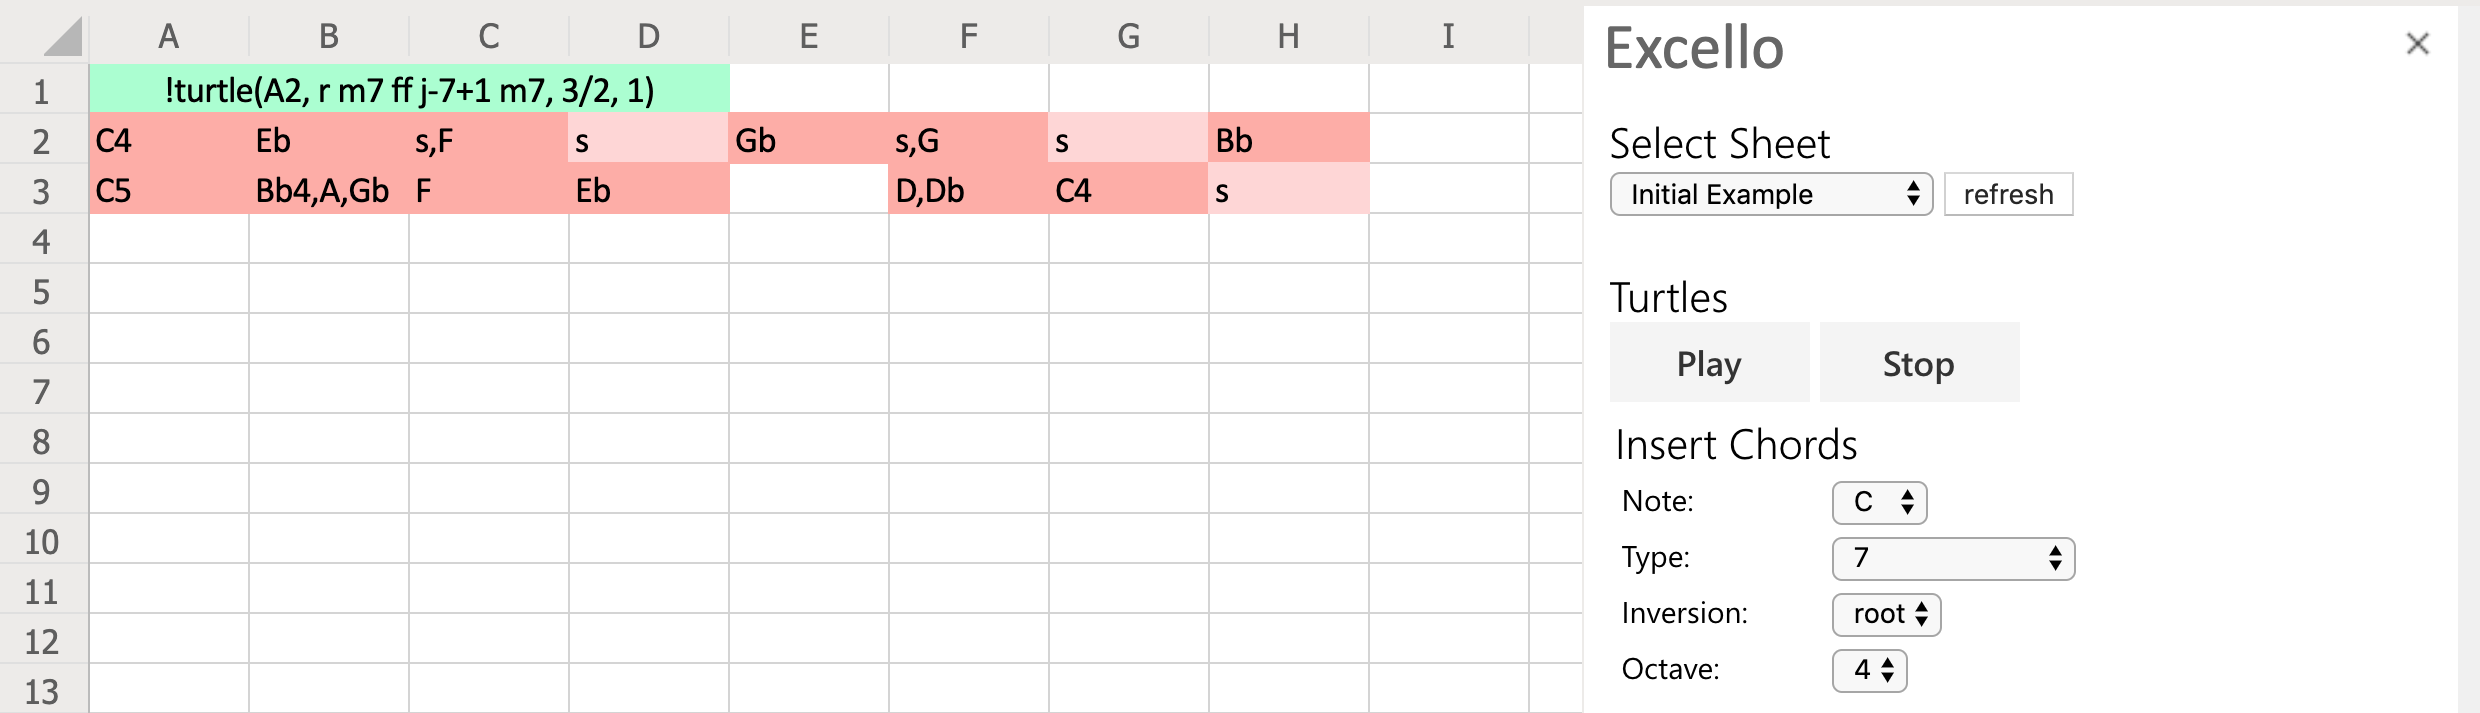
\includegraphics[width=150mm]{figs/initialPrototype.png}}
\caption{A two line motif defined in the initial Excello prototype}
\label{implementation:initialPrototype}
\end{figure}
\begin{figure}[tbh]
\centerline{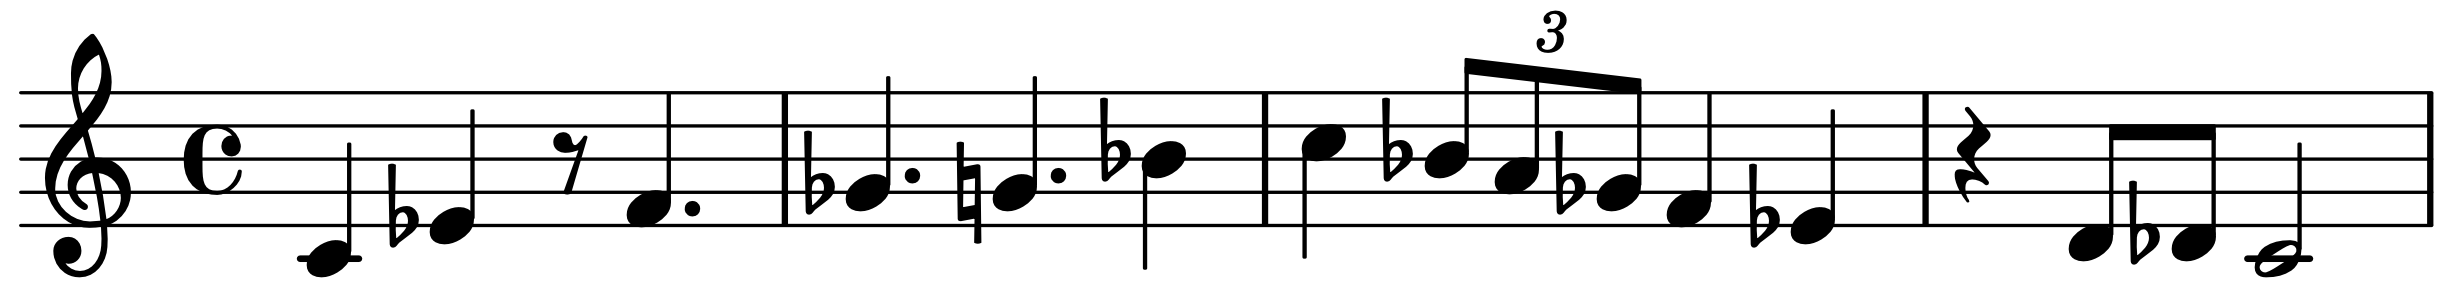
\includegraphics[width=150mm]{figs/initialScore.png}}
\caption{The notes played by the turtle in Figure \ref{implementation:initialPrototype}}
\label{implementation:initialScore}
\end{figure}

\vspace{-10pt}
\paragraph{} Notes and turtles can be defined in any cell. Turtles' interpretation of cells is shown in Table \ref{tab:cells}. When the Excello add-in is opened, a window opens on the right side of Excel as shown in Figure \ref{implementation:initialPrototype}. The melodic line produced is shown in figure \ref{implementation:initialScore}. Play and stop buttons launch all the turtles defined in the spreadsheet and initiate playback with a realistic piano sound.

\begin{table}[htb]
\centering
% \caption{Grammar Rules for the turtle movement instructions. $z \in \Z$}
\vspace{1pt}
\begin{tabular}{|l|l|} \hline
\textbf{Interpretation}&\textbf{Format}\\ \hline
Note& Name (A-G), optional accidental and octave number e.g.~\texttt{F$\sharp$4}\\ \hline
Sustain& \texttt{s}\\ \hline
Multiple notes& Notes, rests or sustains separated by a comma. Rests \\
subdivided in time& must be a space or an empty string e.g.~\texttt{E4,,C4,s}\\ \hline
Rest& Any cell not interpreted as a note, sustain or multi-note. \\ \hline
\end{tabular}
\caption{Interpretation of cells.\label{tab:cells}}
\end{table}

\subsection{Turtles}

\paragraph{} The following formula is enetered into a cell in the grid to define a turtle:\\
\texttt{!turtle(<Starting Cell>, <Movement>, <Speed>, <Number of Loops>)}

\vspace{-5pt}
\subsubsection{Activation}

\paragraph{} The prefix ``\texttt{!}" indicates the turtle will be activated when the play button is pressed. Just as digital audio workstations allow track muting and soloing, this can be used to modify which turtles play, without losing their definitions.

\vspace{-5pt}
\subsubsection{Starting Cell}

\paragraph{} The turtle's starting cell (\texttt{A2} in Figure \ref{implementation:initialPrototype}), which is also played, is a cell reference. As with Excel formulae, this is a concatenation of letters for the column and numbers for the row.

\paragraph{} As each turtle only plays one note at a time, multiple turtles must be defined to play polyphonic music such as chords. It was believed that users would define turtles following identical paths but in adjacent rows or columns. Multiple turtles following identical paths but starting from adjacent cells are defined using the existing Excel range notation for the starting cells. ``\texttt{A2:A5}" would define four turtles in the cells A2,A3,A4,A5. This prevents writing multiple turtle definitions differing in only the start cell row.

\vspace{-5pt}
\subsubsection{Movement}

\paragraph{} Turtles start facing north. The language for programming turtle movement is discussed in the Preparation chapter. The instructions are \texttt{r m7 ff j-7+1 m7} in Figure \ref{implementation:initialPrototype}. Using brackets to repeat movements had not been implemented by the start of the participatory design process.

\vspace{-5pt}
\subsubsection{Speed}

\paragraph{} An optional third argument is the speed of the turtle relative to 160 cells per minute. The default, 1, corresponds to 160 cells per minute. ``\texttt{3/2}", as in Figure \ref{implementation:initialPrototype}, would move the turtle at 240 cells per minute. Relative speed was used so it would be easier to tell the speed relation between turtles. This particularly suits phase music. Arbitrary maths can be provided, allowing turtles' speeds to be irrational multiples of each other.

\vspace{-5pt}
\subsubsection{Number of Loops}

\paragraph{} An optional fourth argument defines the number of repetitions of the turtle's entire path (\texttt{1} in Figure \ref{implementation:initialPrototype}). By default, the turtle loops infinitely. Repeating parts (e.g.~the cello in Pachelbel's Canon in D) therefore only need defining once.

\subsection{Highlighting}

\paragraph{} To assist recognising notes and turtles, when the play button is pressed, cells are highlighted. Activated or deactivated turtle definitions are highlighted green. Cells containing definitions of notes, or multiple notes, are highlighted red. Sustain cells are highlighted a lighter red, showing correspondence to notes whilst maintaining differentiation.

\subsection{Chord Input}

\paragraph{} To use the musical abstractions of chords whilst keeping the paradigm that a turtle is responsible for up to one note at any time, a tool to add chords is included. The note, type, inversion\footnote{Which note of the chord comes first, the other notes ascend from this. This is much like list rotations.} and starting octave of the chord are input into four drop-downs. The insert button enters the notes of the chord into the grid. If a single cell or a range taller than it is wide is highlighted in the spreadsheet, the notes are inserted vertically starting at the top-left of the range. Otherwise, the notes will be inserted horizontally. Whether the turtles are moving horizontally or vertically both chords and arpeggios\footnote{Where the notes of a chord are played individually in rising or descending order.} can be easily defined. Thus, helpful musical abstractions are still available whilst keeping the cleanness of the turtle system.

\section{Formative Evaluation}

\paragraph{} To guide development to best suit users, participants were involved in formative evaluation. Twenty-one University of Cambridge students, across a range of subjects, took part in the participatory design process. Initially, one-on-one tutorials on the initial prototype were given, followed by a short exercise. After these, users were interviewed on how they found Excello, drawing particular attention to actions that they found particularly unintuitive or requiring notable mental effort. Comparisons were made to musical interfaces with which participants were already familiar. The ethical and data handling procedures are discussed in the evaluation chapter.

\paragraph{} To realistically simulate how Excello would be used, participants carried out an exercise of their choice. Often this was transcribing a piece from memory or from traditional notation into the Excello notation. Two exercises were provided if participants had no immediate inspiration; transcribing a piece from western notation or changing existing Excello notation.

\paragraph{} These sessions were carried out in January 2019. Participants were asked to continue using Excello until the summative evaluation sessions in March. Additional feedback was collected as participants used Excello in their own time. This also ensured the summative evaluation was done with users that had sufficient experience of the interface.
% Participants were encouraged to get in contact with any additional issues or suggestions they had during this time.

\subsection{Issues and Suggestions}

\paragraph{} The issues and suggestions from the participatory design process are summarised below.

\subsubsection{Turtle Notation}

\paragraph{} Dynamics in the turtle instructions (e.g. \texttt{ppp m p m mf m ff m}) made establishing the turtle's path harder, as not all commands related to movement (``\texttt{m4}"). As the dynamics weren't next to the notes to which they corresponded, knowing the volume of a note or where to place the dynamics within the turtle to apply to notes in the spreadsheet was challenging. The initial prototype had no way to assign a dynamic to notes in the first cell. The starting cell could be empty, but this was inconvenient for looping parts, as this empty cell would be included in the loop. Users not familiar with western notation dynamics found them unintuitive. Furthermore, these discrete markings do not enable a continuous volume scale.

\paragraph{} When transcribing a piece, dividing its tempo by 160 for the relative speed caused unnecessary work. Users also forgot whether relative speed referred to the time spent in each cell or how quickly the turtle moved. Following the tutorial, users often had to check the position and meaning of turtle arguments.

\paragraph{} As the number of dynamics and movement commands grew, instructions became long and establishing turtle behaviour became cognitively challenging. Some users confused the ``\texttt{s}" within the turtle instructions to mean sustain (as it does in cells) and not south.

\subsubsection{Feedback}

\paragraph{} It was often unknown if pressing play actually registered, especially if the workbook saving delayed Excello's access to the spreadsheet. If a turtle had accidentally been left activated (with ``\texttt{!}"), the entire grid required searching to locate it. Users requested a summary of active turtle locations in addition to the highlighting.

\subsubsection{MIDI conversions}

\paragraph{} Users of production software said importing and exporting MIDI files would be helpful. If working with an existing MIDI file, converting that into the Excello notation would be convenient. Exportation would let Excello be used to create chord sequences, bass lines and the piece structure, before adding additional effects and recording in digital audio work stations.

\subsubsection{Sources of effort when writing}

\paragraph{} After inputting notes into the grid, the number of cells the turtle had to move required counting. As these were often in a straight line, the Excel status bar allowed users to select cells and immediately see how many there were. However, this was still not efficient, and was particularly inconvenient when users were writing notes and periodically testing what they had written so far. Some users instructed turtles to move forward significantly more steps than required to prevent counting. This is not feasible for looping parts. It was suggested that turtles could determine independently how far they should move.

\paragraph{} Instructions with repeated movements such as moving to the end of a line and jumping down to the beginning of a line below, required a lot of repetition.

\paragraph{} Many of the notes in melodic lines are frequently in the same octave. As such, repeatedly writing out the octave number was tiresome. One user made a comparison to LilyPond~\cite{sandberg:lily} where if the note length is not defined, the previous length would be used.

\paragraph{} Some users find it more intuitive to consider a melodic line by the intervals between notes rather than by the note names. A modulated\footnote{Where the pitch of every note in the sequence has moved by the same amount.} melody line required it to be written out again and could not be derived quicker any from the original version.

\subsubsection{Chords}

\paragraph{} Most users used a small subset of the available chord types, but had to find these within a large list. Separation of the more common chords was requested. Initially, notes inserted vertically had the lowest note at the top with pitch increasing down the column. Because higher pitch notes appear higher up the staff, it was suggested that inverting the order would be more intuitive. Initially, it was unclear what the different drop-downs corresponded to, with some users selecting the 7 from the octave number to try and insert a Maj7\footnote{A type of chord where the seventh note in the scale is added.} chord.

\subsubsection{Activation of Turtles}

\paragraph{} When toggling turtles' activations, entering the edit mode for each cell to add or remove the exclamation mark was very tedious.

\section{Second Prototype}

\paragraph{} Following the formative evaluation sessions and feedback, additions and modifications were made to solve the problems and opportunities that arose.

\subsection{Dynamics}

\paragraph{} To help extract a turtle's path and establish notes' volumes, dynamics are instead now inserted in the cells after the note, separated by a space as in Manhattan~\cite{nash:manhattan}. As before, this will apply to all following notes, until the volume is redefined. A single turtle definition with multiple start cells can now play parts of different volume. However, notes in the grid can be limited to only playing at their given volume. To play the same notes at a different volume, a new path must be made. Overall, the new system was believed to be preferable.

\paragraph{} To use a continuous volume scale, in addition to existing dynamic symbols, a number between 0 and 1 can instead be provided where 0 is silent and 1 is equivalent to \texttt{fff}.

\subsection{Nested Instructions}

\paragraph{} Nested instructions with repeats reduce turtle instructions and more easily incorporate repeated sections or movements. Multiple commands placed within parentheses followed by a number are repeated that number of times. Whilst the fourth argument of the turtle repeats the turtle's entire musical output, repetitions within the movement instructions allow paths to be defined more concisely.

\subsection{Absolute Tempo}

\paragraph{} The turtle's speed is now defined by cells per minute, rather than the relative value used initially. However, values less than 10 are interpreted in the original relative way for backwards compatibility with participants' existing work. To maintain consistency in a production version, this will be removed so speed must be defined absolutely. As speed and dynamics are different orders of magnitude, confusion between them is reduced.

\subsection{Custom Excel Functions}

\paragraph{} Two custom Excel functions have been implemented to aid composition. One to define turtles and a second to transpose notes. This allows Excello to take advantage of the functionality of the existing Excel ecosystem; drag-fill, autocomplete, cell referencing, etc.

\vspace{-20pt}
\texttt{\subsubsection{EXCELLO.TURTLE}}

\paragraph{} When writing a formula, a prompt informs users of the position of arguments, and whether they are optional. This outputs the turtle definition as text. All turtles could reference a single cell for their speeds. Relative tempi could then be implemented by the speed argument of each turtle being a multiple of this global speed as shown in Figure \ref{implementation:turtleFunction}.

\begin{figure}[tbh]
\centerline{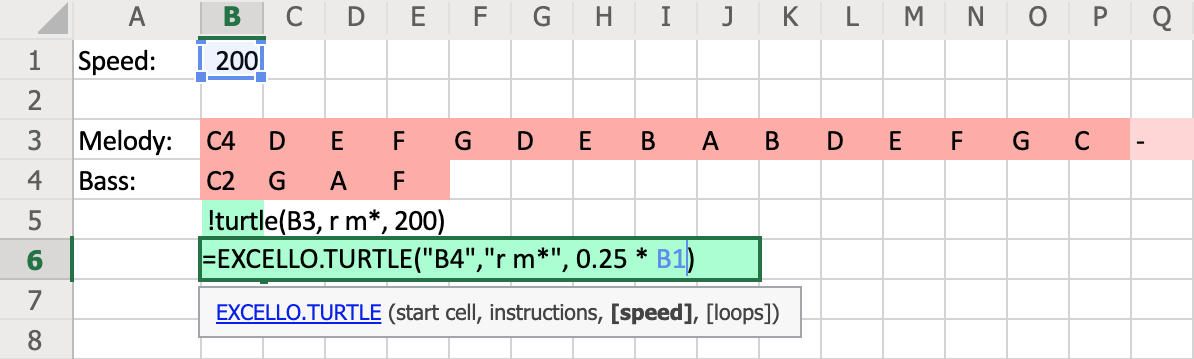
\includegraphics[width=150mm]{figs/turtleFunction.png}}
\caption{Defining a turtle using the \texttt{EXCELLO.TURTLE} function.}
\label{implementation:turtleFunction}
\end{figure}

\vspace{-30pt}
\texttt{\subsubsection{EXCELLO.MODULATE}}

\paragraph{} A modulating function lets melodic lines be defined by the intervals between notes and provides easy modulation of existing sections of a piece. The function takes a cell and an interval and outputs the cell with any notes transposed by the interval, maintaining any dynamics. A section can be modulated by calling this function on the first note with a provided interval and then using drag-fill. By using the previous note and one of a series of intervals as the arguments, a melodic line can quickly be produced from a starting note and a series of intervals as shown in Figure \ref{implementation:modulateFunction}.

\begin{figure}[tbh]
\centerline{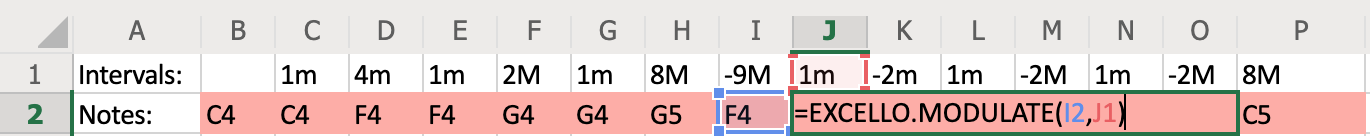
\includegraphics[width=150mm]{figs/modulateFunction.png}}
\caption{Transposing notes using the \texttt{EXCELLO.MODULATE} function.}
\label{implementation:modulateFunction}
\end{figure}

%  \ref{examples}

\subsection{Sustain}

\paragraph{} To prevent confusion between the south instruction and sustains. The symbol ``\texttt{-}" sustains a note. This was chosen because it is light and also has some similarity to a tie.\footnote{A line used in musical notation to increase the length of a note by joining it to another note.} Again, to maintain backwards compatibility, ``\texttt{s}" in a cell is still interpreted as a sustain.

\subsection{Active Turtles}

\paragraph{} To show that active turtle definitions have been recognised, a list of locations of the active turtles is given below the play button. This also helps find spurious turtles not intended to be activated.

\subsection{Automatic Movement}

\paragraph{} To prevent counting the cells in a line, \texttt{m*} instructs a turtle to move as far as there are notes or sustains defined in the direction it is facing. After adding more notes, the turtle instructions do not need editing before pressing play. A part may be meant to finish with a number of rests. As rests are notated with blank cells, a method to extend the path to include these rests was required. A cell can be explicitly defined as a rest with ``\texttt{.}". This is required if multiple turtles are playing a repeating section where one turtle's final cell as a note, sustain or multi-note cell. Without an explicit rest, the turtle would repeat too soon and the parts would consequently be out of phase.

\subsection{Inferred Octave}

\paragraph{} Octave numbers are inferred if omitted. Two methods were considered. Firstly, as most intervals within melodic lines are small, the nearest note could be played.
% This means that a scale would only need the octave defining in the first note.
Whilst this may require the fewest explicit statements of octave numbers, it would be hard to immediately identify the octave of any given note. The last defined octave in the path would need finding and then all subsequent notes walked through keeping track of the octave. The second consideration was to always use the last defined octave. Whilst this may require many octave definitions around the boundary between octaves, it is easier to find the octave of a note by backtracking. The second option was therefore implemented.

\subsection{Chords}

\paragraph{} To aid entering common chords, common types are repeated in a section at the top of the type drop-down. The chord drop-downs layout has been improved with labels to make it clearer what the values refer to. If the notes were entered vertically, the order was reversed, increasing correspondence with traditional staff notation.

\subsection{Activation of turtles}

\paragraph{} A ``Toggle Activation" button was added to the add-in window. When a cell or range is highlighted in the spreadsheet, the activation of any turtle definitions in this range will be toggled when the button is pressed.  This significantly decreases the time to toggle activations, as only two clicks are required, rather than entering the cell edit mode to add or remove an exclamation mark.

\section{Final Prototype Implementation}

\paragraph{} This section discusses the underlying implementation of the final prototype, following the participatory design. Excello consists of three main parts: the turtle system for playing the grid contents, the chord input tool, and the custom Excel functions.

\paragraph{} When the play button is pressed, turtle definitions in the grid are identified. For each, the starting cell and movement instructions are used to establish the contents of the cells it passes through. This is converted to a series of note definitions - pitch, start time, duration, volume. The speed and loop parameters are used to create the structure interpreted by the Tone.js library to schedule and initiate playback. An overview of the data flow and subtasks required to create the musical playback is shown in Figure \ref{fig:overview}.

\begin{figure}[htb]
\begin{center}
  
  \tikzset{every picture/.style={line width=0.75pt}} %set default line width to 0.75pt

  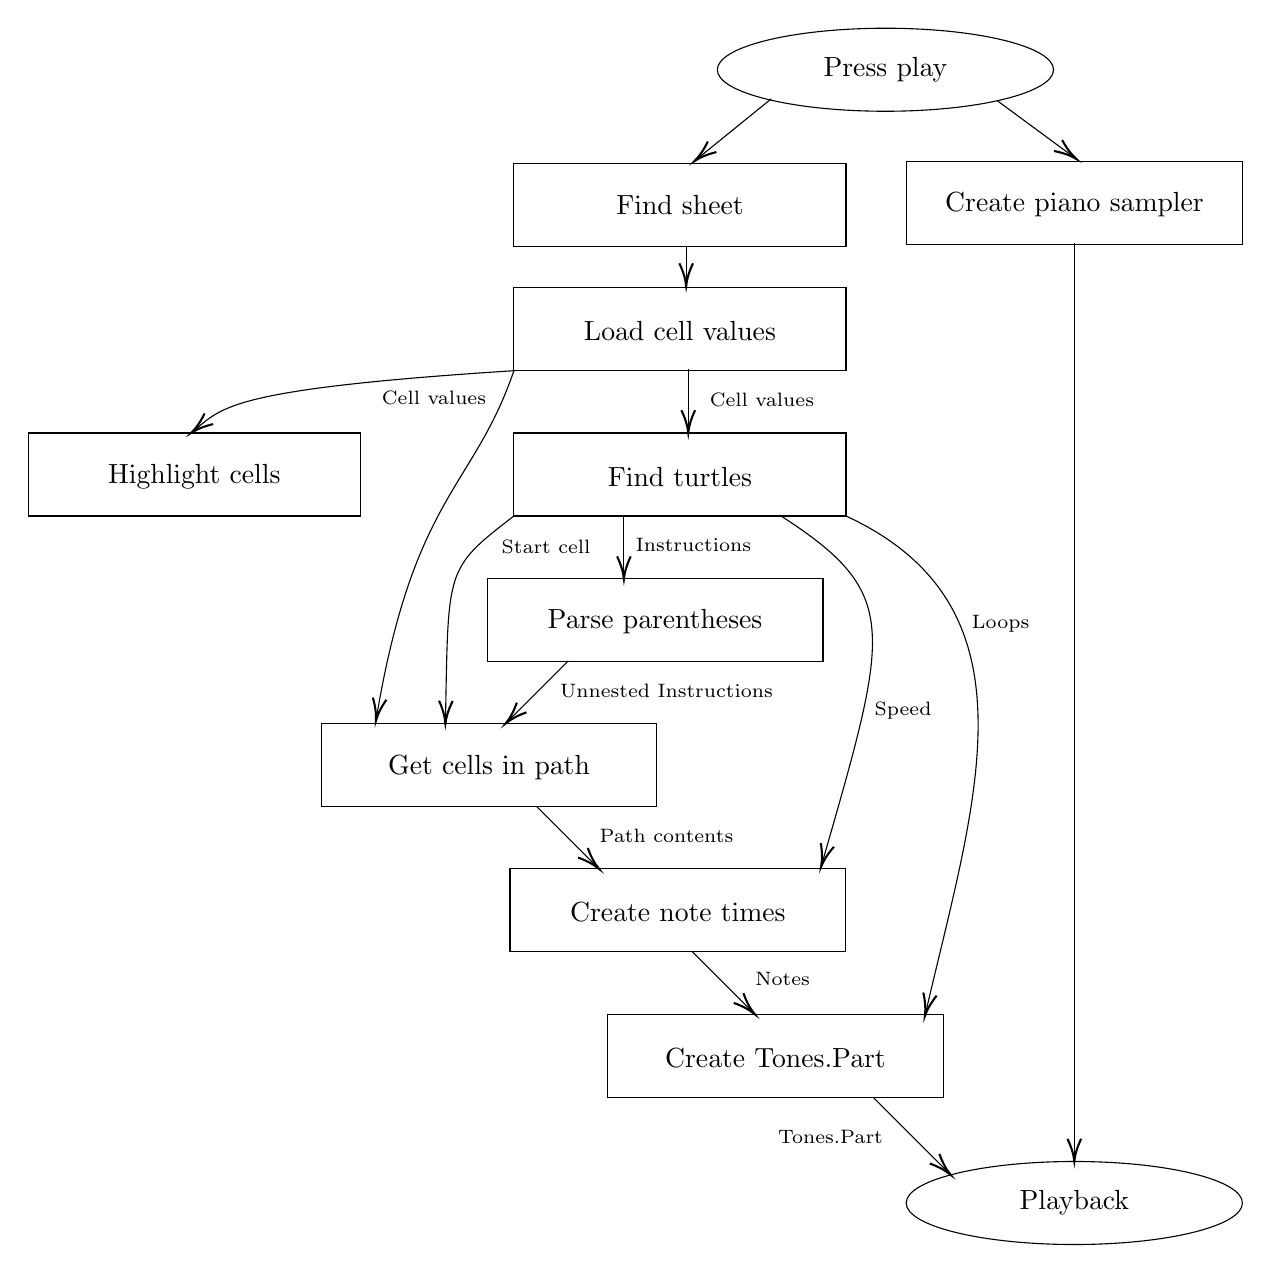
\begin{tikzpicture}[x=0.75pt,y=0.75pt,yscale=-1,xscale=1]
  %uncomment if require: \path (0,604); %set diagram left start at 0, and has height of 604

  %Shape: Rectangle [id:dp3390223975782729]
  \draw   (244.5,71) -- (404.5,71) -- (404.5,111) -- (244.5,111) -- cycle ;

  %Shape: Rectangle [id:dp7168559924493858]
  \draw   (244.5,131) -- (404.5,131) -- (404.5,171) -- (244.5,171) -- cycle ;

  %Shape: Rectangle [id:dp8835932361497658]
  \draw   (433.7,70) -- (595.5,70) -- (595.5,110) -- (433.7,110) -- cycle ;

  %Shape: Rectangle [id:dp9464422191216635]
  \draw   (244.5,201) -- (404.5,201) -- (404.5,241) -- (244.5,241) -- cycle ;

  %Shape: Rectangle [id:dp6384624480751633]
  \draw   (231.6,271) -- (393.4,271) -- (393.4,311) -- (231.6,311) -- cycle ;

  %Shape: Rectangle [id:dp2927464084046889]
  \draw   (151.6,341) -- (313.4,341) -- (313.4,381) -- (151.6,381) -- cycle ;

  %Shape: Rectangle [id:dp9052659554068596]
  \draw   (242.6,411) -- (404.4,411) -- (404.4,451) -- (242.6,451) -- cycle ;

  %Shape: Rectangle [id:dp5637329489183025]
  \draw   (289.6,481) -- (451.4,481) -- (451.4,521) -- (289.6,521) -- cycle ;

  %Curve Lines [id:da3917180624639185]
  \draw    (244.5,241) .. controls (211.17,266.67) and (212.98,265.81) .. (211.52,339.88) ;
  \draw [shift={(211.5,341)}, rotate = 271.14] [color={rgb, 255:red, 0; green, 0; blue, 0 }  ][line width=0.75]    (10.93,-3.29) .. controls (6.95,-1.4) and (3.31,-0.3) .. (0,0) .. controls (3.31,0.3) and (6.95,1.4) .. (10.93,3.29)   ;

  %Straight Lines [id:da6961662223442007]
  \draw    (297.5,241) -- (297.5,269.4) ;
  \draw [shift={(297.5,271.4)}, rotate = 270] [color={rgb, 255:red, 0; green, 0; blue, 0 }  ][line width=0.75]    (10.93,-3.29) .. controls (6.95,-1.4) and (3.31,-0.3) .. (0,0) .. controls (3.31,0.3) and (6.95,1.4) .. (10.93,3.29)   ;

  %Curve Lines [id:da9168950950169605]
  \draw    (372.6,240.6) .. controls (431.31,278.41) and (425.56,294.84) .. (392.99,408.28) ;
  \draw [shift={(392.5,410)}, rotate = 286.01] [color={rgb, 255:red, 0; green, 0; blue, 0 }  ][line width=0.75]    (10.93,-3.29) .. controls (6.95,-1.4) and (3.31,-0.3) .. (0,0) .. controls (3.31,0.3) and (6.95,1.4) .. (10.93,3.29)   ;

  %Curve Lines [id:da7972588626438504]
  \draw    (404.5,241) .. controls (499.03,284.78) and (466.83,377.07) .. (442.86,480.44) ;
  \draw [shift={(442.5,482)}, rotate = 282.99] [color={rgb, 255:red, 0; green, 0; blue, 0 }  ][line width=0.75]    (10.93,-3.29) .. controls (6.95,-1.4) and (3.31,-0.3) .. (0,0) .. controls (3.31,0.3) and (6.95,1.4) .. (10.93,3.29)   ;

  %Straight Lines [id:da6822022155717844]
  \draw    (270.7,310.8) -- (241.91,339.59) ;
  \draw [shift={(240.5,341)}, rotate = 315] [color={rgb, 255:red, 0; green, 0; blue, 0 }  ][line width=0.75]    (10.93,-3.29) .. controls (6.95,-1.4) and (3.31,-0.3) .. (0,0) .. controls (3.31,0.3) and (6.95,1.4) .. (10.93,3.29)   ;

  %Straight Lines [id:da4884596231580207]
  \draw    (255.5,381) -- (284.09,409.59) ;
  \draw [shift={(285.5,411)}, rotate = 225] [color={rgb, 255:red, 0; green, 0; blue, 0 }  ][line width=0.75]    (10.93,-3.29) .. controls (6.95,-1.4) and (3.31,-0.3) .. (0,0) .. controls (3.31,0.3) and (6.95,1.4) .. (10.93,3.29)   ;

  %Straight Lines [id:da9233366942734922]
  \draw    (330.5,451) -- (359.09,479.59) ;
  \draw [shift={(360.5,481)}, rotate = 225] [color={rgb, 255:red, 0; green, 0; blue, 0 }  ][line width=0.75]    (10.93,-3.29) .. controls (6.95,-1.4) and (3.31,-0.3) .. (0,0) .. controls (3.31,0.3) and (6.95,1.4) .. (10.93,3.29)   ;

  %Straight Lines [id:da3670498457872964]
  \draw    (417.5,521) -- (453.49,556.99) ;
  \draw [shift={(454.9,558.4)}, rotate = 225] [color={rgb, 255:red, 0; green, 0; blue, 0 }  ][line width=0.75]    (10.93,-3.29) .. controls (6.95,-1.4) and (3.31,-0.3) .. (0,0) .. controls (3.31,0.3) and (6.95,1.4) .. (10.93,3.29)   ;

  %Straight Lines [id:da28794703530347365]
  \draw    (327.5,111) -- (327.5,128.2) ;
  \draw [shift={(327.5,130.2)}, rotate = 270] [color={rgb, 255:red, 0; green, 0; blue, 0 }  ][line width=0.75]    (10.93,-3.29) .. controls (6.95,-1.4) and (3.31,-0.3) .. (0,0) .. controls (3.31,0.3) and (6.95,1.4) .. (10.93,3.29)   ;

  %Straight Lines [id:da33376731250782754]
  \draw    (328.5,170) -- (328.5,199) ;
  \draw [shift={(328.5,201)}, rotate = 270] [color={rgb, 255:red, 0; green, 0; blue, 0 }  ][line width=0.75]    (10.93,-3.29) .. controls (6.95,-1.4) and (3.31,-0.3) .. (0,0) .. controls (3.31,0.3) and (6.95,1.4) .. (10.93,3.29)   ;

  %Curve Lines [id:da2676626927985757]
  \draw    (244.5,171) .. controls (225.1,227.72) and (196.29,230.77) .. (178.27,338.17) ;
  \draw [shift={(178,339.8)}, rotate = 279.38] [color={rgb, 255:red, 0; green, 0; blue, 0 }  ][line width=0.75]    (10.93,-3.29) .. controls (6.95,-1.4) and (3.31,-0.3) .. (0,0) .. controls (3.31,0.3) and (6.95,1.4) .. (10.93,3.29)   ;

  %Straight Lines [id:da024649031996502035]
  \draw    (514.5,109.6) -- (514.5,550) ;
  \draw [shift={(514.5,552)}, rotate = 270] [color={rgb, 255:red, 0; green, 0; blue, 0 }  ][line width=0.75]    (10.93,-3.29) .. controls (6.95,-1.4) and (3.31,-0.3) .. (0,0) .. controls (3.31,0.3) and (6.95,1.4) .. (10.93,3.29)   ;

  %Shape: Ellipse [id:dp13505581605963868]
  \draw   (433.5,572) .. controls (433.5,560.95) and (469.76,552) .. (514.5,552) .. controls (559.24,552) and (595.5,560.95) .. (595.5,572) .. controls (595.5,583.05) and (559.24,592) .. (514.5,592) .. controls (469.76,592) and (433.5,583.05) .. (433.5,572) -- cycle ;

  %Shape: Ellipse [id:dp006287630832967794]
  \draw   (342.5,26) .. controls (342.5,14.95) and (378.76,6) .. (423.5,6) .. controls (468.24,6) and (504.5,14.95) .. (504.5,26) .. controls (504.5,37.05) and (468.24,46) .. (423.5,46) .. controls (378.76,46) and (342.5,37.05) .. (342.5,26) -- cycle ;

  %Straight Lines [id:da09048722077694915]
  \draw    (368.5,40) -- (333.05,68.74) ;
  \draw [shift={(331.5,70)}, rotate = 320.96000000000004] [color={rgb, 255:red, 0; green, 0; blue, 0 }  ][line width=0.75]    (10.93,-3.29) .. controls (6.95,-1.4) and (3.31,-0.3) .. (0,0) .. controls (3.31,0.3) and (6.95,1.4) .. (10.93,3.29)   ;

  %Straight Lines [id:da9578993167654264]
  \draw    (477.5,41) -- (513.89,67.81) ;
  \draw [shift={(515.5,69)}, rotate = 216.38] [color={rgb, 255:red, 0; green, 0; blue, 0 }  ][line width=0.75]    (10.93,-3.29) .. controls (6.95,-1.4) and (3.31,-0.3) .. (0,0) .. controls (3.31,0.3) and (6.95,1.4) .. (10.93,3.29)   ;

  %Shape: Rectangle [id:dp25073410390478523]
  \draw   (10.5,201) -- (170.5,201) -- (170.5,241) -- (10.5,241) -- cycle ;

  %Curve Lines [id:da2454539812308738]
  \draw    (244.5,171) .. controls (108.92,179.69) and (104.17,188.37) .. (90.53,199.75) ;
  \draw [shift={(89,201)}, rotate = 321.34000000000003] [color={rgb, 255:red, 0; green, 0; blue, 0 }  ][line width=0.75]    (10.93,-3.29) .. controls (6.95,-1.4) and (3.31,-0.3) .. (0,0) .. controls (3.31,0.3) and (6.95,1.4) .. (10.93,3.29)   ;


  % Text Node
  \draw (324.5,91) node  [align=left] {Find sheet};
  % Text Node
  \draw (324.5,152) node  [align=left] {Load cell values};
  % Text Node
  \draw (514.6,91) node  [align=left] {Create piano sampler};
  % Text Node
  \draw (324.5,222) node  [align=left] {Find turtles};
  % Text Node
  \draw (312.5,292) node  [align=left] {Parse parentheses};
  % Text Node
  \draw (232.5,362) node  [align=left] {Get cells in path};
  % Text Node
  \draw (323.5,432) node  [align=left] {Create note times};
  % Text Node
  \draw (370.5,502) node  [align=left] {Create Tones.Part};
  % Text Node
  \draw (514.5,572) node [] [align=left] {\textcolor[rgb]{0,0,0}{Playback}};
  % Text Node
  \draw (260,256) node  [align=left] {{\scriptsize Start cell}};
  % Text Node
  \draw (331,255) node  [align=left] {{\scriptsize Instructions}};
  % Text Node
  \draw (432,335) node  [align=left] {{\scriptsize Speed}};
  % Text Node
  \draw (479,293) node  [align=left] {{\scriptsize Loops}};
  % Text Node
  \draw (318,325) node  [align=left] {{\scriptsize Unnested Instructions}};
  % Text Node
  \draw (318,395) node  [align=left] {{\scriptsize Path contents}};
  % Text Node
  \draw (374,464) node  [align=left] {{\scriptsize Notes}};
  % Text Node
  \draw (397,540) node  [align=left] {{\scriptsize Tones.Part}};
  % Text Node
  \draw (206,184) node  [align=left] {{\scriptsize Cell values}};
  % Text Node
  \draw (423.5,26) node [] [align=left] {Press play};
  % Text Node
  \draw (364,185) node  [align=left] {{\scriptsize Cell values}};
  % Text Node
  \draw (90.5,222) node  [align=left] {Highlight cells};


  \end{tikzpicture}

\end{center}
\caption{An overview of the playback algorithm and dataflow of Excello\label{fig:overview}}
\end{figure}

\paragraph{} The \texttt{Sampler} is an extension of the \texttt{Tone.Instrument} class. This interpolates between pitched samples to create arbitrary notes. A sampler is loaded using the Salamander grand piano samples~\footnote{https://freepats.zenvoid.org/Piano/acoustic-grand-piano.html} which includes four pitches (out of a possible 12) per octave. This accurately interpolates notes whilst reducing loading times and storage requirements.

\subsection{Identifying Cells}

\paragraph{} A drop-down is populated with names loaded using the Office API. Having pressed play, the cell values from the selected sheet are loaded and then analysed for highlighting and calculating the musical output. Cells containing at least one note definition are highlighted red. A note must contain a note name, optional accidental, optional octave number, and optional volume instruction following a space. This is a dynamic marking or number between 0 and 1. Notes are identified using the following regular expression:

\begin{verbatim}
^[A-G](#|b|)?[1-9]?( (0(\.\[0-9]+)?|1(\.0)?|ppp|pp|p|mp|mf|f|ff|fff))?$
\end{verbatim}

\paragraph{} Cells containing multiple definitions (e.g. ``\texttt{C4 ff,-, ,D}", ``\texttt{,,G,F$\sharp$}") are split using commas. The resulting strings are trimmed of starting and ending whitespace and then must either be a note, sustain (``\texttt{-}" or ``\texttt{s}"), explicit rest (``\texttt{.}") or empty string (created from trimming a rest). Cells matching ``\texttt{-}",``\texttt{.}" or ``\texttt{s}" are highlighted a lighter red. Turtle definitions (e.g. ``\texttt{!turtle(B2:B4, r m*, 200, 1)}") are identified using:
\begin{verbatim}
^(!turtle\().*(\))$
\end{verbatim}
and these cells are highlighted green. The addresses of cells containing a turtle definition are added to the live turtle section of the add-in window.

\subsection{Parsing Movement Instructions}

\paragraph{} Movement instructions are converted to a single unnested list of commands (e.g.~``\texttt{(r m2)2}" becomes ``\texttt{[r, m2, r, m2]}") so the turtle's path can be established. The \texttt{parse} method of the Parenthesis\footnote{https://www.npmjs.com/package/parenthesis} library seemed suitable for aiding this string manipulation. This parses strings containing brackets into a nested array. For example, \texttt{parse(\textcolor[rgb]{0,0.7,0}{\upquote{a(b[c\{d\}])}})} gives \texttt{[\textcolor[rgb]{0,0.7,0}{\upquote{a(}}, [\textcolor[rgb]{0,0.7,0}{\upquote{b[}}, [\textcolor[rgb]{0,0.7,0}{\upquote{c\{}}, [\textcolor[rgb]{0,0.7,0}{\upquote{d}}], \textcolor[rgb]{0,0.7,0}{\upquote{\}}}], \textcolor[rgb]{0,0.7,0}{\upquote{]}}], \textcolor[rgb]{0,0.7,0}{\upquote{)}}]}.

\paragraph{} This suggests the string ``\texttt{(r m2)2}" would become \texttt{[\upquote{(}, [\upquote{r m2}], \upquote{)2}]}. By removing the brackets from these strings, a simple recursive method could be built to output \texttt{\upquote{r m2 r m2}} from \texttt{[[\upquote{r m2}], \upquote{2}]}. However, upon testing this, the library outputted an undefined array. From investigating the source code, I established that strings with a number following a closing parenthesis all produced this error. Substituting characters for the numbers or placing a symbol before all numbers and then later removing these would allow the library to be used. Instead, using the Parenthesis method as inspiration, I implemented my own parsing function tailored to Excello.

\paragraph{} This has two main steps. First, the deepest bracketed expression is stored in an array with the brackets removed. This expression is replaced in the original string with the string \upquote{\texttt{\_\_\_}$x$\texttt{\_\_\_}} where $x$ is the expression's index in the array. This is repeated until the string contains no brackets. Then a recursive function uses the values of $x$ to reconstruct the string in the nested array format. This method is outlined in Algorithm \ref{alg:parenthesis}. The Typescript implementation is in Appendix \ref{appendix:parseBrackets}.

\begin{algorithm}[!htp]
\caption{Parsing bracketed expression. \texttt{str.replace(regex,f)} (line 13) performs \texttt{f(s)} on the first substring, \texttt{s}, of \texttt{str} matching the regular expression \texttt{regex}.}
\label{alg:parenthesis}
\begin{algorithmic}[1]
\Procedure{parseBrackets}{$str$}

   \State $idPadding\gets \texttt{\upquote{\_\_\_}}$
   \State $unnestedStr\gets []$
   \State $deepestLevelBracketsRE\gets \texttt{RegExp(\upquote{\textbackslash\textbackslash([\^{}\textbackslash\textbackslash(\textbackslash\textbackslash)]*\textbackslash\textbackslash)})}$
   \State $replacementIDRE\gets \texttt{RegExp(\upquote{\textbackslash\textbackslash} + }idPadding\texttt{ + \upquote{([0-9]+)} + }idPadding\texttt{)}$\\

   \Procedure{replaceDeepestBracket}{$x$}
     \State \texttt{unnestedStr.push(x.substring(1, x.length-1))}
     \State \texttt{\textbf{return} idPadding + (unnestedStr.length - 1) + idPadding}
   \EndProcedure \\

   \While{\texttt{deepestLevelBracketsRE.test(str)}}
     \State \texttt{str = str.replace(deepestLevelBracketsRE,replaceDeepestBracket)}
   \EndWhile

   \State \texttt{unnestedStr[0] = str}\\

   \Procedure{reNest}{$outerStr$}
     \State $renestingStr\gets []$
     \While{There is a match of $replacementIDRE$ in $outerStr$}
       \State $matchIndex\gets$ index of the match in $outerStr$
       \State $matchID\gets$ ID of the match (number between padding)
       \State $matchString\gets$ matched string\\

       \If{$matchIndex >$ 0}
				\State $renestingStr$.push($outestStr$.substring(0, $matchIndex$))
			\EndIf
			\State $renestingStr$.push(reNest($unnestedStr$[$firstMatchID$]))
			\State $outestStr$ = $outestStr$.substring($matchIndex$ + $matchString$.length)
     \EndWhile
     \State $renestingStr$.push($outestStr$)
     \State \textbf{return} $renestingStr$
   \EndProcedure \\

   \State \textbf{return} \textsc{reNest}($unnestedStr$[0])

\EndProcedure
\end{algorithmic}
\end{algorithm}


\paragraph{} Having submitted a bug report on the Parenthesis GitHub, and implemented my own method for parsing turtle movement instructions, I implemented a fix to the Parenthesis library. The library previously performed replacements with the string \upquote{\texttt{\_\_\_}$x$}. $x$ and following numbers would concatenate forming a single number, causing the library to fail. My method of having an identifier before and after $x$ fixed this issue. I also added additional tests to Parenthesis to verify my method and ensure that previous tests all passed before submitting a pull request. I have made an open source contribution, as this has since been merged into the library and published.

\paragraph{} I wrote an additional recursive method to unnest the array into a single stream of commands. An empty string, \texttt{s}, is initialised. For each item in the array, if it is an array, unnest the contents recursively and add the result to s. If not, it will be one or more single movement commands. If the single movement commands start with a number, the result is added to \texttt{s} that number of times. The remaining instructions are added to \texttt{s}. This is outlined in Algorithm \ref{alg:unnest}. The implementation is shown in Appendix \ref{appendix:processParsedBrackets}.

\begin{algorithm}[!htbp]
\caption{Unnesting parsed bracketed expressions.}
\label{alg:unnest}
\begin{algorithmic}[1]
\Procedure{processParsedBrackets}{$arr$}

   \State $s\gets \texttt{\upquote{}}$
   \State $previousArr$

   \For{$v$ in $s$}
    \If{$v$ is an array}
     \State $previousArr \gets$ processParsedBrackets($v$)
    \Else
       \If{previous instruction was an array}
        \State $s \gets s + previousArr$
        \If{next instruction is a number}
          \State $s \gets s + previousArr$, that number of times minus one
        \EndIf
       \EndIf
       \State $s \gets s + $ remaining instruction in $v$
    \EndIf
   \EndFor
   \State \textbf{return} $s$

\EndProcedure
\end{algorithmic}
\end{algorithm}

\subsection{Getting Cells in Turtles' Paths}

\paragraph{} If the turtle's first argument defines a range of starting cells, the cell addresses of this range are calculated. For each starting cell, the unnested instructions and sheet values are used to find the contents of the cells the turtle passes through. This process models the movement of the turtle within the grid, keeping track of its position and the direction in which it is facing. For each instruction, the position and direction are updated as required, and the contents of any new cells entered are added to a list of notes.

\paragraph{} For the ``\texttt{m*}" instruction, the number of steps the turtle takes must be computed. Given the turtle's current position and direction, the one-dimensional array of cells in front of it is taken. The turtle should step to the last cell that defines a note, sustain or explicit rest. The number of steps is the array's length minus the index of the first element in the reversed array satisfying this criterion.

\subsection{Creating Note Times}

\paragraph{} The cells a turtle moves through are used to create a data structure containing the information for playback using the Tone library. For each turtle, the following array is produced: \texttt{[[<Note 1>,...,<Note N>], <number of cells>]} (note sequence array). Each note is as follows: \texttt{[<start time>, [<pitch>, <duration>, <volume>]]}. Volume and octave are added to each note if they were omitted from a cell.

\paragraph{} The Tone Transport is a timeline along which events can be scheduled. This supports many different representations of time. I used Transport Time for all note onsets and durations. This is of the form \texttt{\upquote{BARS:QUARTERS:SIXTEENTHS}} where the three values are numbers and can be non-integer. With \texttt{QUARTERS} representing the number of cells, the calculation of exact times, or arbitrary musical notes can be avoided. This allows the contents of cells to be easily converted to times to be interpreted by the Tones library.

\paragraph{} The note sequence array is initiated by counting the notes that are defined in the cell contents using regular expressions for identifying notes and multi-note cells. The cells are iterated through keeping track of the active note and adding it to the note sequence when it ends. Outside of this loop, variables track how many cells and notes through the process the algorithm is and whether it is currently a rest or note. Variables keep track of the note currently being played - when it started (\texttt{currentStart}), the pitch (\texttt{currentNote}) and the volume (\texttt{currentVolume}). As volume and octave number may be omitted, variables also keep track of these. Table \ref{tab:times} outlines the actions performed when a cell is read. Notes are added to the note sequence in the form \texttt{[currentStart, [currentNote, \upquote{0:} + noteLength + \upquote{:0}, currentVolume]]}.

\begin{table}[ht]
\begin{tabular}{|l|l|l|l|l|}
  \hline
  \textbf{Cell}&\textbf{State}&\multicolumn{3}{c|}{\textbf{Action}} \\
  \hline
  \multirow{5}{*}{Note}&\multirow{3}{*}{Note}&Note, octave and &Previous note added&currentStart = \\
  &&volume established&to note sequence&\upquote{0:}+beatCount+\upquote{:0}\\
  &&from cell contents&&currentNote = value\\
  \cline{2-2}
  \cline{4-4}
  &\multirow{2}{*}{Rest}&and previous values&inRest = false&noteLength = 1\\
  &&&&currentVolume = volume\\
  \hline
  \multirow{2}{*}{Sustain}&Note&\multicolumn{3}{l|}{noteLength++}\\
  \cline{2-5}
  &Rest&\multicolumn{3}{l|}{Nothing (has no semantic value)}\\
  \hline
  \multirow{3}{*}{Rest}&\multirow{2}{*}{Note}&\multicolumn{3}{l|}{Previous note added to note sequence}\\
  &&\multicolumn{3}{l|}{inRest = true}\\
  \cline{2-5}
  &Rest&\multicolumn{3}{l|}{Nothing}\\
  \hline
\end{tabular}
\caption{The actions taken when processing each cell to create note times. The beat count corresponds to the cell number being processed and is incremented each time.\label{tab:times}}
\end{table}
\vspace{-10pt}

\paragraph{} The same method is used for multi-note cells, except the note length and cell count are incremented by the appropriate fraction for each item in the cell. If, after the final cell, the state is a note, it is ended and added to the note sequence.

\paragraph{} The values in the note sequence are sufficient for the piano sampler to play a note using the \texttt{triggerAttackRelease} function. The \texttt{Tone.Part} class allows multiple calls to this method to be defined, started, stopped and looped as a single unit. This is defined with the note sequence and its speed set with the evaluated turtle speed argument. The number of cells, calculated when creating the note times, number of repeats, and the evaluated speed argument are used to control when looping ends.

% \begin{verbatim}
% var turtlePart = new Tone.Part(function(time, note){
%   piano.triggerAttackRelease(note[0], note[1], time, note[2]);
% }, noteTimes).start();
% if (repeats>0){
%   turtlePart = turtlePart.stop("0:" + (repeats*beatsLength/speedFactor) + ":0");
% }
% turtlePart.loop = true;
% turtlePart.loopEnd = "0:" + beatsLength + ":0";
% turtlePart.playbackRate = speedFactor;
% \end{verbatim}

% \begin{lstlisting}[style=js]
%   var turtlePart = new Tone.Part(function(time, note){
%     piano.triggerAttackRelease(note[0], note[1], time, note[2]);
%   }, noteTimes).start();
%   if (repeats>0){
%     turtlePart = turtlePart.stop("0:" + (repeats*beatsLength/speedFactor) + ":0");
%   }
%   turtlePart.loop = true;
%   turtlePart.loopEnd = "0:" + beatsLength + ":0";
%   turtlePart.playbackRate = speedFactor;
% \end{lstlisting}

\subsection{Chord Input}\label{Chord Input}

\paragraph{} The next two subsections (\S\ref{Chord Input} and \S\ref{Custom Excel Functions}) outline the two smaller parts of the Excello; the chord input tool, and the custom Excel functions. When the insert button in the add-in window is pressed, the note, type, inversion and octave of the chord are extracted from their HTML elements. The chord interface within the add-in window is shown in Figure \ref{fig:chordInput}. The tonal library is used to generate the chord notes:

\begin{verbatim}
var chordNotes = Chord.notes(chordNote, chordType).map(x => Note.simplify(x));
\end{verbatim}
\vspace{-10pt}

\begin{figure}[htb]
\centerline{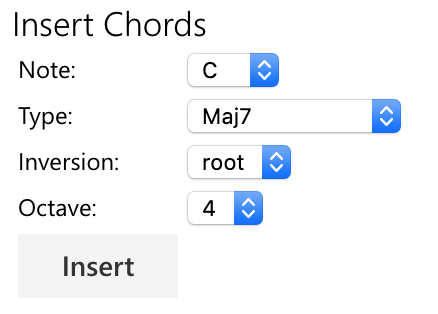
\includegraphics[width=50mm]{figs/insertChord.png}}
\caption{The interface within the add-in window for inserting the notes of chords.}
\label{fig:chordInput}
\end{figure}

\vspace{-20pt}
\paragraph{} The tonal \texttt{simplify} function reduces note definitions to contain at most one accidental, as required by Excello. This provides a list of notes in ascending order, without octaves or taking into account the inversion. To create the correct inversion of the chord, the array of notes is rotated by the inversion number.

\paragraph{} The given octave number is appended to the first note. A dictionary matches note names, accounting for enharmonics,\footnote{Notes that are the same pitch but different names, such as A$\flat$ and G$\sharp$.} to position in the chromatic scale starting at C (the first note of the octave in SPN). For each preceding note, if it appears in an equal or lower position in the scale than its predecessor, the octave number is incremented before appending. Otherwise, it is in the same octave, so the octave number is appended without modification.

\paragraph{} The selected range is acquired with the Office API. The chord notes are entered starting at the top-left corner of this range. If the range's height is greater or equal to its width, the notes are entered vertically going down. Otherwise, they are entered horizontally going right. Using the Office API, the range is set to the 2D array where the chord is entered.

\subsection{Custom Excel Functions}\label{Custom Excel Functions}

\paragraph{} Custom functions are implemented using another add-in. Rather than a separate window like the main Excello add-in, additional functions can be used in cells with the prefix ``\texttt{=EXCELLO.}". The file structure was generated with the Yeoman generator. The name, description, result type, and parameter names and types are stored in a JSON schema. This is used by Excel to provide argument prompts and autofill when writing formulae. Functions are defined in Typescript.

\paragraph{} The turtle function concatenates the arguments into the Excello turtle format. Other cells can be referenced, for example, the speed variable can reference a global tempo variable as in Figure \ref{implementation:turtleFunction}.

\paragraph{} The modulation function separates the note and volume for every note defined in a cell. The note is modulated using the tonal \texttt{Distance.transpose} function and recombined with the volume. The drag fill feature of Excel can be employed by the user to transpose sections or define melodic lines using the interval between notes as in Figure \ref{implementation:modulateFunction}.

\section{MIDI Converter}

\paragraph{} This section explains the Python converter from MIDI to CSV for Excello playback. A MIDI file is divided into up to 16 parallel tracks~\cite{midiSpec}. Each track contains a series of messages defined using predefined status and data bytes. I used the Mido library\footnote{https://mido.readthedocs.io/en/latest/index.html} to read MIDI files and abstract away from the underlying byte representations to view the messages. Note onsets and offsets are two separate events with two separate messages~\cite{midiSpec}. These messages include the note pitch, velocity, channel (not relevant) and time in ticks since the last message~\cite{midoSpec}.

\paragraph{} First, the list of messages is converted to a list of notes defined by onset and offset time, pitch and velocity. For each track, the messages are iterated through, using the time value in every message (including control and meta messages) to update a variable tracking time. For note onset messages, this is added to a dictionary mapping pitch to a list of currently active note start times. Lists are used because a pitch can be active multiple times at once. For note offset messages, or onset messages with zero velocity, the note popped from the active notes at that pitch with end time added is added to the list of all notes defined in the file.

\paragraph{} As each turtle only plays one note at a time, the notes are split into lists so no list contains concurrently played notes. Provided the initial list of notes is non-empty, a new list is created. The first remaining note is moved to the new list. Then iterating over the remaining notes, the next note starting after the previous note ends is moved to this new list. The number of iterations required is the number of turtles, $n$.

\paragraph{} If every tick corresponds to a cell, any combination of note onsets and offsets in a MIDI file can be accurately represented in Excello. To achieve smaller representations, the start and end times are converted to smaller cell numbers within the path of the turtle. For many MIDI files, the duration of a note is different from the time it occupies in notation. For example, a note immediately followed by another note in notation may have an end time significantly less than the start time of the next note in MIDI. A method is required to account for this. For all notes, before creating the different turtle streams, the length of the notes in ticks and differences between consecutive start times are found. The minimum value greater than 1 or modal value for these times are calculated depending on the compression level giving the $lengthStat$ and $di\hspace{-0.1em}f\hspace{-0.2em}f\hspace{-0.1em}erenceStat$.
\vspace{-10pt}

  $$ratio_{int} = \lfloor\max(lengthStat, di\hspace{-0.1em}f\hspace{-0.2em}f\hspace{-0.1em}erenceStat)/\min(lengthStat, di\hspace{-0.1em}f\hspace{-0.2em}f\hspace{-0.1em}erenceStat)\rfloor$$
  % $$ratio_{int} = \lfloor ratio \rfloor$$
  % $$correction = ratio/ratio_{int}$$
For each note, the times are adjusted as follows:
  $$length \gets (start - end) / lengthStat \text{ (rounded to the nearest 0.1)}$$
  $$start \gets start / di\hspace{-0.1em}f\hspace{-0.2em}f\hspace{-0.1em}erenceStat \times ratio_{int} \text{ (rounded to the nearest 0.1)}$$
  $$end \gets start +length$$

\paragraph{} The streams, with note start and end times corresponding to cells, are converted to a CSV file for Excello. Each turtle's path is initialised as an array of empty strings with length equal to the maximum end time for a note in any turtle, $L$. Each note the turtle plays is entered into the array. MIDI defines pitch using the integers. As there are 12 notes in an octave, modulus and division with 12 gives the note name and octave for SPN. If velocity is different from the previous note played by the turtle (or the note is the first note), the eight-bit MIDI velocity is mapped to Excello's [0,1] range. If the note length is greater than one, sustains are placed in the following cells. These paths go right starting in column A, with the first in row 2.

\paragraph{} Finally, the turtle definition is placed in the spreadsheet. The start cell range is ``A2:A$(n+1)$". The movement instruction is ``r m$L$". The MIDI file contains meta data for the \texttt{tempo} (milliseconds per beat) and \texttt{ticks\_per\_beat}. Cells per minute is calculated as follows:
$$cells\ per\ tick \times ticks\ per\ beat \times beat\ per\ minute$$
$$= \frac{ratio_{int}}{di\hspace{-0.1em}f\hspace{-0.2em}f\hspace{-0.1em}erenceStat} \times \texttt{ticks\_per\_beat} \times \frac{60 \times 10^6}{\texttt{tempo}}$$
With a value of 1 for repeats, the turtle definition is put in cell A1 and the CSV exported.

\newpage
\section{Repository Overview}

\tikzstyle{dir}=[draw=black,thick,anchor=west]
\tikzstyle{src}=[draw=black,thick,anchor=west,fill=red!30]
\tikzstyle{file}=[draw=black,thick,anchor=west,draw=none]

\begin{wrapfigure}{r}{8cm}
\vspace{-15pt}
% \begin{figure}[tbh]
\begin{tikzpicture}[%
  grow via three points={one child at (0.5,-0.7) and
  two children at (0.5,-0.7) and (0.5,-1.4)},
  edge from parent path={(\tikzparentnode.south) |- (\tikzchildnode.west)}]
  \node [dir] {Excello}
    child { node [dir] {Excel Music}
      child { node [dir] {assets}}
      child { node [dir] {node\_modules}}
      child { node [dir] {src}
        child { node [file] {index.ts}}
        child { node [file] {turtle.ts}}
        child { node [file] {chords.ts}}
        child { node [file] {regex.ts}}
        child { node [file] {conversions.ts}}
        child { node [file] {bracketsParse.ts}}
      }
      child [missing] {}
      child [missing] {}
      child [missing] {}
      child [missing] {}
      child [missing] {}
      child [missing] {}
      child { node [file] {index.html}}
      child { node [file] {manifest.xml}}
    }
    child [missing] {}
    child [missing] {}
    child [missing] {}
    child [missing] {}
    child [missing] {}
    child [missing] {}
    child [missing] {}
    child [missing] {}
    child [missing] {}
    child [missing] {}
    child [missing] {}
    child { node [dir] {CustomFunctions}
      child { node [dir] {src}
        child { node [file] {excello.ts}}
      }
      child [missing] {}
      child { node [dir] {config}
        child { node [file] {excello.json}}
      }
      child [missing] {}
      child { node [dir] {node\_modules}}
      child { node [file] {manifest.xml}}
    }
    child [missing] {}
    child [missing] {}
    child [missing] {}
    child [missing] {}
    child [missing] {}
    child [missing] {}
    child { node [dir] {MIDI}
      child { node [file] {MIDI\_Conversion.ipynb}}
    };
\end{tikzpicture}
\caption{File structure overview showing original files}
\label{fig:repo}
\vspace{-30pt}
% \end{figure}
\end{wrapfigure}

\paragraph{} Figure \ref{fig:repo} shows a reduced project file structure including all original source code. Excel Music is the add-in that parses the notation and produces music. Both this and CustomFunctions were generated using the Yeomann generator. The manifest.xml files are added to Excel and point to the resources to run the add-in. Users were given a different manifest pointing to a distribution hosted online with Surge. node\_modules contains all libraries required to run the add-ins and is managed using npm.

\paragraph{} The index.html file defines the window that appears on the right of the spreadsheet. assets contains the piano samples. index.ts defines what happens when the buttons of the window are pressed and imports from the remaining Typescript files. turtle.ts contains all the code to produce musical output from the spreadsheet, with helper functions in regex.ts, conversions.ts and bracketsParse.ts. bracketsParse.ts was based on Parenthesis which was initially incompatible for Excello's needs. chords.ts is for inserting chord notes into the grid.

\paragraph{} customFunctions.ts contains the implementation of EXCELLO.TURTLE and EXCELLO.MODULATE. The index.html file created when generating this add-in is not seen by the user so was not re-written.

\paragraph{} The Python notebook MIDI\_Conversion.ipynb converts MIDI files to the Excello notation. Conversions of MIDI corpora are included in the MIDI directory.

\paragraph{} I shall release Excello as an open source project under the MIT license. This is compatible with the MIT licenses of the libraries. The Salamander piano samples come under a creative commons license\footnote{https://creativecommons.org/licenses/by/3.0/.} so credit shall be given in the Excel add-in window.



%TC:group tabular 1 1
%TC:group table 1 1

\chapter{Implementation}

\paragraph{} This chapter shall explain how turtles are defined, and covers the remaining features of the initial prototype. The format and results of formative evaluation using this initial prototype shall be summarised, and the design decisions and changes that were made to Excello during the participatory design process will be discussed. Then, the technical details of Excello and the MIDI to Excello converter will be explained. It concludes with an overview of the project repository.

\section{Initial Prototype}

\begin{figure}[tbh]
\centerline{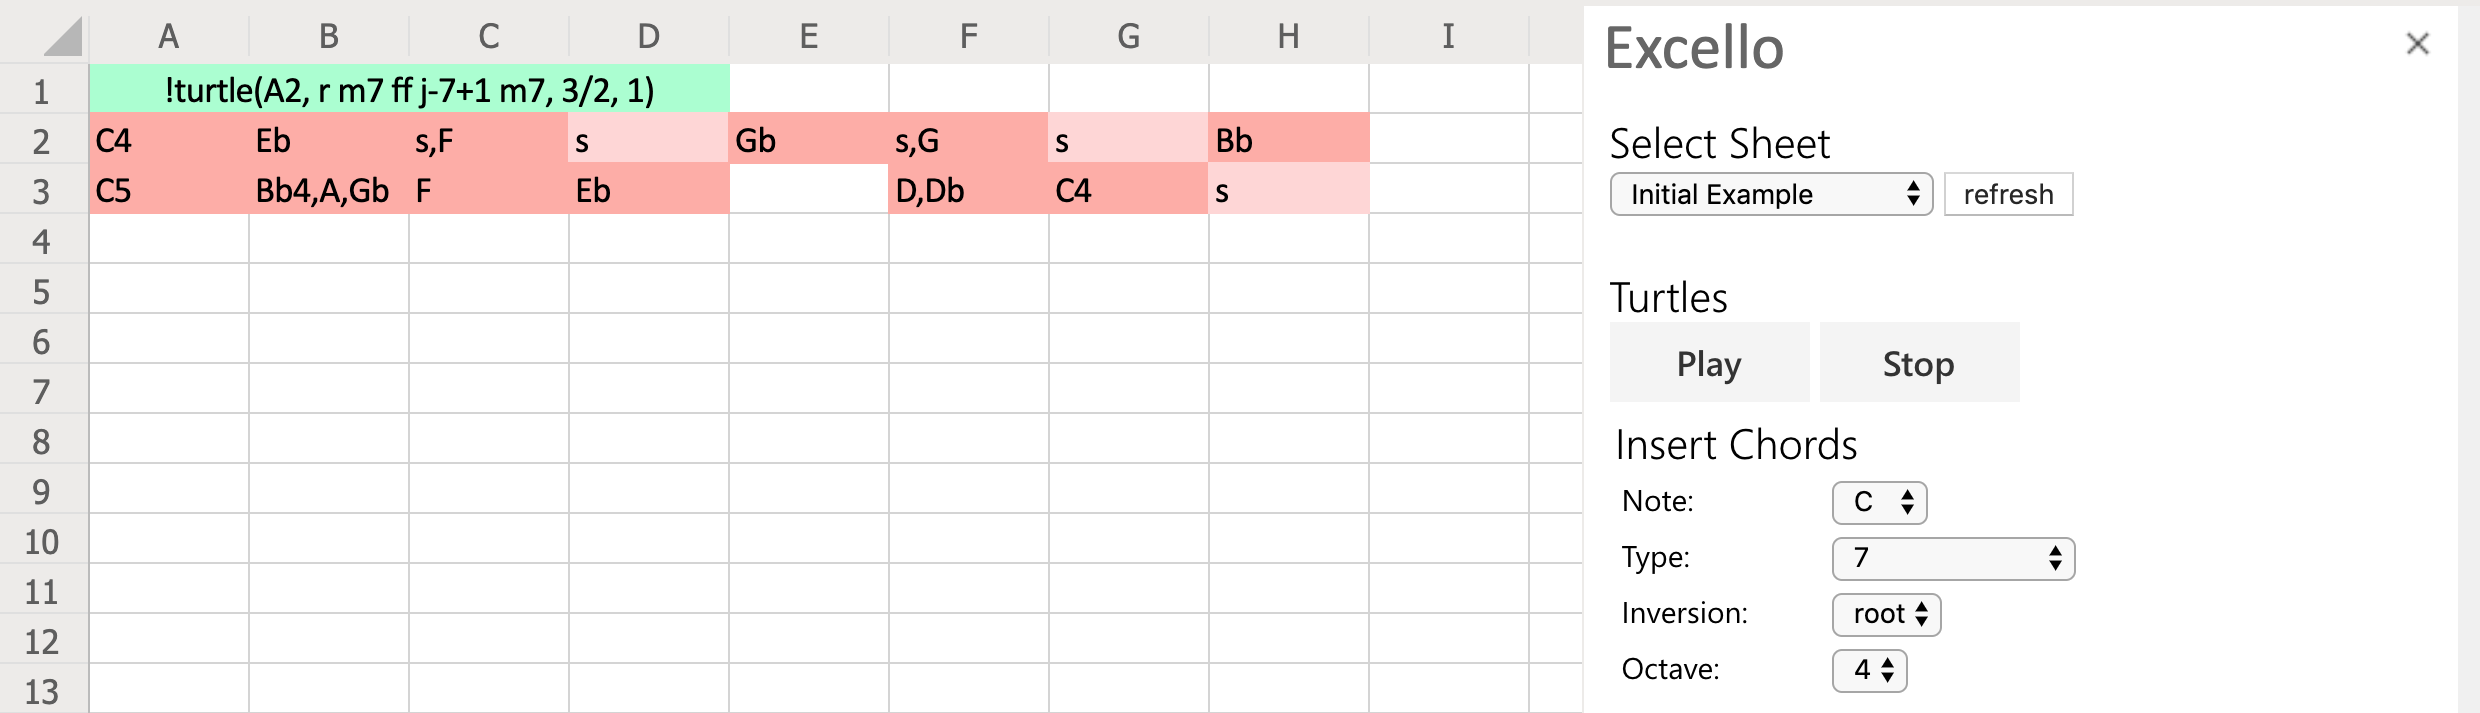
\includegraphics[width=150mm]{figs/initialPrototype.png}}
\caption{A two line motif defined in the initial Excello prototype}
\label{implementation:initialPrototype}
\end{figure}
\begin{figure}[tbh]
\centerline{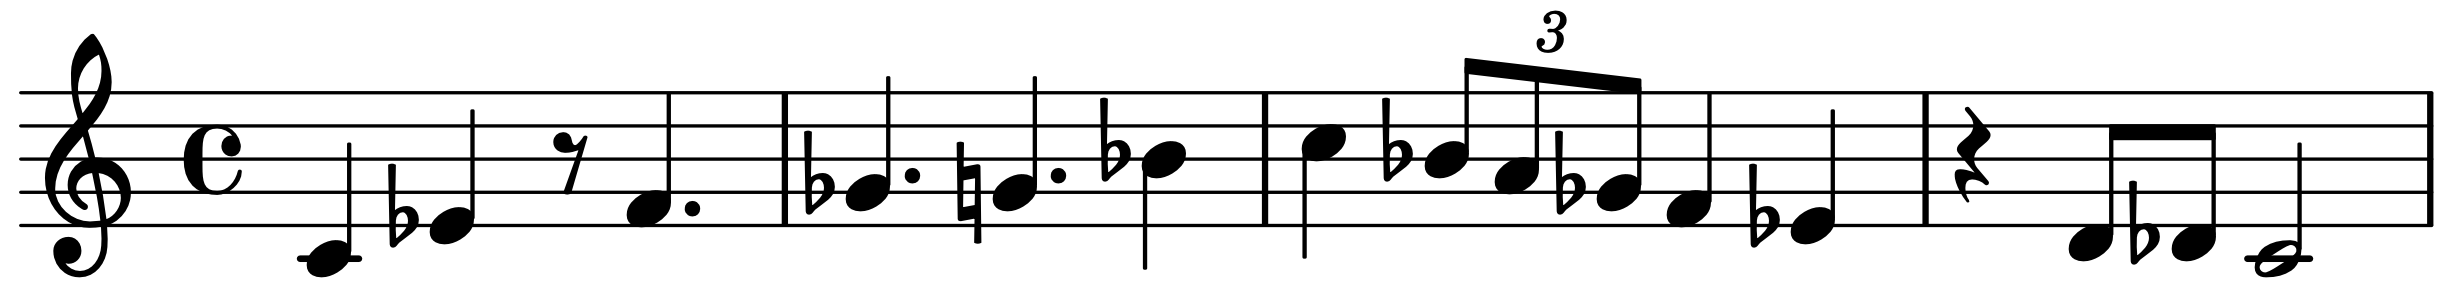
\includegraphics[width=150mm]{figs/initialScore.png}}
\caption{The notes played by the turtle in Figure \ref{implementation:initialPrototype}}
\label{implementation:initialScore}
\end{figure}

\vspace{-10pt}
\paragraph{} Notes and turtles can be defined in any cell. Turtles' interpretation of cells is shown in Table \ref{tab:cells}. When the Excello add-in is opened, a window opens on the right side of Excel as shown in Figure \ref{implementation:initialPrototype}. The melodic line produced is shown in figure \ref{implementation:initialScore}. Play and stop buttons launch all the turtles defined in the spreadsheet and initiate playback with a realistic piano sound.

\begin{table}[htb]
\centering
% \caption{Grammar Rules for the turtle movement instructions. $z \in \Z$}
\vspace{1pt}
\begin{tabular}{|l|l|} \hline
\textbf{Interpretation}&\textbf{Format}\\ \hline
Note& Name (A-G), optional accidental and octave number e.g.~\texttt{F$\sharp$4}\\ \hline
Sustain& \texttt{s}\\ \hline
Multiple notes& Notes, rests or sustains separated by a comma. Rests \\
subdivided in time& must be a space or an empty string e.g.~\texttt{E4,,C4,s}\\ \hline
Rest& Any cell not interpreted as a note, sustain or multi-note. \\ \hline
\end{tabular}
\caption{Interpretation of cells.\label{tab:cells}}
\end{table}

\subsection{Turtles}

\paragraph{} The following formula is enetered into a cell in the grid to define a turtle:\\
\texttt{!turtle(<Starting Cell>, <Movement>, <Speed>, <Number of Loops>)}

\vspace{-5pt}
\subsubsection{Activation}

\paragraph{} The prefix ``\texttt{!}" indicates the turtle will be activated when the play button is pressed. Just as digital audio workstations allow track muting and soloing, this can be used to modify which turtles play, without losing their definitions.

\vspace{-5pt}
\subsubsection{Starting Cell}

\paragraph{} The turtle's starting cell (\texttt{A2} in Figure \ref{implementation:initialPrototype}), which is also played, is a cell reference. As with Excel formulae, this is a concatenation of letters for the column and numbers for the row.

\paragraph{} As each turtle only plays one note at a time, multiple turtles must be defined to play polyphonic music such as chords. It was believed that users would define turtles following identical paths but in adjacent rows or columns. Multiple turtles following identical paths but starting from adjacent cells are defined using the existing Excel range notation for the starting cells. ``\texttt{A2:A5}" would define four turtles in the cells A2,A3,A4,A5. This prevents writing multiple turtle definitions differing in only the start cell row.

\vspace{-5pt}
\subsubsection{Movement}

\paragraph{} Turtles start facing north. The language for programming turtle movement is discussed in the Preparation chapter. The instructions are \texttt{r m7 ff j-7+1 m7} in Figure \ref{implementation:initialPrototype}. Using brackets to repeat movements had not been implemented by the start of the participatory design process.

\vspace{-5pt}
\subsubsection{Speed}

\paragraph{} An optional third argument is the speed of the turtle relative to 160 cells per minute. The default, 1, corresponds to 160 cells per minute. ``\texttt{3/2}", as in Figure \ref{implementation:initialPrototype}, would move the turtle at 240 cells per minute. Relative speed was used so it would be easier to tell the speed relation between turtles. This particularly suits phase music. Arbitrary maths can be provided, allowing turtles' speeds to be irrational multiples of each other.

\vspace{-5pt}
\subsubsection{Number of Loops}

\paragraph{} An optional fourth argument defines the number of repetitions of the turtle's entire path (\texttt{1} in Figure \ref{implementation:initialPrototype}). By default, the turtle loops infinitely. Repeating parts (e.g.~the cello in Pachelbel's Canon in D) therefore only need defining once.

\subsection{Highlighting}

\paragraph{} To assist recognising notes and turtles, when the play button is pressed, cells are highlighted. Activated or deactivated turtle definitions are highlighted green. Cells containing definitions of notes, or multiple notes, are highlighted red. Sustain cells are highlighted a lighter red, showing correspondence to notes whilst maintaining differentiation.

\subsection{Chord Input}

\paragraph{} To use the musical abstractions of chords whilst keeping the paradigm that a turtle is responsible for up to one note at any time, a tool to add chords is included. The note, type, inversion\footnote{Which note of the chord comes first, the other notes ascend from this. This is much like list rotations.} and starting octave of the chord are input into four drop-downs. The insert button enters the notes of the chord into the grid. If a single cell or a range taller than it is wide is highlighted in the spreadsheet, the notes are inserted vertically starting at the top-left of the range. Otherwise, the notes will be inserted horizontally. Whether the turtles are moving horizontally or vertically both chords and arpeggios\footnote{Where the notes of a chord are played individually in rising or descending order.} can be easily defined. Thus, helpful musical abstractions are still available whilst keeping the cleanness of the turtle system.

\section{Formative Evaluation}

\paragraph{} To guide development to best suit users, participants were involved in formative evaluation. Twenty-one University of Cambridge students, across a range of subjects, took part in the participatory design process. Initially, one-on-one tutorials on the initial prototype were given, followed by a short exercise. After these, users were interviewed on how they found Excello, drawing particular attention to actions that they found particularly unintuitive or requiring notable mental effort. Comparisons were made to musical interfaces with which participants were already familiar. The ethical and data handling procedures are discussed in the evaluation chapter.

\paragraph{} To realistically simulate how Excello would be used, participants carried out an exercise of their choice. Often this was transcribing a piece from memory or from traditional notation into the Excello notation. Two exercises were provided if participants had no immediate inspiration; transcribing a piece from western notation or changing existing Excello notation.

\paragraph{} These sessions were carried out in January 2019. Participants were asked to continue using Excello until the summative evaluation sessions in March. Additional feedback was collected as participants used Excello in their own time. This also ensured the summative evaluation was done with users that had sufficient experience of the interface.
% Participants were encouraged to get in contact with any additional issues or suggestions they had during this time.

\subsection{Issues and Suggestions}

\paragraph{} The issues and suggestions from the participatory design process are summarised below.

\subsubsection{Turtle Notation}

\paragraph{} Dynamics in the turtle instructions (e.g. \texttt{ppp m p m mf m ff m}) made establishing the turtle's path harder, as not all commands related to movement (``\texttt{m4}"). As the dynamics weren't next to the notes to which they corresponded, knowing the volume of a note or where to place the dynamics within the turtle to apply to notes in the spreadsheet was challenging. The initial prototype had no way to assign a dynamic to notes in the first cell. The starting cell could be empty, but this was inconvenient for looping parts, as this empty cell would be included in the loop. Users not familiar with western notation dynamics found them unintuitive. Furthermore, these discrete markings do not enable a continuous volume scale.

\paragraph{} When transcribing a piece, dividing its tempo by 160 for the relative speed caused unnecessary work. Users also forgot whether relative speed referred to the time spent in each cell or how quickly the turtle moved. Following the tutorial, users often had to check the position and meaning of turtle arguments.

\paragraph{} As the number of dynamics and movement commands grew, instructions became long and establishing turtle behaviour became cognitively challenging. Some users confused the ``\texttt{s}" within the turtle instructions to mean sustain (as it does in cells) and not south.

\subsubsection{Feedback}

\paragraph{} It was often unknown if pressing play actually registered, especially if the workbook saving delayed Excello's access to the spreadsheet. If a turtle had accidentally been left activated (with ``\texttt{!}"), the entire grid required searching to locate it. Users requested a summary of active turtle locations in addition to the highlighting.

\subsubsection{MIDI conversions}

\paragraph{} Users of production software said importing and exporting MIDI files would be helpful. If working with an existing MIDI file, converting that into the Excello notation would be convenient. Exportation would let Excello be used to create chord sequences, bass lines and the piece structure, before adding additional effects and recording in digital audio work stations.

\subsubsection{Sources of effort when writing}

\paragraph{} After inputting notes into the grid, the number of cells the turtle had to move required counting. As these were often in a straight line, the Excel status bar allowed users to select cells and immediately see how many there were. However, this was still not efficient, and was particularly inconvenient when users were writing notes and periodically testing what they had written so far. Some users instructed turtles to move forward significantly more steps than required to prevent counting. This is not feasible for looping parts. It was suggested that turtles could determine independently how far they should move.

\paragraph{} Instructions with repeated movements such as moving to the end of a line and jumping down to the beginning of a line below, required a lot of repetition.

\paragraph{} Many of the notes in melodic lines are frequently in the same octave. As such, repeatedly writing out the octave number was tiresome. One user made a comparison to LilyPond~\cite{sandberg:lily} where if the note length is not defined, the previous length would be used.

\paragraph{} Some users find it more intuitive to consider a melodic line by the intervals between notes rather than by the note names. A modulated\footnote{Where the pitch of every note in the sequence has moved by the same amount.} melody line required it to be written out again and could not be derived quicker any from the original version.

\subsubsection{Chords}

\paragraph{} Most users used a small subset of the available chord types, but had to find these within a large list. Separation of the more common chords was requested. Initially, notes inserted vertically had the lowest note at the top with pitch increasing down the column. Because higher pitch notes appear higher up the staff, it was suggested that inverting the order would be more intuitive. Initially, it was unclear what the different drop-downs corresponded to, with some users selecting the 7 from the octave number to try and insert a Maj7\footnote{A type of chord where the seventh note in the scale is added.} chord.

\subsubsection{Activation of Turtles}

\paragraph{} When toggling turtles' activations, entering the edit mode for each cell to add or remove the exclamation mark was very tedious.

\section{Second Prototype}

\paragraph{} Following the formative evaluation sessions and feedback, additions and modifications were made to solve the problems and opportunities that arose.

\subsection{Dynamics}

\paragraph{} To help extract a turtle's path and establish notes' volumes, dynamics are instead now inserted in the cells after the note, separated by a space as in Manhattan~\cite{nash:manhattan}. As before, this will apply to all following notes, until the volume is redefined. A single turtle definition with multiple start cells can now play parts of different volume. However, notes in the grid can be limited to only playing at their given volume. To play the same notes at a different volume, a new path must be made. Overall, the new system was believed to be preferable.

\paragraph{} To use a continuous volume scale, in addition to existing dynamic symbols, a number between 0 and 1 can instead be provided where 0 is silent and 1 is equivalent to \texttt{fff}.

\subsection{Nested Instructions}

\paragraph{} Nested instructions with repeats reduce turtle instructions and more easily incorporate repeated sections or movements. Multiple commands placed within parentheses followed by a number are repeated that number of times. Whilst the fourth argument of the turtle repeats the turtle's entire musical output, repetitions within the movement instructions allow paths to be defined more concisely.

\subsection{Absolute Tempo}

\paragraph{} The turtle's speed is now defined by cells per minute, rather than the relative value used initially. However, values less than 10 are interpreted in the original relative way for backwards compatibility with participants' existing work. To maintain consistency in a production version, this will be removed so speed must be defined absolutely. As speed and dynamics are different orders of magnitude, confusion between them is reduced.

\subsection{Custom Excel Functions}

\paragraph{} Two custom Excel functions have been implemented to aid composition. One to define turtles and a second to transpose notes. This allows Excello to take advantage of the functionality of the existing Excel ecosystem; drag-fill, autocomplete, cell referencing, etc.

\vspace{-20pt}
\texttt{\subsubsection{EXCELLO.TURTLE}}

\paragraph{} When writing a formula, a prompt informs users of the position of arguments, and whether they are optional. This outputs the turtle definition as text. All turtles could reference a single cell for their speeds. Relative tempi could then be implemented by the speed argument of each turtle being a multiple of this global speed as shown in Figure \ref{implementation:turtleFunction}.

\begin{figure}[tbh]
\centerline{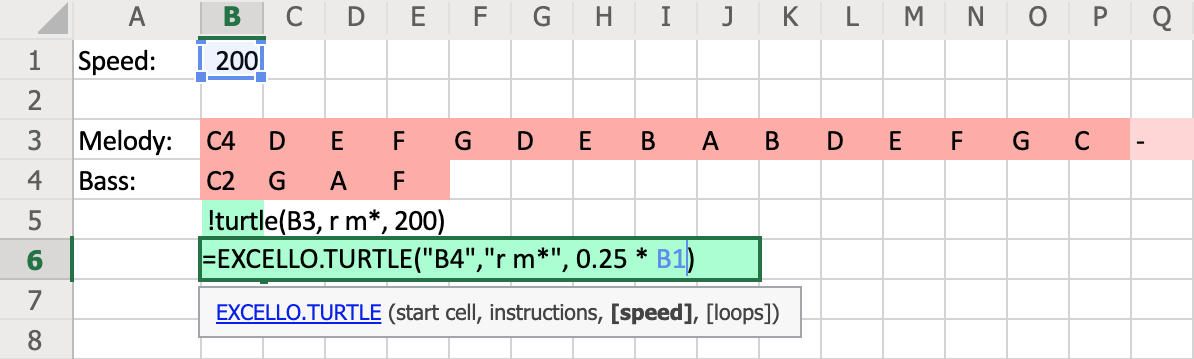
\includegraphics[width=150mm]{figs/turtleFunction.png}}
\caption{Defining a turtle using the \texttt{EXCELLO.TURTLE} function.}
\label{implementation:turtleFunction}
\end{figure}

\vspace{-30pt}
\texttt{\subsubsection{EXCELLO.MODULATE}}

\paragraph{} A modulating function lets melodic lines be defined by the intervals between notes and provides easy modulation of existing sections of a piece. The function takes a cell and an interval and outputs the cell with any notes transposed by the interval, maintaining any dynamics. A section can be modulated by calling this function on the first note with a provided interval and then using drag-fill. By using the previous note and one of a series of intervals as the arguments, a melodic line can quickly be produced from a starting note and a series of intervals as shown in Figure \ref{implementation:modulateFunction}.

\begin{figure}[tbh]
\centerline{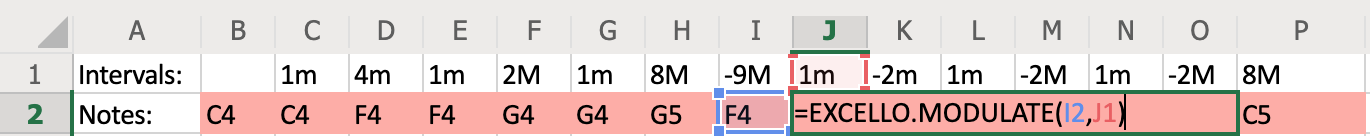
\includegraphics[width=150mm]{figs/modulateFunction.png}}
\caption{Transposing notes using the \texttt{EXCELLO.MODULATE} function.}
\label{implementation:modulateFunction}
\end{figure}

%  \ref{examples}

\subsection{Sustain}

\paragraph{} To prevent confusion between the south instruction and sustains. The symbol ``\texttt{-}" sustains a note. This was chosen because it is light and also has some similarity to a tie.\footnote{A line used in musical notation to increase the length of a note by joining it to another note.} Again, to maintain backwards compatibility, ``\texttt{s}" in a cell is still interpreted as a sustain.

\subsection{Active Turtles}

\paragraph{} To show that active turtle definitions have been recognised, a list of locations of the active turtles is given below the play button. This also helps find spurious turtles not intended to be activated.

\subsection{Automatic Movement}

\paragraph{} To prevent counting the cells in a line, \texttt{m*} instructs a turtle to move as far as there are notes or sustains defined in the direction it is facing. After adding more notes, the turtle instructions do not need editing before pressing play. A part may be meant to finish with a number of rests. As rests are notated with blank cells, a method to extend the path to include these rests was required. A cell can be explicitly defined as a rest with ``\texttt{.}". This is required if multiple turtles are playing a repeating section where one turtle's final cell as a note, sustain or multi-note cell. Without an explicit rest, the turtle would repeat too soon and the parts would consequently be out of phase.

\subsection{Inferred Octave}

\paragraph{} Octave numbers are inferred if omitted. Two methods were considered. Firstly, as most intervals within melodic lines are small, the nearest note could be played.
% This means that a scale would only need the octave defining in the first note.
Whilst this may require the fewest explicit statements of octave numbers, it would be hard to immediately identify the octave of any given note. The last defined octave in the path would need finding and then all subsequent notes walked through keeping track of the octave. The second consideration was to always use the last defined octave. Whilst this may require many octave definitions around the boundary between octaves, it is easier to find the octave of a note by backtracking. The second option was therefore implemented.

\subsection{Chords}

\paragraph{} To aid entering common chords, common types are repeated in a section at the top of the type drop-down. The chord drop-downs layout has been improved with labels to make it clearer what the values refer to. If the notes were entered vertically, the order was reversed, increasing correspondence with traditional staff notation.

\subsection{Activation of turtles}

\paragraph{} A ``Toggle Activation" button was added to the add-in window. When a cell or range is highlighted in the spreadsheet, the activation of any turtle definitions in this range will be toggled when the button is pressed.  This significantly decreases the time to toggle activations, as only two clicks are required, rather than entering the cell edit mode to add or remove an exclamation mark.

\section{Final Prototype Implementation}

\paragraph{} This section discusses the underlying implementation of the final prototype, following the participatory design. Excello consists of three main parts: the turtle system for playing the grid contents, the chord input tool, and the custom Excel functions.

\paragraph{} When the play button is pressed, turtle definitions in the grid are identified. For each, the starting cell and movement instructions are used to establish the contents of the cells it passes through. This is converted to a series of note definitions - pitch, start time, duration, volume. The speed and loop parameters are used to create the structure interpreted by the Tone.js library to schedule and initiate playback. An overview of the data flow and subtasks required to create the musical playback is shown in Figure \ref{fig:overview}.

\begin{figure}[htb]
\begin{center}
  
  \tikzset{every picture/.style={line width=0.75pt}} %set default line width to 0.75pt

  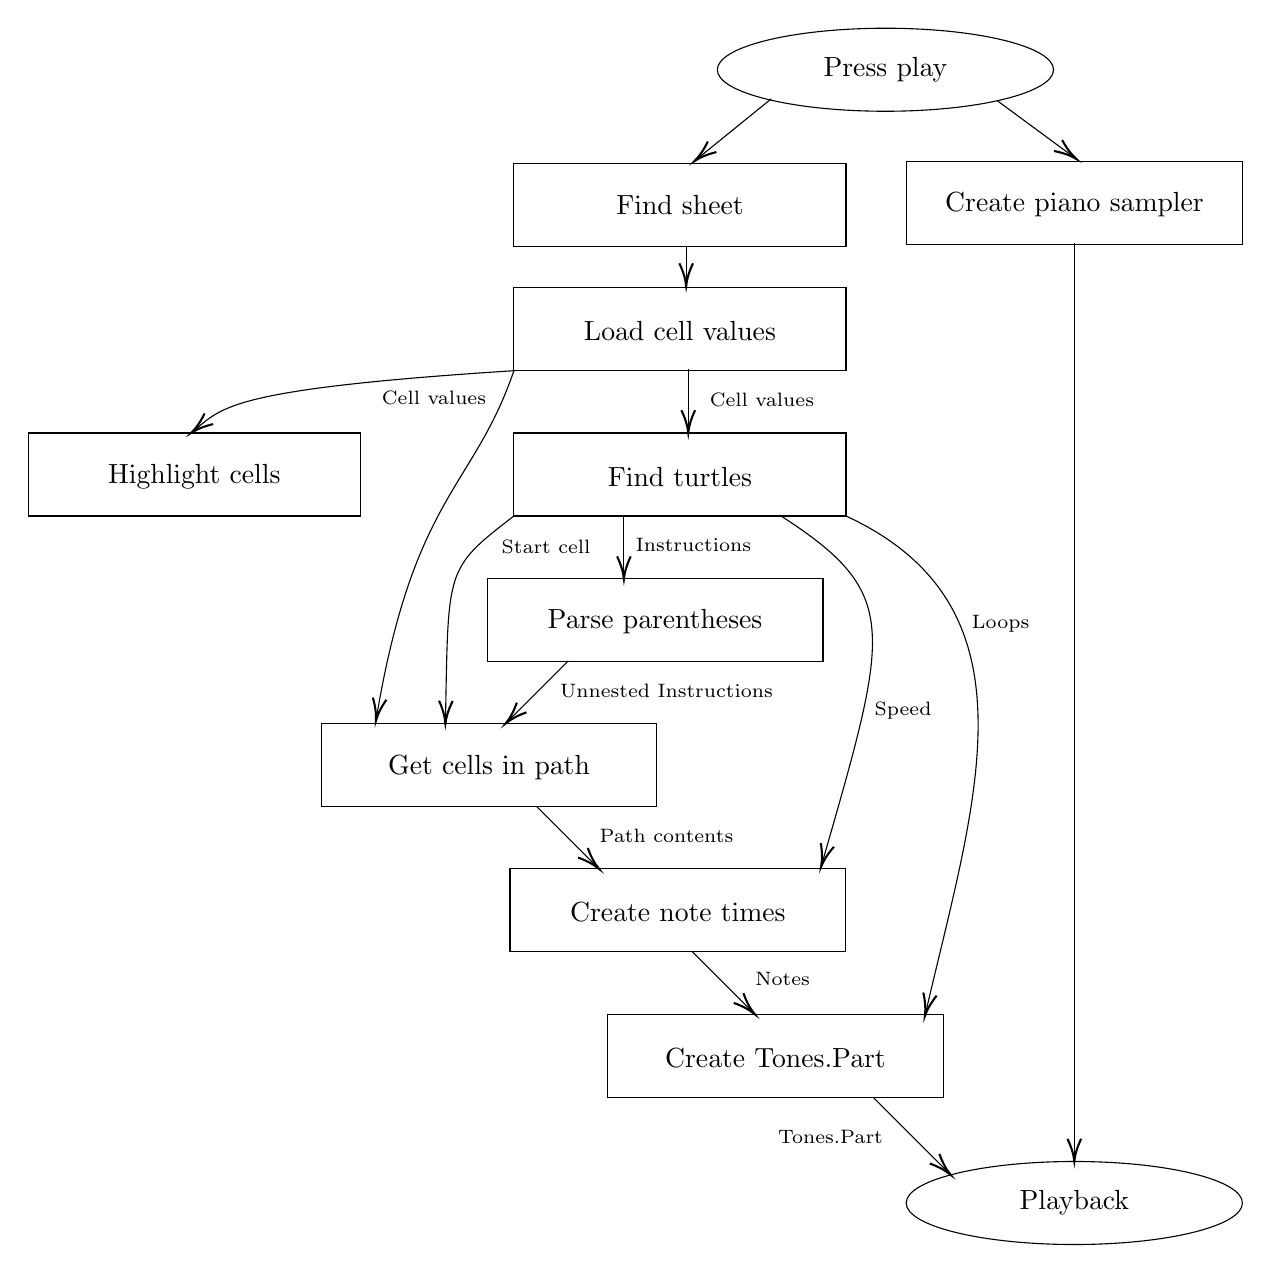
\begin{tikzpicture}[x=0.75pt,y=0.75pt,yscale=-1,xscale=1]
  %uncomment if require: \path (0,604); %set diagram left start at 0, and has height of 604

  %Shape: Rectangle [id:dp3390223975782729]
  \draw   (244.5,71) -- (404.5,71) -- (404.5,111) -- (244.5,111) -- cycle ;

  %Shape: Rectangle [id:dp7168559924493858]
  \draw   (244.5,131) -- (404.5,131) -- (404.5,171) -- (244.5,171) -- cycle ;

  %Shape: Rectangle [id:dp8835932361497658]
  \draw   (433.7,70) -- (595.5,70) -- (595.5,110) -- (433.7,110) -- cycle ;

  %Shape: Rectangle [id:dp9464422191216635]
  \draw   (244.5,201) -- (404.5,201) -- (404.5,241) -- (244.5,241) -- cycle ;

  %Shape: Rectangle [id:dp6384624480751633]
  \draw   (231.6,271) -- (393.4,271) -- (393.4,311) -- (231.6,311) -- cycle ;

  %Shape: Rectangle [id:dp2927464084046889]
  \draw   (151.6,341) -- (313.4,341) -- (313.4,381) -- (151.6,381) -- cycle ;

  %Shape: Rectangle [id:dp9052659554068596]
  \draw   (242.6,411) -- (404.4,411) -- (404.4,451) -- (242.6,451) -- cycle ;

  %Shape: Rectangle [id:dp5637329489183025]
  \draw   (289.6,481) -- (451.4,481) -- (451.4,521) -- (289.6,521) -- cycle ;

  %Curve Lines [id:da3917180624639185]
  \draw    (244.5,241) .. controls (211.17,266.67) and (212.98,265.81) .. (211.52,339.88) ;
  \draw [shift={(211.5,341)}, rotate = 271.14] [color={rgb, 255:red, 0; green, 0; blue, 0 }  ][line width=0.75]    (10.93,-3.29) .. controls (6.95,-1.4) and (3.31,-0.3) .. (0,0) .. controls (3.31,0.3) and (6.95,1.4) .. (10.93,3.29)   ;

  %Straight Lines [id:da6961662223442007]
  \draw    (297.5,241) -- (297.5,269.4) ;
  \draw [shift={(297.5,271.4)}, rotate = 270] [color={rgb, 255:red, 0; green, 0; blue, 0 }  ][line width=0.75]    (10.93,-3.29) .. controls (6.95,-1.4) and (3.31,-0.3) .. (0,0) .. controls (3.31,0.3) and (6.95,1.4) .. (10.93,3.29)   ;

  %Curve Lines [id:da9168950950169605]
  \draw    (372.6,240.6) .. controls (431.31,278.41) and (425.56,294.84) .. (392.99,408.28) ;
  \draw [shift={(392.5,410)}, rotate = 286.01] [color={rgb, 255:red, 0; green, 0; blue, 0 }  ][line width=0.75]    (10.93,-3.29) .. controls (6.95,-1.4) and (3.31,-0.3) .. (0,0) .. controls (3.31,0.3) and (6.95,1.4) .. (10.93,3.29)   ;

  %Curve Lines [id:da7972588626438504]
  \draw    (404.5,241) .. controls (499.03,284.78) and (466.83,377.07) .. (442.86,480.44) ;
  \draw [shift={(442.5,482)}, rotate = 282.99] [color={rgb, 255:red, 0; green, 0; blue, 0 }  ][line width=0.75]    (10.93,-3.29) .. controls (6.95,-1.4) and (3.31,-0.3) .. (0,0) .. controls (3.31,0.3) and (6.95,1.4) .. (10.93,3.29)   ;

  %Straight Lines [id:da6822022155717844]
  \draw    (270.7,310.8) -- (241.91,339.59) ;
  \draw [shift={(240.5,341)}, rotate = 315] [color={rgb, 255:red, 0; green, 0; blue, 0 }  ][line width=0.75]    (10.93,-3.29) .. controls (6.95,-1.4) and (3.31,-0.3) .. (0,0) .. controls (3.31,0.3) and (6.95,1.4) .. (10.93,3.29)   ;

  %Straight Lines [id:da4884596231580207]
  \draw    (255.5,381) -- (284.09,409.59) ;
  \draw [shift={(285.5,411)}, rotate = 225] [color={rgb, 255:red, 0; green, 0; blue, 0 }  ][line width=0.75]    (10.93,-3.29) .. controls (6.95,-1.4) and (3.31,-0.3) .. (0,0) .. controls (3.31,0.3) and (6.95,1.4) .. (10.93,3.29)   ;

  %Straight Lines [id:da9233366942734922]
  \draw    (330.5,451) -- (359.09,479.59) ;
  \draw [shift={(360.5,481)}, rotate = 225] [color={rgb, 255:red, 0; green, 0; blue, 0 }  ][line width=0.75]    (10.93,-3.29) .. controls (6.95,-1.4) and (3.31,-0.3) .. (0,0) .. controls (3.31,0.3) and (6.95,1.4) .. (10.93,3.29)   ;

  %Straight Lines [id:da3670498457872964]
  \draw    (417.5,521) -- (453.49,556.99) ;
  \draw [shift={(454.9,558.4)}, rotate = 225] [color={rgb, 255:red, 0; green, 0; blue, 0 }  ][line width=0.75]    (10.93,-3.29) .. controls (6.95,-1.4) and (3.31,-0.3) .. (0,0) .. controls (3.31,0.3) and (6.95,1.4) .. (10.93,3.29)   ;

  %Straight Lines [id:da28794703530347365]
  \draw    (327.5,111) -- (327.5,128.2) ;
  \draw [shift={(327.5,130.2)}, rotate = 270] [color={rgb, 255:red, 0; green, 0; blue, 0 }  ][line width=0.75]    (10.93,-3.29) .. controls (6.95,-1.4) and (3.31,-0.3) .. (0,0) .. controls (3.31,0.3) and (6.95,1.4) .. (10.93,3.29)   ;

  %Straight Lines [id:da33376731250782754]
  \draw    (328.5,170) -- (328.5,199) ;
  \draw [shift={(328.5,201)}, rotate = 270] [color={rgb, 255:red, 0; green, 0; blue, 0 }  ][line width=0.75]    (10.93,-3.29) .. controls (6.95,-1.4) and (3.31,-0.3) .. (0,0) .. controls (3.31,0.3) and (6.95,1.4) .. (10.93,3.29)   ;

  %Curve Lines [id:da2676626927985757]
  \draw    (244.5,171) .. controls (225.1,227.72) and (196.29,230.77) .. (178.27,338.17) ;
  \draw [shift={(178,339.8)}, rotate = 279.38] [color={rgb, 255:red, 0; green, 0; blue, 0 }  ][line width=0.75]    (10.93,-3.29) .. controls (6.95,-1.4) and (3.31,-0.3) .. (0,0) .. controls (3.31,0.3) and (6.95,1.4) .. (10.93,3.29)   ;

  %Straight Lines [id:da024649031996502035]
  \draw    (514.5,109.6) -- (514.5,550) ;
  \draw [shift={(514.5,552)}, rotate = 270] [color={rgb, 255:red, 0; green, 0; blue, 0 }  ][line width=0.75]    (10.93,-3.29) .. controls (6.95,-1.4) and (3.31,-0.3) .. (0,0) .. controls (3.31,0.3) and (6.95,1.4) .. (10.93,3.29)   ;

  %Shape: Ellipse [id:dp13505581605963868]
  \draw   (433.5,572) .. controls (433.5,560.95) and (469.76,552) .. (514.5,552) .. controls (559.24,552) and (595.5,560.95) .. (595.5,572) .. controls (595.5,583.05) and (559.24,592) .. (514.5,592) .. controls (469.76,592) and (433.5,583.05) .. (433.5,572) -- cycle ;

  %Shape: Ellipse [id:dp006287630832967794]
  \draw   (342.5,26) .. controls (342.5,14.95) and (378.76,6) .. (423.5,6) .. controls (468.24,6) and (504.5,14.95) .. (504.5,26) .. controls (504.5,37.05) and (468.24,46) .. (423.5,46) .. controls (378.76,46) and (342.5,37.05) .. (342.5,26) -- cycle ;

  %Straight Lines [id:da09048722077694915]
  \draw    (368.5,40) -- (333.05,68.74) ;
  \draw [shift={(331.5,70)}, rotate = 320.96000000000004] [color={rgb, 255:red, 0; green, 0; blue, 0 }  ][line width=0.75]    (10.93,-3.29) .. controls (6.95,-1.4) and (3.31,-0.3) .. (0,0) .. controls (3.31,0.3) and (6.95,1.4) .. (10.93,3.29)   ;

  %Straight Lines [id:da9578993167654264]
  \draw    (477.5,41) -- (513.89,67.81) ;
  \draw [shift={(515.5,69)}, rotate = 216.38] [color={rgb, 255:red, 0; green, 0; blue, 0 }  ][line width=0.75]    (10.93,-3.29) .. controls (6.95,-1.4) and (3.31,-0.3) .. (0,0) .. controls (3.31,0.3) and (6.95,1.4) .. (10.93,3.29)   ;

  %Shape: Rectangle [id:dp25073410390478523]
  \draw   (10.5,201) -- (170.5,201) -- (170.5,241) -- (10.5,241) -- cycle ;

  %Curve Lines [id:da2454539812308738]
  \draw    (244.5,171) .. controls (108.92,179.69) and (104.17,188.37) .. (90.53,199.75) ;
  \draw [shift={(89,201)}, rotate = 321.34000000000003] [color={rgb, 255:red, 0; green, 0; blue, 0 }  ][line width=0.75]    (10.93,-3.29) .. controls (6.95,-1.4) and (3.31,-0.3) .. (0,0) .. controls (3.31,0.3) and (6.95,1.4) .. (10.93,3.29)   ;


  % Text Node
  \draw (324.5,91) node  [align=left] {Find sheet};
  % Text Node
  \draw (324.5,152) node  [align=left] {Load cell values};
  % Text Node
  \draw (514.6,91) node  [align=left] {Create piano sampler};
  % Text Node
  \draw (324.5,222) node  [align=left] {Find turtles};
  % Text Node
  \draw (312.5,292) node  [align=left] {Parse parentheses};
  % Text Node
  \draw (232.5,362) node  [align=left] {Get cells in path};
  % Text Node
  \draw (323.5,432) node  [align=left] {Create note times};
  % Text Node
  \draw (370.5,502) node  [align=left] {Create Tones.Part};
  % Text Node
  \draw (514.5,572) node [] [align=left] {\textcolor[rgb]{0,0,0}{Playback}};
  % Text Node
  \draw (260,256) node  [align=left] {{\scriptsize Start cell}};
  % Text Node
  \draw (331,255) node  [align=left] {{\scriptsize Instructions}};
  % Text Node
  \draw (432,335) node  [align=left] {{\scriptsize Speed}};
  % Text Node
  \draw (479,293) node  [align=left] {{\scriptsize Loops}};
  % Text Node
  \draw (318,325) node  [align=left] {{\scriptsize Unnested Instructions}};
  % Text Node
  \draw (318,395) node  [align=left] {{\scriptsize Path contents}};
  % Text Node
  \draw (374,464) node  [align=left] {{\scriptsize Notes}};
  % Text Node
  \draw (397,540) node  [align=left] {{\scriptsize Tones.Part}};
  % Text Node
  \draw (206,184) node  [align=left] {{\scriptsize Cell values}};
  % Text Node
  \draw (423.5,26) node [] [align=left] {Press play};
  % Text Node
  \draw (364,185) node  [align=left] {{\scriptsize Cell values}};
  % Text Node
  \draw (90.5,222) node  [align=left] {Highlight cells};


  \end{tikzpicture}

\end{center}
\caption{An overview of the playback algorithm and dataflow of Excello\label{fig:overview}}
\end{figure}

\paragraph{} The \texttt{Sampler} is an extension of the \texttt{Tone.Instrument} class. This interpolates between pitched samples to create arbitrary notes. A sampler is loaded using the Salamander grand piano samples~\footnote{https://freepats.zenvoid.org/Piano/acoustic-grand-piano.html} which includes four pitches (out of a possible 12) per octave. This accurately interpolates notes whilst reducing loading times and storage requirements.

\subsection{Identifying Cells}

\paragraph{} A drop-down is populated with names loaded using the Office API. Having pressed play, the cell values from the selected sheet are loaded and then analysed for highlighting and calculating the musical output. Cells containing at least one note definition are highlighted red. A note must contain a note name, optional accidental, optional octave number, and optional volume instruction following a space. This is a dynamic marking or number between 0 and 1. Notes are identified using the following regular expression:

\begin{verbatim}
^[A-G](#|b|)?[1-9]?( (0(\.\[0-9]+)?|1(\.0)?|ppp|pp|p|mp|mf|f|ff|fff))?$
\end{verbatim}

\paragraph{} Cells containing multiple definitions (e.g. ``\texttt{C4 ff,-, ,D}", ``\texttt{,,G,F$\sharp$}") are split using commas. The resulting strings are trimmed of starting and ending whitespace and then must either be a note, sustain (``\texttt{-}" or ``\texttt{s}"), explicit rest (``\texttt{.}") or empty string (created from trimming a rest). Cells matching ``\texttt{-}",``\texttt{.}" or ``\texttt{s}" are highlighted a lighter red. Turtle definitions (e.g. ``\texttt{!turtle(B2:B4, r m*, 200, 1)}") are identified using:
\begin{verbatim}
^(!turtle\().*(\))$
\end{verbatim}
and these cells are highlighted green. The addresses of cells containing a turtle definition are added to the live turtle section of the add-in window.

\subsection{Parsing Movement Instructions}

\paragraph{} Movement instructions are converted to a single unnested list of commands (e.g.~``\texttt{(r m2)2}" becomes ``\texttt{[r, m2, r, m2]}") so the turtle's path can be established. The \texttt{parse} method of the Parenthesis\footnote{https://www.npmjs.com/package/parenthesis} library seemed suitable for aiding this string manipulation. This parses strings containing brackets into a nested array. For example, \texttt{parse(\textcolor[rgb]{0,0.7,0}{\upquote{a(b[c\{d\}])}})} gives \texttt{[\textcolor[rgb]{0,0.7,0}{\upquote{a(}}, [\textcolor[rgb]{0,0.7,0}{\upquote{b[}}, [\textcolor[rgb]{0,0.7,0}{\upquote{c\{}}, [\textcolor[rgb]{0,0.7,0}{\upquote{d}}], \textcolor[rgb]{0,0.7,0}{\upquote{\}}}], \textcolor[rgb]{0,0.7,0}{\upquote{]}}], \textcolor[rgb]{0,0.7,0}{\upquote{)}}]}.

\paragraph{} This suggests the string ``\texttt{(r m2)2}" would become \texttt{[\upquote{(}, [\upquote{r m2}], \upquote{)2}]}. By removing the brackets from these strings, a simple recursive method could be built to output \texttt{\upquote{r m2 r m2}} from \texttt{[[\upquote{r m2}], \upquote{2}]}. However, upon testing this, the library outputted an undefined array. From investigating the source code, I established that strings with a number following a closing parenthesis all produced this error. Substituting characters for the numbers or placing a symbol before all numbers and then later removing these would allow the library to be used. Instead, using the Parenthesis method as inspiration, I implemented my own parsing function tailored to Excello.

\paragraph{} This has two main steps. First, the deepest bracketed expression is stored in an array with the brackets removed. This expression is replaced in the original string with the string \upquote{\texttt{\_\_\_}$x$\texttt{\_\_\_}} where $x$ is the expression's index in the array. This is repeated until the string contains no brackets. Then a recursive function uses the values of $x$ to reconstruct the string in the nested array format. This method is outlined in Algorithm \ref{alg:parenthesis}. The Typescript implementation is in Appendix \ref{appendix:parseBrackets}.

\begin{algorithm}[!htp]
\caption{Parsing bracketed expression. \texttt{str.replace(regex,f)} (line 13) performs \texttt{f(s)} on the first substring, \texttt{s}, of \texttt{str} matching the regular expression \texttt{regex}.}
\label{alg:parenthesis}
\begin{algorithmic}[1]
\Procedure{parseBrackets}{$str$}

   \State $idPadding\gets \texttt{\upquote{\_\_\_}}$
   \State $unnestedStr\gets []$
   \State $deepestLevelBracketsRE\gets \texttt{RegExp(\upquote{\textbackslash\textbackslash([\^{}\textbackslash\textbackslash(\textbackslash\textbackslash)]*\textbackslash\textbackslash)})}$
   \State $replacementIDRE\gets \texttt{RegExp(\upquote{\textbackslash\textbackslash} + }idPadding\texttt{ + \upquote{([0-9]+)} + }idPadding\texttt{)}$\\

   \Procedure{replaceDeepestBracket}{$x$}
     \State \texttt{unnestedStr.push(x.substring(1, x.length-1))}
     \State \texttt{\textbf{return} idPadding + (unnestedStr.length - 1) + idPadding}
   \EndProcedure \\

   \While{\texttt{deepestLevelBracketsRE.test(str)}}
     \State \texttt{str = str.replace(deepestLevelBracketsRE,replaceDeepestBracket)}
   \EndWhile

   \State \texttt{unnestedStr[0] = str}\\

   \Procedure{reNest}{$outerStr$}
     \State $renestingStr\gets []$
     \While{There is a match of $replacementIDRE$ in $outerStr$}
       \State $matchIndex\gets$ index of the match in $outerStr$
       \State $matchID\gets$ ID of the match (number between padding)
       \State $matchString\gets$ matched string\\

       \If{$matchIndex >$ 0}
				\State $renestingStr$.push($outestStr$.substring(0, $matchIndex$))
			\EndIf
			\State $renestingStr$.push(reNest($unnestedStr$[$firstMatchID$]))
			\State $outestStr$ = $outestStr$.substring($matchIndex$ + $matchString$.length)
     \EndWhile
     \State $renestingStr$.push($outestStr$)
     \State \textbf{return} $renestingStr$
   \EndProcedure \\

   \State \textbf{return} \textsc{reNest}($unnestedStr$[0])

\EndProcedure
\end{algorithmic}
\end{algorithm}


\paragraph{} Having submitted a bug report on the Parenthesis GitHub, and implemented my own method for parsing turtle movement instructions, I implemented a fix to the Parenthesis library. The library previously performed replacements with the string \upquote{\texttt{\_\_\_}$x$}. $x$ and following numbers would concatenate forming a single number, causing the library to fail. My method of having an identifier before and after $x$ fixed this issue. I also added additional tests to Parenthesis to verify my method and ensure that previous tests all passed before submitting a pull request. I have made an open source contribution, as this has since been merged into the library and published.

\paragraph{} I wrote an additional recursive method to unnest the array into a single stream of commands. An empty string, \texttt{s}, is initialised. For each item in the array, if it is an array, unnest the contents recursively and add the result to s. If not, it will be one or more single movement commands. If the single movement commands start with a number, the result is added to \texttt{s} that number of times. The remaining instructions are added to \texttt{s}. This is outlined in Algorithm \ref{alg:unnest}. The implementation is shown in Appendix \ref{appendix:processParsedBrackets}.

\begin{algorithm}[!htbp]
\caption{Unnesting parsed bracketed expressions.}
\label{alg:unnest}
\begin{algorithmic}[1]
\Procedure{processParsedBrackets}{$arr$}

   \State $s\gets \texttt{\upquote{}}$
   \State $previousArr$

   \For{$v$ in $s$}
    \If{$v$ is an array}
     \State $previousArr \gets$ processParsedBrackets($v$)
    \Else
       \If{previous instruction was an array}
        \State $s \gets s + previousArr$
        \If{next instruction is a number}
          \State $s \gets s + previousArr$, that number of times minus one
        \EndIf
       \EndIf
       \State $s \gets s + $ remaining instruction in $v$
    \EndIf
   \EndFor
   \State \textbf{return} $s$

\EndProcedure
\end{algorithmic}
\end{algorithm}

\subsection{Getting Cells in Turtles' Paths}

\paragraph{} If the turtle's first argument defines a range of starting cells, the cell addresses of this range are calculated. For each starting cell, the unnested instructions and sheet values are used to find the contents of the cells the turtle passes through. This process models the movement of the turtle within the grid, keeping track of its position and the direction in which it is facing. For each instruction, the position and direction are updated as required, and the contents of any new cells entered are added to a list of notes.

\paragraph{} For the ``\texttt{m*}" instruction, the number of steps the turtle takes must be computed. Given the turtle's current position and direction, the one-dimensional array of cells in front of it is taken. The turtle should step to the last cell that defines a note, sustain or explicit rest. The number of steps is the array's length minus the index of the first element in the reversed array satisfying this criterion.

\subsection{Creating Note Times}

\paragraph{} The cells a turtle moves through are used to create a data structure containing the information for playback using the Tone library. For each turtle, the following array is produced: \texttt{[[<Note 1>,...,<Note N>], <number of cells>]} (note sequence array). Each note is as follows: \texttt{[<start time>, [<pitch>, <duration>, <volume>]]}. Volume and octave are added to each note if they were omitted from a cell.

\paragraph{} The Tone Transport is a timeline along which events can be scheduled. This supports many different representations of time. I used Transport Time for all note onsets and durations. This is of the form \texttt{\upquote{BARS:QUARTERS:SIXTEENTHS}} where the three values are numbers and can be non-integer. With \texttt{QUARTERS} representing the number of cells, the calculation of exact times, or arbitrary musical notes can be avoided. This allows the contents of cells to be easily converted to times to be interpreted by the Tones library.

\paragraph{} The note sequence array is initiated by counting the notes that are defined in the cell contents using regular expressions for identifying notes and multi-note cells. The cells are iterated through keeping track of the active note and adding it to the note sequence when it ends. Outside of this loop, variables track how many cells and notes through the process the algorithm is and whether it is currently a rest or note. Variables keep track of the note currently being played - when it started (\texttt{currentStart}), the pitch (\texttt{currentNote}) and the volume (\texttt{currentVolume}). As volume and octave number may be omitted, variables also keep track of these. Table \ref{tab:times} outlines the actions performed when a cell is read. Notes are added to the note sequence in the form \texttt{[currentStart, [currentNote, \upquote{0:} + noteLength + \upquote{:0}, currentVolume]]}.

\begin{table}[ht]
\begin{tabular}{|l|l|l|l|l|}
  \hline
  \textbf{Cell}&\textbf{State}&\multicolumn{3}{c|}{\textbf{Action}} \\
  \hline
  \multirow{5}{*}{Note}&\multirow{3}{*}{Note}&Note, octave and &Previous note added&currentStart = \\
  &&volume established&to note sequence&\upquote{0:}+beatCount+\upquote{:0}\\
  &&from cell contents&&currentNote = value\\
  \cline{2-2}
  \cline{4-4}
  &\multirow{2}{*}{Rest}&and previous values&inRest = false&noteLength = 1\\
  &&&&currentVolume = volume\\
  \hline
  \multirow{2}{*}{Sustain}&Note&\multicolumn{3}{l|}{noteLength++}\\
  \cline{2-5}
  &Rest&\multicolumn{3}{l|}{Nothing (has no semantic value)}\\
  \hline
  \multirow{3}{*}{Rest}&\multirow{2}{*}{Note}&\multicolumn{3}{l|}{Previous note added to note sequence}\\
  &&\multicolumn{3}{l|}{inRest = true}\\
  \cline{2-5}
  &Rest&\multicolumn{3}{l|}{Nothing}\\
  \hline
\end{tabular}
\caption{The actions taken when processing each cell to create note times. The beat count corresponds to the cell number being processed and is incremented each time.\label{tab:times}}
\end{table}
\vspace{-10pt}

\paragraph{} The same method is used for multi-note cells, except the note length and cell count are incremented by the appropriate fraction for each item in the cell. If, after the final cell, the state is a note, it is ended and added to the note sequence.

\paragraph{} The values in the note sequence are sufficient for the piano sampler to play a note using the \texttt{triggerAttackRelease} function. The \texttt{Tone.Part} class allows multiple calls to this method to be defined, started, stopped and looped as a single unit. This is defined with the note sequence and its speed set with the evaluated turtle speed argument. The number of cells, calculated when creating the note times, number of repeats, and the evaluated speed argument are used to control when looping ends.

% \begin{verbatim}
% var turtlePart = new Tone.Part(function(time, note){
%   piano.triggerAttackRelease(note[0], note[1], time, note[2]);
% }, noteTimes).start();
% if (repeats>0){
%   turtlePart = turtlePart.stop("0:" + (repeats*beatsLength/speedFactor) + ":0");
% }
% turtlePart.loop = true;
% turtlePart.loopEnd = "0:" + beatsLength + ":0";
% turtlePart.playbackRate = speedFactor;
% \end{verbatim}

% \begin{lstlisting}[style=js]
%   var turtlePart = new Tone.Part(function(time, note){
%     piano.triggerAttackRelease(note[0], note[1], time, note[2]);
%   }, noteTimes).start();
%   if (repeats>0){
%     turtlePart = turtlePart.stop("0:" + (repeats*beatsLength/speedFactor) + ":0");
%   }
%   turtlePart.loop = true;
%   turtlePart.loopEnd = "0:" + beatsLength + ":0";
%   turtlePart.playbackRate = speedFactor;
% \end{lstlisting}

\subsection{Chord Input}\label{Chord Input}

\paragraph{} The next two subsections (\S\ref{Chord Input} and \S\ref{Custom Excel Functions}) outline the two smaller parts of the Excello; the chord input tool, and the custom Excel functions. When the insert button in the add-in window is pressed, the note, type, inversion and octave of the chord are extracted from their HTML elements. The chord interface within the add-in window is shown in Figure \ref{fig:chordInput}. The tonal library is used to generate the chord notes:

\begin{verbatim}
var chordNotes = Chord.notes(chordNote, chordType).map(x => Note.simplify(x));
\end{verbatim}
\vspace{-10pt}

\begin{figure}[htb]
\centerline{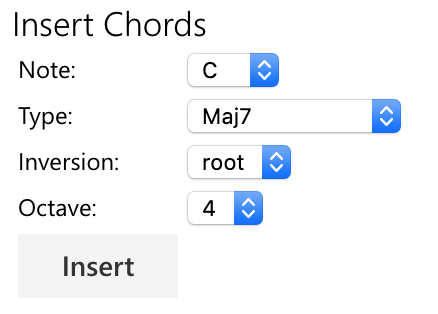
\includegraphics[width=50mm]{figs/insertChord.png}}
\caption{The interface within the add-in window for inserting the notes of chords.}
\label{fig:chordInput}
\end{figure}

\vspace{-20pt}
\paragraph{} The tonal \texttt{simplify} function reduces note definitions to contain at most one accidental, as required by Excello. This provides a list of notes in ascending order, without octaves or taking into account the inversion. To create the correct inversion of the chord, the array of notes is rotated by the inversion number.

\paragraph{} The given octave number is appended to the first note. A dictionary matches note names, accounting for enharmonics,\footnote{Notes that are the same pitch but different names, such as A$\flat$ and G$\sharp$.} to position in the chromatic scale starting at C (the first note of the octave in SPN). For each preceding note, if it appears in an equal or lower position in the scale than its predecessor, the octave number is incremented before appending. Otherwise, it is in the same octave, so the octave number is appended without modification.

\paragraph{} The selected range is acquired with the Office API. The chord notes are entered starting at the top-left corner of this range. If the range's height is greater or equal to its width, the notes are entered vertically going down. Otherwise, they are entered horizontally going right. Using the Office API, the range is set to the 2D array where the chord is entered.

\subsection{Custom Excel Functions}\label{Custom Excel Functions}

\paragraph{} Custom functions are implemented using another add-in. Rather than a separate window like the main Excello add-in, additional functions can be used in cells with the prefix ``\texttt{=EXCELLO.}". The file structure was generated with the Yeoman generator. The name, description, result type, and parameter names and types are stored in a JSON schema. This is used by Excel to provide argument prompts and autofill when writing formulae. Functions are defined in Typescript.

\paragraph{} The turtle function concatenates the arguments into the Excello turtle format. Other cells can be referenced, for example, the speed variable can reference a global tempo variable as in Figure \ref{implementation:turtleFunction}.

\paragraph{} The modulation function separates the note and volume for every note defined in a cell. The note is modulated using the tonal \texttt{Distance.transpose} function and recombined with the volume. The drag fill feature of Excel can be employed by the user to transpose sections or define melodic lines using the interval between notes as in Figure \ref{implementation:modulateFunction}.

\section{MIDI Converter}

\paragraph{} This section explains the Python converter from MIDI to CSV for Excello playback. A MIDI file is divided into up to 16 parallel tracks~\cite{midiSpec}. Each track contains a series of messages defined using predefined status and data bytes. I used the Mido library\footnote{https://mido.readthedocs.io/en/latest/index.html} to read MIDI files and abstract away from the underlying byte representations to view the messages. Note onsets and offsets are two separate events with two separate messages~\cite{midiSpec}. These messages include the note pitch, velocity, channel (not relevant) and time in ticks since the last message~\cite{midoSpec}.

\paragraph{} First, the list of messages is converted to a list of notes defined by onset and offset time, pitch and velocity. For each track, the messages are iterated through, using the time value in every message (including control and meta messages) to update a variable tracking time. For note onset messages, this is added to a dictionary mapping pitch to a list of currently active note start times. Lists are used because a pitch can be active multiple times at once. For note offset messages, or onset messages with zero velocity, the note popped from the active notes at that pitch with end time added is added to the list of all notes defined in the file.

\paragraph{} As each turtle only plays one note at a time, the notes are split into lists so no list contains concurrently played notes. Provided the initial list of notes is non-empty, a new list is created. The first remaining note is moved to the new list. Then iterating over the remaining notes, the next note starting after the previous note ends is moved to this new list. The number of iterations required is the number of turtles, $n$.

\paragraph{} If every tick corresponds to a cell, any combination of note onsets and offsets in a MIDI file can be accurately represented in Excello. To achieve smaller representations, the start and end times are converted to smaller cell numbers within the path of the turtle. For many MIDI files, the duration of a note is different from the time it occupies in notation. For example, a note immediately followed by another note in notation may have an end time significantly less than the start time of the next note in MIDI. A method is required to account for this. For all notes, before creating the different turtle streams, the length of the notes in ticks and differences between consecutive start times are found. The minimum value greater than 1 or modal value for these times are calculated depending on the compression level giving the $lengthStat$ and $di\hspace{-0.1em}f\hspace{-0.2em}f\hspace{-0.1em}erenceStat$.
\vspace{-10pt}

  $$ratio_{int} = \lfloor\max(lengthStat, di\hspace{-0.1em}f\hspace{-0.2em}f\hspace{-0.1em}erenceStat)/\min(lengthStat, di\hspace{-0.1em}f\hspace{-0.2em}f\hspace{-0.1em}erenceStat)\rfloor$$
  % $$ratio_{int} = \lfloor ratio \rfloor$$
  % $$correction = ratio/ratio_{int}$$
For each note, the times are adjusted as follows:
  $$length \gets (start - end) / lengthStat \text{ (rounded to the nearest 0.1)}$$
  $$start \gets start / di\hspace{-0.1em}f\hspace{-0.2em}f\hspace{-0.1em}erenceStat \times ratio_{int} \text{ (rounded to the nearest 0.1)}$$
  $$end \gets start +length$$

\paragraph{} The streams, with note start and end times corresponding to cells, are converted to a CSV file for Excello. Each turtle's path is initialised as an array of empty strings with length equal to the maximum end time for a note in any turtle, $L$. Each note the turtle plays is entered into the array. MIDI defines pitch using the integers. As there are 12 notes in an octave, modulus and division with 12 gives the note name and octave for SPN. If velocity is different from the previous note played by the turtle (or the note is the first note), the eight-bit MIDI velocity is mapped to Excello's [0,1] range. If the note length is greater than one, sustains are placed in the following cells. These paths go right starting in column A, with the first in row 2.

\paragraph{} Finally, the turtle definition is placed in the spreadsheet. The start cell range is ``A2:A$(n+1)$". The movement instruction is ``r m$L$". The MIDI file contains meta data for the \texttt{tempo} (milliseconds per beat) and \texttt{ticks\_per\_beat}. Cells per minute is calculated as follows:
$$cells\ per\ tick \times ticks\ per\ beat \times beat\ per\ minute$$
$$= \frac{ratio_{int}}{di\hspace{-0.1em}f\hspace{-0.2em}f\hspace{-0.1em}erenceStat} \times \texttt{ticks\_per\_beat} \times \frac{60 \times 10^6}{\texttt{tempo}}$$
With a value of 1 for repeats, the turtle definition is put in cell A1 and the CSV exported.

\newpage
\section{Repository Overview}

\tikzstyle{dir}=[draw=black,thick,anchor=west]
\tikzstyle{src}=[draw=black,thick,anchor=west,fill=red!30]
\tikzstyle{file}=[draw=black,thick,anchor=west,draw=none]

\begin{wrapfigure}{r}{8cm}
\vspace{-15pt}
% \begin{figure}[tbh]
\begin{tikzpicture}[%
  grow via three points={one child at (0.5,-0.7) and
  two children at (0.5,-0.7) and (0.5,-1.4)},
  edge from parent path={(\tikzparentnode.south) |- (\tikzchildnode.west)}]
  \node [dir] {Excello}
    child { node [dir] {Excel Music}
      child { node [dir] {assets}}
      child { node [dir] {node\_modules}}
      child { node [dir] {src}
        child { node [file] {index.ts}}
        child { node [file] {turtle.ts}}
        child { node [file] {chords.ts}}
        child { node [file] {regex.ts}}
        child { node [file] {conversions.ts}}
        child { node [file] {bracketsParse.ts}}
      }
      child [missing] {}
      child [missing] {}
      child [missing] {}
      child [missing] {}
      child [missing] {}
      child [missing] {}
      child { node [file] {index.html}}
      child { node [file] {manifest.xml}}
    }
    child [missing] {}
    child [missing] {}
    child [missing] {}
    child [missing] {}
    child [missing] {}
    child [missing] {}
    child [missing] {}
    child [missing] {}
    child [missing] {}
    child [missing] {}
    child [missing] {}
    child { node [dir] {CustomFunctions}
      child { node [dir] {src}
        child { node [file] {excello.ts}}
      }
      child [missing] {}
      child { node [dir] {config}
        child { node [file] {excello.json}}
      }
      child [missing] {}
      child { node [dir] {node\_modules}}
      child { node [file] {manifest.xml}}
    }
    child [missing] {}
    child [missing] {}
    child [missing] {}
    child [missing] {}
    child [missing] {}
    child [missing] {}
    child { node [dir] {MIDI}
      child { node [file] {MIDI\_Conversion.ipynb}}
    };
\end{tikzpicture}
\caption{File structure overview showing original files}
\label{fig:repo}
\vspace{-30pt}
% \end{figure}
\end{wrapfigure}

\paragraph{} Figure \ref{fig:repo} shows a reduced project file structure including all original source code. Excel Music is the add-in that parses the notation and produces music. Both this and CustomFunctions were generated using the Yeomann generator. The manifest.xml files are added to Excel and point to the resources to run the add-in. Users were given a different manifest pointing to a distribution hosted online with Surge. node\_modules contains all libraries required to run the add-ins and is managed using npm.

\paragraph{} The index.html file defines the window that appears on the right of the spreadsheet. assets contains the piano samples. index.ts defines what happens when the buttons of the window are pressed and imports from the remaining Typescript files. turtle.ts contains all the code to produce musical output from the spreadsheet, with helper functions in regex.ts, conversions.ts and bracketsParse.ts. bracketsParse.ts was based on Parenthesis which was initially incompatible for Excello's needs. chords.ts is for inserting chord notes into the grid.

\paragraph{} customFunctions.ts contains the implementation of EXCELLO.TURTLE and EXCELLO.MODULATE. The index.html file created when generating this add-in is not seen by the user so was not re-written.

\paragraph{} The Python notebook MIDI\_Conversion.ipynb converts MIDI files to the Excello notation. Conversions of MIDI corpora are included in the MIDI directory.

\paragraph{} I shall release Excello as an open source project under the MIT license. This is compatible with the MIT licenses of the libraries. The Salamander piano samples come under a creative commons license\footnote{https://creativecommons.org/licenses/by/3.0/.} so credit shall be given in the Excel add-in window.



%TC:group tabular 1 1
%TC:group table 1 1

\chapter{Implementation}

\paragraph{} This chapter shall explain how turtles are defined, and covers the remaining features of the initial prototype. The format and results of formative evaluation using this initial prototype shall be summarised, and the design decisions and changes that were made to Excello during the participatory design process will be discussed. Then, the technical details of Excello and the MIDI to Excello converter will be explained. It concludes with an overview of the project repository.

\section{Initial Prototype}

\begin{figure}[tbh]
\centerline{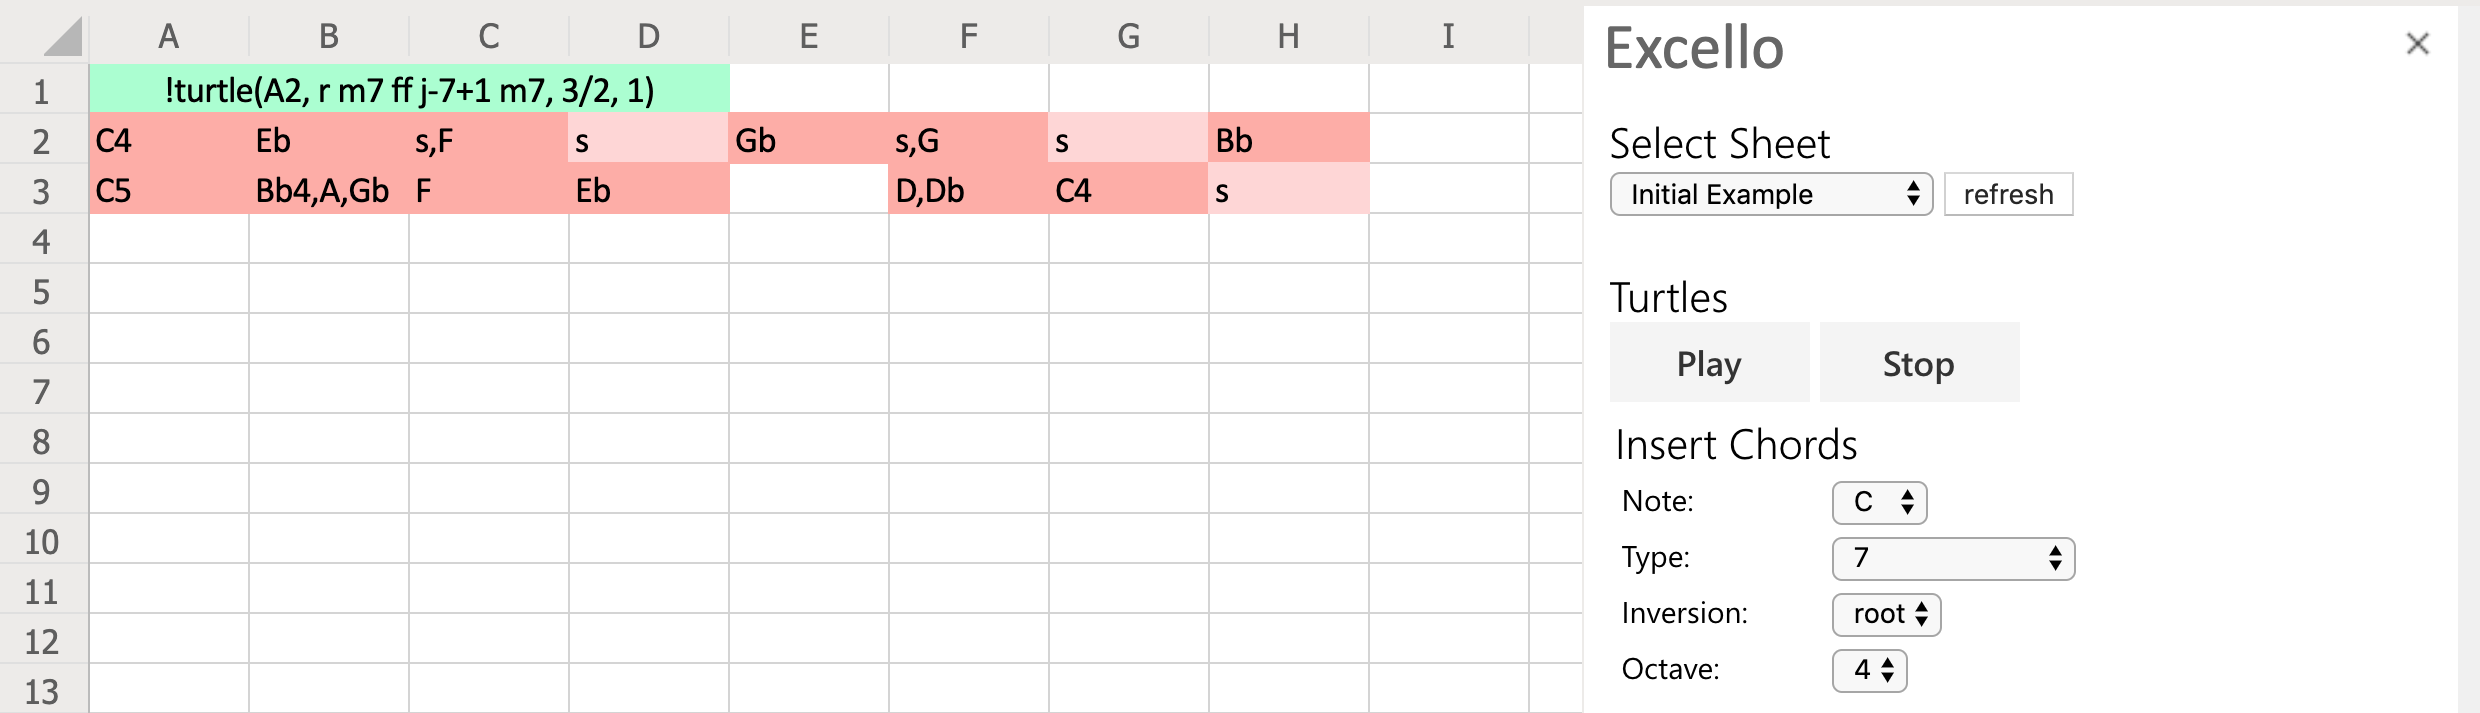
\includegraphics[width=150mm]{figs/initialPrototype.png}}
\caption{A two line motif defined in the initial Excello prototype}
\label{implementation:initialPrototype}
\end{figure}
\begin{figure}[tbh]
\centerline{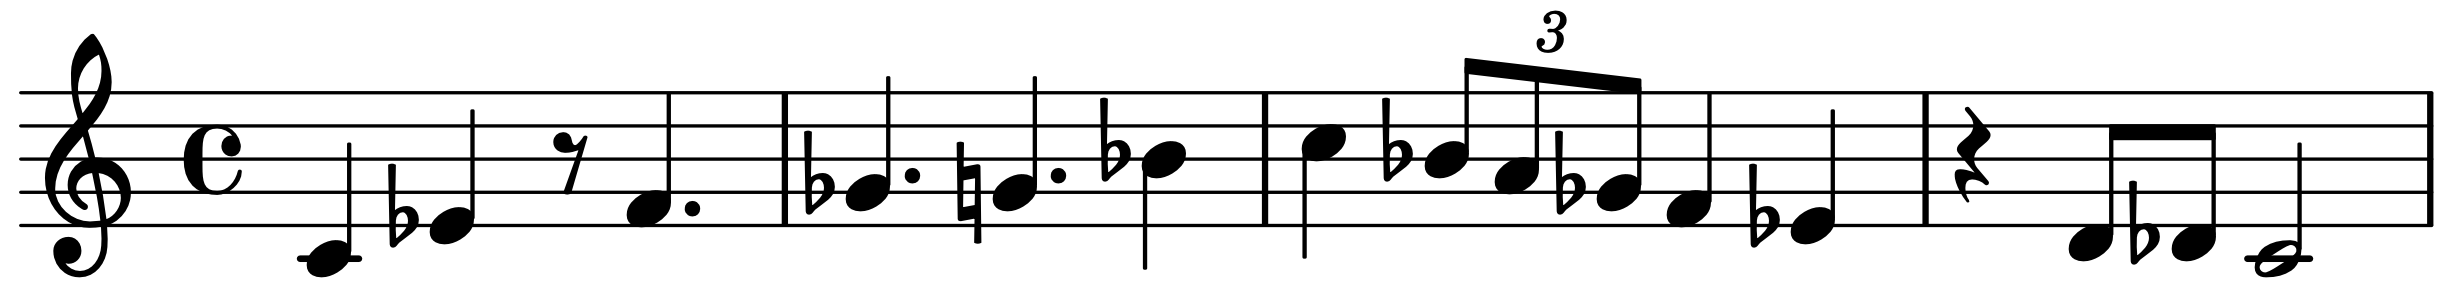
\includegraphics[width=150mm]{figs/initialScore.png}}
\caption{The notes played by the turtle in Figure \ref{implementation:initialPrototype}}
\label{implementation:initialScore}
\end{figure}

\vspace{-10pt}
\paragraph{} Notes and turtles can be defined in any cell. Turtles' interpretation of cells is shown in Table \ref{tab:cells}. When the Excello add-in is opened, a window opens on the right side of Excel as shown in Figure \ref{implementation:initialPrototype}. The melodic line produced is shown in figure \ref{implementation:initialScore}. Play and stop buttons launch all the turtles defined in the spreadsheet and initiate playback with a realistic piano sound.

\begin{table}[htb]
\centering
% \caption{Grammar Rules for the turtle movement instructions. $z \in \Z$}
\vspace{1pt}
\begin{tabular}{|l|l|} \hline
\textbf{Interpretation}&\textbf{Format}\\ \hline
Note& Name (A-G), optional accidental and octave number e.g.~\texttt{F$\sharp$4}\\ \hline
Sustain& \texttt{s}\\ \hline
Multiple notes& Notes, rests or sustains separated by a comma. Rests \\
subdivided in time& must be a space or an empty string e.g.~\texttt{E4,,C4,s}\\ \hline
Rest& Any cell not interpreted as a note, sustain or multi-note. \\ \hline
\end{tabular}
\caption{Interpretation of cells.\label{tab:cells}}
\end{table}

\subsection{Turtles}

\paragraph{} The following formula is enetered into a cell in the grid to define a turtle:\\
\texttt{!turtle(<Starting Cell>, <Movement>, <Speed>, <Number of Loops>)}

\vspace{-5pt}
\subsubsection{Activation}

\paragraph{} The prefix ``\texttt{!}" indicates the turtle will be activated when the play button is pressed. Just as digital audio workstations allow track muting and soloing, this can be used to modify which turtles play, without losing their definitions.

\vspace{-5pt}
\subsubsection{Starting Cell}

\paragraph{} The turtle's starting cell (\texttt{A2} in Figure \ref{implementation:initialPrototype}), which is also played, is a cell reference. As with Excel formulae, this is a concatenation of letters for the column and numbers for the row.

\paragraph{} As each turtle only plays one note at a time, multiple turtles must be defined to play polyphonic music such as chords. It was believed that users would define turtles following identical paths but in adjacent rows or columns. Multiple turtles following identical paths but starting from adjacent cells are defined using the existing Excel range notation for the starting cells. ``\texttt{A2:A5}" would define four turtles in the cells A2,A3,A4,A5. This prevents writing multiple turtle definitions differing in only the start cell row.

\vspace{-5pt}
\subsubsection{Movement}

\paragraph{} Turtles start facing north. The language for programming turtle movement is discussed in the Preparation chapter. The instructions are \texttt{r m7 ff j-7+1 m7} in Figure \ref{implementation:initialPrototype}. Using brackets to repeat movements had not been implemented by the start of the participatory design process.

\vspace{-5pt}
\subsubsection{Speed}

\paragraph{} An optional third argument is the speed of the turtle relative to 160 cells per minute. The default, 1, corresponds to 160 cells per minute. ``\texttt{3/2}", as in Figure \ref{implementation:initialPrototype}, would move the turtle at 240 cells per minute. Relative speed was used so it would be easier to tell the speed relation between turtles. This particularly suits phase music. Arbitrary maths can be provided, allowing turtles' speeds to be irrational multiples of each other.

\vspace{-5pt}
\subsubsection{Number of Loops}

\paragraph{} An optional fourth argument defines the number of repetitions of the turtle's entire path (\texttt{1} in Figure \ref{implementation:initialPrototype}). By default, the turtle loops infinitely. Repeating parts (e.g.~the cello in Pachelbel's Canon in D) therefore only need defining once.

\subsection{Highlighting}

\paragraph{} To assist recognising notes and turtles, when the play button is pressed, cells are highlighted. Activated or deactivated turtle definitions are highlighted green. Cells containing definitions of notes, or multiple notes, are highlighted red. Sustain cells are highlighted a lighter red, showing correspondence to notes whilst maintaining differentiation.

\subsection{Chord Input}

\paragraph{} To use the musical abstractions of chords whilst keeping the paradigm that a turtle is responsible for up to one note at any time, a tool to add chords is included. The note, type, inversion\footnote{Which note of the chord comes first, the other notes ascend from this. This is much like list rotations.} and starting octave of the chord are input into four drop-downs. The insert button enters the notes of the chord into the grid. If a single cell or a range taller than it is wide is highlighted in the spreadsheet, the notes are inserted vertically starting at the top-left of the range. Otherwise, the notes will be inserted horizontally. Whether the turtles are moving horizontally or vertically both chords and arpeggios\footnote{Where the notes of a chord are played individually in rising or descending order.} can be easily defined. Thus, helpful musical abstractions are still available whilst keeping the cleanness of the turtle system.

\section{Formative Evaluation}

\paragraph{} To guide development to best suit users, participants were involved in formative evaluation. Twenty-one University of Cambridge students, across a range of subjects, took part in the participatory design process. Initially, one-on-one tutorials on the initial prototype were given, followed by a short exercise. After these, users were interviewed on how they found Excello, drawing particular attention to actions that they found particularly unintuitive or requiring notable mental effort. Comparisons were made to musical interfaces with which participants were already familiar. The ethical and data handling procedures are discussed in the evaluation chapter.

\paragraph{} To realistically simulate how Excello would be used, participants carried out an exercise of their choice. Often this was transcribing a piece from memory or from traditional notation into the Excello notation. Two exercises were provided if participants had no immediate inspiration; transcribing a piece from western notation or changing existing Excello notation.

\paragraph{} These sessions were carried out in January 2019. Participants were asked to continue using Excello until the summative evaluation sessions in March. Additional feedback was collected as participants used Excello in their own time. This also ensured the summative evaluation was done with users that had sufficient experience of the interface.
% Participants were encouraged to get in contact with any additional issues or suggestions they had during this time.

\subsection{Issues and Suggestions}

\paragraph{} The issues and suggestions from the participatory design process are summarised below.

\subsubsection{Turtle Notation}

\paragraph{} Dynamics in the turtle instructions (e.g. \texttt{ppp m p m mf m ff m}) made establishing the turtle's path harder, as not all commands related to movement (``\texttt{m4}"). As the dynamics weren't next to the notes to which they corresponded, knowing the volume of a note or where to place the dynamics within the turtle to apply to notes in the spreadsheet was challenging. The initial prototype had no way to assign a dynamic to notes in the first cell. The starting cell could be empty, but this was inconvenient for looping parts, as this empty cell would be included in the loop. Users not familiar with western notation dynamics found them unintuitive. Furthermore, these discrete markings do not enable a continuous volume scale.

\paragraph{} When transcribing a piece, dividing its tempo by 160 for the relative speed caused unnecessary work. Users also forgot whether relative speed referred to the time spent in each cell or how quickly the turtle moved. Following the tutorial, users often had to check the position and meaning of turtle arguments.

\paragraph{} As the number of dynamics and movement commands grew, instructions became long and establishing turtle behaviour became cognitively challenging. Some users confused the ``\texttt{s}" within the turtle instructions to mean sustain (as it does in cells) and not south.

\subsubsection{Feedback}

\paragraph{} It was often unknown if pressing play actually registered, especially if the workbook saving delayed Excello's access to the spreadsheet. If a turtle had accidentally been left activated (with ``\texttt{!}"), the entire grid required searching to locate it. Users requested a summary of active turtle locations in addition to the highlighting.

\subsubsection{MIDI conversions}

\paragraph{} Users of production software said importing and exporting MIDI files would be helpful. If working with an existing MIDI file, converting that into the Excello notation would be convenient. Exportation would let Excello be used to create chord sequences, bass lines and the piece structure, before adding additional effects and recording in digital audio work stations.

\subsubsection{Sources of effort when writing}

\paragraph{} After inputting notes into the grid, the number of cells the turtle had to move required counting. As these were often in a straight line, the Excel status bar allowed users to select cells and immediately see how many there were. However, this was still not efficient, and was particularly inconvenient when users were writing notes and periodically testing what they had written so far. Some users instructed turtles to move forward significantly more steps than required to prevent counting. This is not feasible for looping parts. It was suggested that turtles could determine independently how far they should move.

\paragraph{} Instructions with repeated movements such as moving to the end of a line and jumping down to the beginning of a line below, required a lot of repetition.

\paragraph{} Many of the notes in melodic lines are frequently in the same octave. As such, repeatedly writing out the octave number was tiresome. One user made a comparison to LilyPond~\cite{sandberg:lily} where if the note length is not defined, the previous length would be used.

\paragraph{} Some users find it more intuitive to consider a melodic line by the intervals between notes rather than by the note names. A modulated\footnote{Where the pitch of every note in the sequence has moved by the same amount.} melody line required it to be written out again and could not be derived quicker any from the original version.

\subsubsection{Chords}

\paragraph{} Most users used a small subset of the available chord types, but had to find these within a large list. Separation of the more common chords was requested. Initially, notes inserted vertically had the lowest note at the top with pitch increasing down the column. Because higher pitch notes appear higher up the staff, it was suggested that inverting the order would be more intuitive. Initially, it was unclear what the different drop-downs corresponded to, with some users selecting the 7 from the octave number to try and insert a Maj7\footnote{A type of chord where the seventh note in the scale is added.} chord.

\subsubsection{Activation of Turtles}

\paragraph{} When toggling turtles' activations, entering the edit mode for each cell to add or remove the exclamation mark was very tedious.

\section{Second Prototype}

\paragraph{} Following the formative evaluation sessions and feedback, additions and modifications were made to solve the problems and opportunities that arose.

\subsection{Dynamics}

\paragraph{} To help extract a turtle's path and establish notes' volumes, dynamics are instead now inserted in the cells after the note, separated by a space as in Manhattan~\cite{nash:manhattan}. As before, this will apply to all following notes, until the volume is redefined. A single turtle definition with multiple start cells can now play parts of different volume. However, notes in the grid can be limited to only playing at their given volume. To play the same notes at a different volume, a new path must be made. Overall, the new system was believed to be preferable.

\paragraph{} To use a continuous volume scale, in addition to existing dynamic symbols, a number between 0 and 1 can instead be provided where 0 is silent and 1 is equivalent to \texttt{fff}.

\subsection{Nested Instructions}

\paragraph{} Nested instructions with repeats reduce turtle instructions and more easily incorporate repeated sections or movements. Multiple commands placed within parentheses followed by a number are repeated that number of times. Whilst the fourth argument of the turtle repeats the turtle's entire musical output, repetitions within the movement instructions allow paths to be defined more concisely.

\subsection{Absolute Tempo}

\paragraph{} The turtle's speed is now defined by cells per minute, rather than the relative value used initially. However, values less than 10 are interpreted in the original relative way for backwards compatibility with participants' existing work. To maintain consistency in a production version, this will be removed so speed must be defined absolutely. As speed and dynamics are different orders of magnitude, confusion between them is reduced.

\subsection{Custom Excel Functions}

\paragraph{} Two custom Excel functions have been implemented to aid composition. One to define turtles and a second to transpose notes. This allows Excello to take advantage of the functionality of the existing Excel ecosystem; drag-fill, autocomplete, cell referencing, etc.

\vspace{-20pt}
\texttt{\subsubsection{EXCELLO.TURTLE}}

\paragraph{} When writing a formula, a prompt informs users of the position of arguments, and whether they are optional. This outputs the turtle definition as text. All turtles could reference a single cell for their speeds. Relative tempi could then be implemented by the speed argument of each turtle being a multiple of this global speed as shown in Figure \ref{implementation:turtleFunction}.

\begin{figure}[tbh]
\centerline{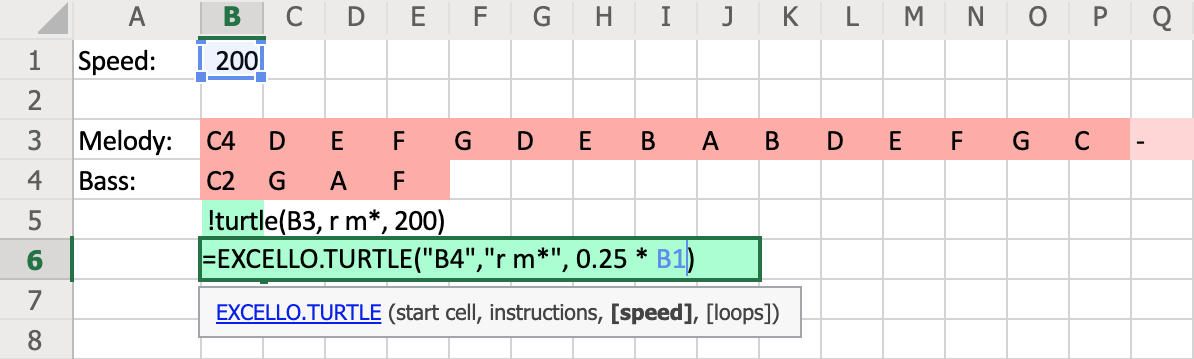
\includegraphics[width=150mm]{figs/turtleFunction.png}}
\caption{Defining a turtle using the \texttt{EXCELLO.TURTLE} function.}
\label{implementation:turtleFunction}
\end{figure}

\vspace{-30pt}
\texttt{\subsubsection{EXCELLO.MODULATE}}

\paragraph{} A modulating function lets melodic lines be defined by the intervals between notes and provides easy modulation of existing sections of a piece. The function takes a cell and an interval and outputs the cell with any notes transposed by the interval, maintaining any dynamics. A section can be modulated by calling this function on the first note with a provided interval and then using drag-fill. By using the previous note and one of a series of intervals as the arguments, a melodic line can quickly be produced from a starting note and a series of intervals as shown in Figure \ref{implementation:modulateFunction}.

\begin{figure}[tbh]
\centerline{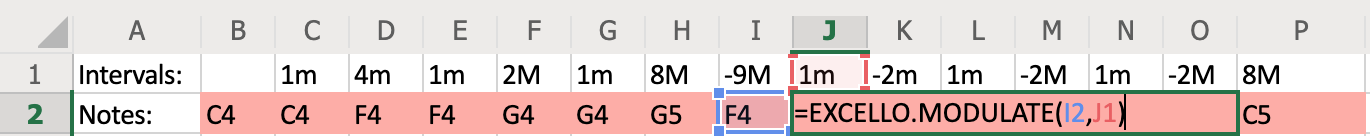
\includegraphics[width=150mm]{figs/modulateFunction.png}}
\caption{Transposing notes using the \texttt{EXCELLO.MODULATE} function.}
\label{implementation:modulateFunction}
\end{figure}

%  \ref{examples}

\subsection{Sustain}

\paragraph{} To prevent confusion between the south instruction and sustains. The symbol ``\texttt{-}" sustains a note. This was chosen because it is light and also has some similarity to a tie.\footnote{A line used in musical notation to increase the length of a note by joining it to another note.} Again, to maintain backwards compatibility, ``\texttt{s}" in a cell is still interpreted as a sustain.

\subsection{Active Turtles}

\paragraph{} To show that active turtle definitions have been recognised, a list of locations of the active turtles is given below the play button. This also helps find spurious turtles not intended to be activated.

\subsection{Automatic Movement}

\paragraph{} To prevent counting the cells in a line, \texttt{m*} instructs a turtle to move as far as there are notes or sustains defined in the direction it is facing. After adding more notes, the turtle instructions do not need editing before pressing play. A part may be meant to finish with a number of rests. As rests are notated with blank cells, a method to extend the path to include these rests was required. A cell can be explicitly defined as a rest with ``\texttt{.}". This is required if multiple turtles are playing a repeating section where one turtle's final cell as a note, sustain or multi-note cell. Without an explicit rest, the turtle would repeat too soon and the parts would consequently be out of phase.

\subsection{Inferred Octave}

\paragraph{} Octave numbers are inferred if omitted. Two methods were considered. Firstly, as most intervals within melodic lines are small, the nearest note could be played.
% This means that a scale would only need the octave defining in the first note.
Whilst this may require the fewest explicit statements of octave numbers, it would be hard to immediately identify the octave of any given note. The last defined octave in the path would need finding and then all subsequent notes walked through keeping track of the octave. The second consideration was to always use the last defined octave. Whilst this may require many octave definitions around the boundary between octaves, it is easier to find the octave of a note by backtracking. The second option was therefore implemented.

\subsection{Chords}

\paragraph{} To aid entering common chords, common types are repeated in a section at the top of the type drop-down. The chord drop-downs layout has been improved with labels to make it clearer what the values refer to. If the notes were entered vertically, the order was reversed, increasing correspondence with traditional staff notation.

\subsection{Activation of turtles}

\paragraph{} A ``Toggle Activation" button was added to the add-in window. When a cell or range is highlighted in the spreadsheet, the activation of any turtle definitions in this range will be toggled when the button is pressed.  This significantly decreases the time to toggle activations, as only two clicks are required, rather than entering the cell edit mode to add or remove an exclamation mark.

\section{Final Prototype Implementation}

\paragraph{} This section discusses the underlying implementation of the final prototype, following the participatory design. Excello consists of three main parts: the turtle system for playing the grid contents, the chord input tool, and the custom Excel functions.

\paragraph{} When the play button is pressed, turtle definitions in the grid are identified. For each, the starting cell and movement instructions are used to establish the contents of the cells it passes through. This is converted to a series of note definitions - pitch, start time, duration, volume. The speed and loop parameters are used to create the structure interpreted by the Tone.js library to schedule and initiate playback. An overview of the data flow and subtasks required to create the musical playback is shown in Figure \ref{fig:overview}.

\begin{figure}[htb]
\begin{center}
  
  \tikzset{every picture/.style={line width=0.75pt}} %set default line width to 0.75pt

  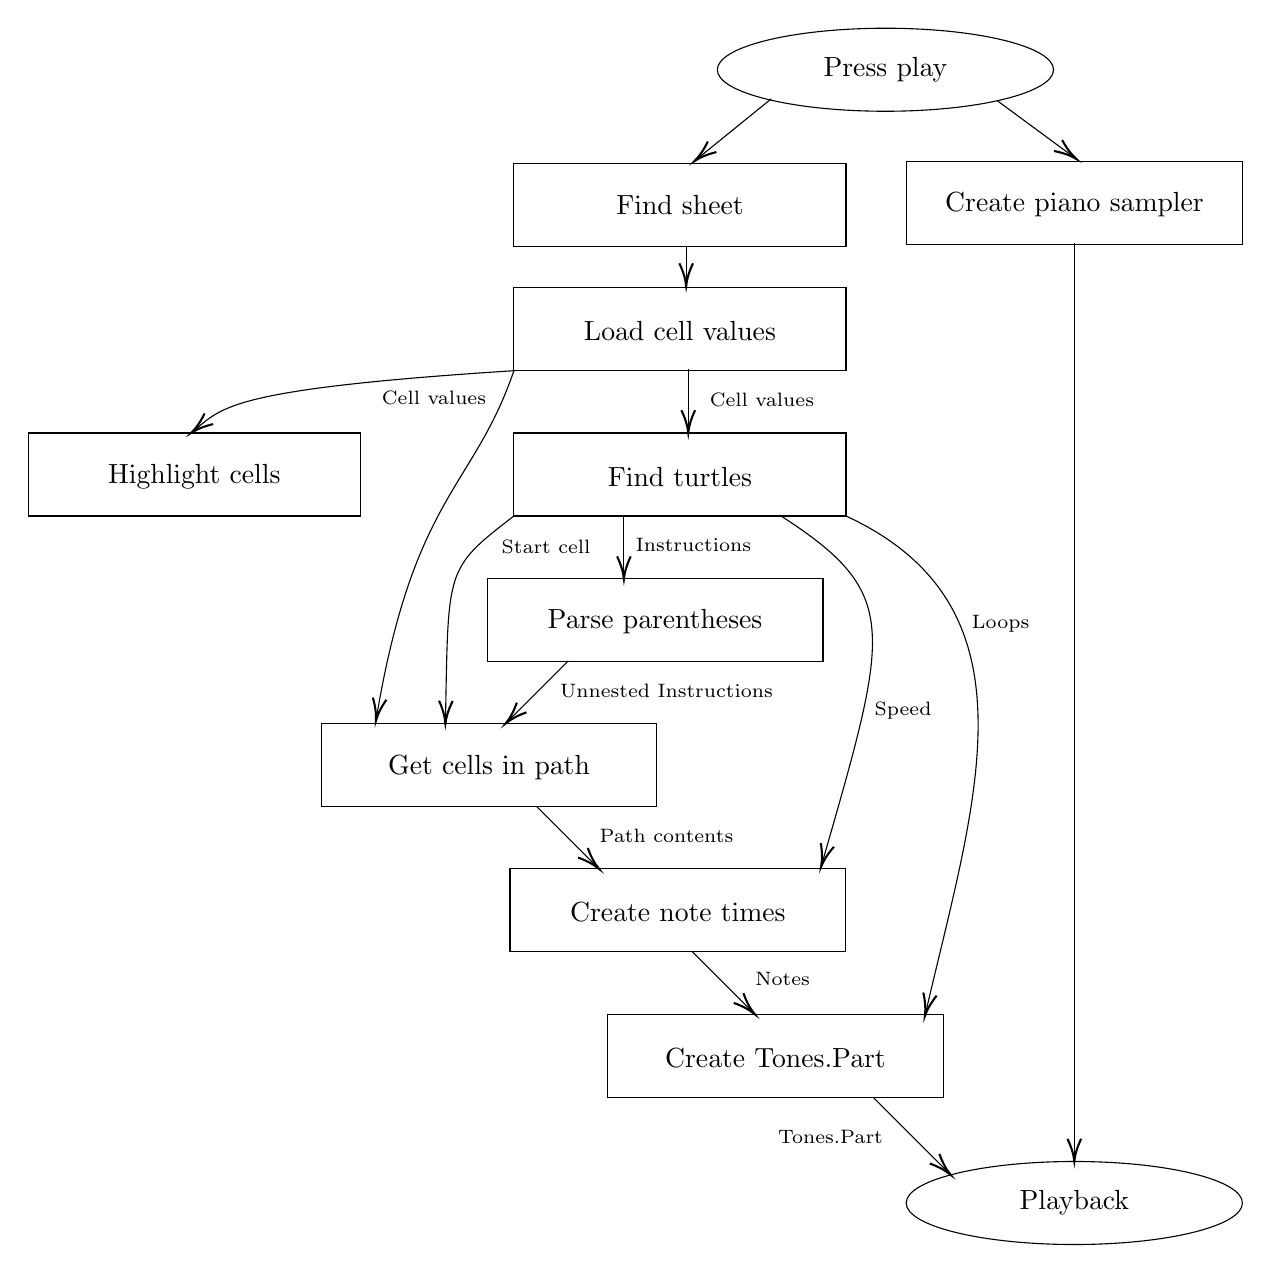
\begin{tikzpicture}[x=0.75pt,y=0.75pt,yscale=-1,xscale=1]
  %uncomment if require: \path (0,604); %set diagram left start at 0, and has height of 604

  %Shape: Rectangle [id:dp3390223975782729]
  \draw   (244.5,71) -- (404.5,71) -- (404.5,111) -- (244.5,111) -- cycle ;

  %Shape: Rectangle [id:dp7168559924493858]
  \draw   (244.5,131) -- (404.5,131) -- (404.5,171) -- (244.5,171) -- cycle ;

  %Shape: Rectangle [id:dp8835932361497658]
  \draw   (433.7,70) -- (595.5,70) -- (595.5,110) -- (433.7,110) -- cycle ;

  %Shape: Rectangle [id:dp9464422191216635]
  \draw   (244.5,201) -- (404.5,201) -- (404.5,241) -- (244.5,241) -- cycle ;

  %Shape: Rectangle [id:dp6384624480751633]
  \draw   (231.6,271) -- (393.4,271) -- (393.4,311) -- (231.6,311) -- cycle ;

  %Shape: Rectangle [id:dp2927464084046889]
  \draw   (151.6,341) -- (313.4,341) -- (313.4,381) -- (151.6,381) -- cycle ;

  %Shape: Rectangle [id:dp9052659554068596]
  \draw   (242.6,411) -- (404.4,411) -- (404.4,451) -- (242.6,451) -- cycle ;

  %Shape: Rectangle [id:dp5637329489183025]
  \draw   (289.6,481) -- (451.4,481) -- (451.4,521) -- (289.6,521) -- cycle ;

  %Curve Lines [id:da3917180624639185]
  \draw    (244.5,241) .. controls (211.17,266.67) and (212.98,265.81) .. (211.52,339.88) ;
  \draw [shift={(211.5,341)}, rotate = 271.14] [color={rgb, 255:red, 0; green, 0; blue, 0 }  ][line width=0.75]    (10.93,-3.29) .. controls (6.95,-1.4) and (3.31,-0.3) .. (0,0) .. controls (3.31,0.3) and (6.95,1.4) .. (10.93,3.29)   ;

  %Straight Lines [id:da6961662223442007]
  \draw    (297.5,241) -- (297.5,269.4) ;
  \draw [shift={(297.5,271.4)}, rotate = 270] [color={rgb, 255:red, 0; green, 0; blue, 0 }  ][line width=0.75]    (10.93,-3.29) .. controls (6.95,-1.4) and (3.31,-0.3) .. (0,0) .. controls (3.31,0.3) and (6.95,1.4) .. (10.93,3.29)   ;

  %Curve Lines [id:da9168950950169605]
  \draw    (372.6,240.6) .. controls (431.31,278.41) and (425.56,294.84) .. (392.99,408.28) ;
  \draw [shift={(392.5,410)}, rotate = 286.01] [color={rgb, 255:red, 0; green, 0; blue, 0 }  ][line width=0.75]    (10.93,-3.29) .. controls (6.95,-1.4) and (3.31,-0.3) .. (0,0) .. controls (3.31,0.3) and (6.95,1.4) .. (10.93,3.29)   ;

  %Curve Lines [id:da7972588626438504]
  \draw    (404.5,241) .. controls (499.03,284.78) and (466.83,377.07) .. (442.86,480.44) ;
  \draw [shift={(442.5,482)}, rotate = 282.99] [color={rgb, 255:red, 0; green, 0; blue, 0 }  ][line width=0.75]    (10.93,-3.29) .. controls (6.95,-1.4) and (3.31,-0.3) .. (0,0) .. controls (3.31,0.3) and (6.95,1.4) .. (10.93,3.29)   ;

  %Straight Lines [id:da6822022155717844]
  \draw    (270.7,310.8) -- (241.91,339.59) ;
  \draw [shift={(240.5,341)}, rotate = 315] [color={rgb, 255:red, 0; green, 0; blue, 0 }  ][line width=0.75]    (10.93,-3.29) .. controls (6.95,-1.4) and (3.31,-0.3) .. (0,0) .. controls (3.31,0.3) and (6.95,1.4) .. (10.93,3.29)   ;

  %Straight Lines [id:da4884596231580207]
  \draw    (255.5,381) -- (284.09,409.59) ;
  \draw [shift={(285.5,411)}, rotate = 225] [color={rgb, 255:red, 0; green, 0; blue, 0 }  ][line width=0.75]    (10.93,-3.29) .. controls (6.95,-1.4) and (3.31,-0.3) .. (0,0) .. controls (3.31,0.3) and (6.95,1.4) .. (10.93,3.29)   ;

  %Straight Lines [id:da9233366942734922]
  \draw    (330.5,451) -- (359.09,479.59) ;
  \draw [shift={(360.5,481)}, rotate = 225] [color={rgb, 255:red, 0; green, 0; blue, 0 }  ][line width=0.75]    (10.93,-3.29) .. controls (6.95,-1.4) and (3.31,-0.3) .. (0,0) .. controls (3.31,0.3) and (6.95,1.4) .. (10.93,3.29)   ;

  %Straight Lines [id:da3670498457872964]
  \draw    (417.5,521) -- (453.49,556.99) ;
  \draw [shift={(454.9,558.4)}, rotate = 225] [color={rgb, 255:red, 0; green, 0; blue, 0 }  ][line width=0.75]    (10.93,-3.29) .. controls (6.95,-1.4) and (3.31,-0.3) .. (0,0) .. controls (3.31,0.3) and (6.95,1.4) .. (10.93,3.29)   ;

  %Straight Lines [id:da28794703530347365]
  \draw    (327.5,111) -- (327.5,128.2) ;
  \draw [shift={(327.5,130.2)}, rotate = 270] [color={rgb, 255:red, 0; green, 0; blue, 0 }  ][line width=0.75]    (10.93,-3.29) .. controls (6.95,-1.4) and (3.31,-0.3) .. (0,0) .. controls (3.31,0.3) and (6.95,1.4) .. (10.93,3.29)   ;

  %Straight Lines [id:da33376731250782754]
  \draw    (328.5,170) -- (328.5,199) ;
  \draw [shift={(328.5,201)}, rotate = 270] [color={rgb, 255:red, 0; green, 0; blue, 0 }  ][line width=0.75]    (10.93,-3.29) .. controls (6.95,-1.4) and (3.31,-0.3) .. (0,0) .. controls (3.31,0.3) and (6.95,1.4) .. (10.93,3.29)   ;

  %Curve Lines [id:da2676626927985757]
  \draw    (244.5,171) .. controls (225.1,227.72) and (196.29,230.77) .. (178.27,338.17) ;
  \draw [shift={(178,339.8)}, rotate = 279.38] [color={rgb, 255:red, 0; green, 0; blue, 0 }  ][line width=0.75]    (10.93,-3.29) .. controls (6.95,-1.4) and (3.31,-0.3) .. (0,0) .. controls (3.31,0.3) and (6.95,1.4) .. (10.93,3.29)   ;

  %Straight Lines [id:da024649031996502035]
  \draw    (514.5,109.6) -- (514.5,550) ;
  \draw [shift={(514.5,552)}, rotate = 270] [color={rgb, 255:red, 0; green, 0; blue, 0 }  ][line width=0.75]    (10.93,-3.29) .. controls (6.95,-1.4) and (3.31,-0.3) .. (0,0) .. controls (3.31,0.3) and (6.95,1.4) .. (10.93,3.29)   ;

  %Shape: Ellipse [id:dp13505581605963868]
  \draw   (433.5,572) .. controls (433.5,560.95) and (469.76,552) .. (514.5,552) .. controls (559.24,552) and (595.5,560.95) .. (595.5,572) .. controls (595.5,583.05) and (559.24,592) .. (514.5,592) .. controls (469.76,592) and (433.5,583.05) .. (433.5,572) -- cycle ;

  %Shape: Ellipse [id:dp006287630832967794]
  \draw   (342.5,26) .. controls (342.5,14.95) and (378.76,6) .. (423.5,6) .. controls (468.24,6) and (504.5,14.95) .. (504.5,26) .. controls (504.5,37.05) and (468.24,46) .. (423.5,46) .. controls (378.76,46) and (342.5,37.05) .. (342.5,26) -- cycle ;

  %Straight Lines [id:da09048722077694915]
  \draw    (368.5,40) -- (333.05,68.74) ;
  \draw [shift={(331.5,70)}, rotate = 320.96000000000004] [color={rgb, 255:red, 0; green, 0; blue, 0 }  ][line width=0.75]    (10.93,-3.29) .. controls (6.95,-1.4) and (3.31,-0.3) .. (0,0) .. controls (3.31,0.3) and (6.95,1.4) .. (10.93,3.29)   ;

  %Straight Lines [id:da9578993167654264]
  \draw    (477.5,41) -- (513.89,67.81) ;
  \draw [shift={(515.5,69)}, rotate = 216.38] [color={rgb, 255:red, 0; green, 0; blue, 0 }  ][line width=0.75]    (10.93,-3.29) .. controls (6.95,-1.4) and (3.31,-0.3) .. (0,0) .. controls (3.31,0.3) and (6.95,1.4) .. (10.93,3.29)   ;

  %Shape: Rectangle [id:dp25073410390478523]
  \draw   (10.5,201) -- (170.5,201) -- (170.5,241) -- (10.5,241) -- cycle ;

  %Curve Lines [id:da2454539812308738]
  \draw    (244.5,171) .. controls (108.92,179.69) and (104.17,188.37) .. (90.53,199.75) ;
  \draw [shift={(89,201)}, rotate = 321.34000000000003] [color={rgb, 255:red, 0; green, 0; blue, 0 }  ][line width=0.75]    (10.93,-3.29) .. controls (6.95,-1.4) and (3.31,-0.3) .. (0,0) .. controls (3.31,0.3) and (6.95,1.4) .. (10.93,3.29)   ;


  % Text Node
  \draw (324.5,91) node  [align=left] {Find sheet};
  % Text Node
  \draw (324.5,152) node  [align=left] {Load cell values};
  % Text Node
  \draw (514.6,91) node  [align=left] {Create piano sampler};
  % Text Node
  \draw (324.5,222) node  [align=left] {Find turtles};
  % Text Node
  \draw (312.5,292) node  [align=left] {Parse parentheses};
  % Text Node
  \draw (232.5,362) node  [align=left] {Get cells in path};
  % Text Node
  \draw (323.5,432) node  [align=left] {Create note times};
  % Text Node
  \draw (370.5,502) node  [align=left] {Create Tones.Part};
  % Text Node
  \draw (514.5,572) node [] [align=left] {\textcolor[rgb]{0,0,0}{Playback}};
  % Text Node
  \draw (260,256) node  [align=left] {{\scriptsize Start cell}};
  % Text Node
  \draw (331,255) node  [align=left] {{\scriptsize Instructions}};
  % Text Node
  \draw (432,335) node  [align=left] {{\scriptsize Speed}};
  % Text Node
  \draw (479,293) node  [align=left] {{\scriptsize Loops}};
  % Text Node
  \draw (318,325) node  [align=left] {{\scriptsize Unnested Instructions}};
  % Text Node
  \draw (318,395) node  [align=left] {{\scriptsize Path contents}};
  % Text Node
  \draw (374,464) node  [align=left] {{\scriptsize Notes}};
  % Text Node
  \draw (397,540) node  [align=left] {{\scriptsize Tones.Part}};
  % Text Node
  \draw (206,184) node  [align=left] {{\scriptsize Cell values}};
  % Text Node
  \draw (423.5,26) node [] [align=left] {Press play};
  % Text Node
  \draw (364,185) node  [align=left] {{\scriptsize Cell values}};
  % Text Node
  \draw (90.5,222) node  [align=left] {Highlight cells};


  \end{tikzpicture}

\end{center}
\caption{An overview of the playback algorithm and dataflow of Excello\label{fig:overview}}
\end{figure}

\paragraph{} The \texttt{Sampler} is an extension of the \texttt{Tone.Instrument} class. This interpolates between pitched samples to create arbitrary notes. A sampler is loaded using the Salamander grand piano samples~\footnote{https://freepats.zenvoid.org/Piano/acoustic-grand-piano.html} which includes four pitches (out of a possible 12) per octave. This accurately interpolates notes whilst reducing loading times and storage requirements.

\subsection{Identifying Cells}

\paragraph{} A drop-down is populated with names loaded using the Office API. Having pressed play, the cell values from the selected sheet are loaded and then analysed for highlighting and calculating the musical output. Cells containing at least one note definition are highlighted red. A note must contain a note name, optional accidental, optional octave number, and optional volume instruction following a space. This is a dynamic marking or number between 0 and 1. Notes are identified using the following regular expression:

\begin{verbatim}
^[A-G](#|b|)?[1-9]?( (0(\.\[0-9]+)?|1(\.0)?|ppp|pp|p|mp|mf|f|ff|fff))?$
\end{verbatim}

\paragraph{} Cells containing multiple definitions (e.g. ``\texttt{C4 ff,-, ,D}", ``\texttt{,,G,F$\sharp$}") are split using commas. The resulting strings are trimmed of starting and ending whitespace and then must either be a note, sustain (``\texttt{-}" or ``\texttt{s}"), explicit rest (``\texttt{.}") or empty string (created from trimming a rest). Cells matching ``\texttt{-}",``\texttt{.}" or ``\texttt{s}" are highlighted a lighter red. Turtle definitions (e.g. ``\texttt{!turtle(B2:B4, r m*, 200, 1)}") are identified using:
\begin{verbatim}
^(!turtle\().*(\))$
\end{verbatim}
and these cells are highlighted green. The addresses of cells containing a turtle definition are added to the live turtle section of the add-in window.

\subsection{Parsing Movement Instructions}

\paragraph{} Movement instructions are converted to a single unnested list of commands (e.g.~``\texttt{(r m2)2}" becomes ``\texttt{[r, m2, r, m2]}") so the turtle's path can be established. The \texttt{parse} method of the Parenthesis\footnote{https://www.npmjs.com/package/parenthesis} library seemed suitable for aiding this string manipulation. This parses strings containing brackets into a nested array. For example, \texttt{parse(\textcolor[rgb]{0,0.7,0}{\upquote{a(b[c\{d\}])}})} gives \texttt{[\textcolor[rgb]{0,0.7,0}{\upquote{a(}}, [\textcolor[rgb]{0,0.7,0}{\upquote{b[}}, [\textcolor[rgb]{0,0.7,0}{\upquote{c\{}}, [\textcolor[rgb]{0,0.7,0}{\upquote{d}}], \textcolor[rgb]{0,0.7,0}{\upquote{\}}}], \textcolor[rgb]{0,0.7,0}{\upquote{]}}], \textcolor[rgb]{0,0.7,0}{\upquote{)}}]}.

\paragraph{} This suggests the string ``\texttt{(r m2)2}" would become \texttt{[\upquote{(}, [\upquote{r m2}], \upquote{)2}]}. By removing the brackets from these strings, a simple recursive method could be built to output \texttt{\upquote{r m2 r m2}} from \texttt{[[\upquote{r m2}], \upquote{2}]}. However, upon testing this, the library outputted an undefined array. From investigating the source code, I established that strings with a number following a closing parenthesis all produced this error. Substituting characters for the numbers or placing a symbol before all numbers and then later removing these would allow the library to be used. Instead, using the Parenthesis method as inspiration, I implemented my own parsing function tailored to Excello.

\paragraph{} This has two main steps. First, the deepest bracketed expression is stored in an array with the brackets removed. This expression is replaced in the original string with the string \upquote{\texttt{\_\_\_}$x$\texttt{\_\_\_}} where $x$ is the expression's index in the array. This is repeated until the string contains no brackets. Then a recursive function uses the values of $x$ to reconstruct the string in the nested array format. This method is outlined in Algorithm \ref{alg:parenthesis}. The Typescript implementation is in Appendix \ref{appendix:parseBrackets}.

\begin{algorithm}[!htp]
\caption{Parsing bracketed expression. \texttt{str.replace(regex,f)} (line 13) performs \texttt{f(s)} on the first substring, \texttt{s}, of \texttt{str} matching the regular expression \texttt{regex}.}
\label{alg:parenthesis}
\begin{algorithmic}[1]
\Procedure{parseBrackets}{$str$}

   \State $idPadding\gets \texttt{\upquote{\_\_\_}}$
   \State $unnestedStr\gets []$
   \State $deepestLevelBracketsRE\gets \texttt{RegExp(\upquote{\textbackslash\textbackslash([\^{}\textbackslash\textbackslash(\textbackslash\textbackslash)]*\textbackslash\textbackslash)})}$
   \State $replacementIDRE\gets \texttt{RegExp(\upquote{\textbackslash\textbackslash} + }idPadding\texttt{ + \upquote{([0-9]+)} + }idPadding\texttt{)}$\\

   \Procedure{replaceDeepestBracket}{$x$}
     \State \texttt{unnestedStr.push(x.substring(1, x.length-1))}
     \State \texttt{\textbf{return} idPadding + (unnestedStr.length - 1) + idPadding}
   \EndProcedure \\

   \While{\texttt{deepestLevelBracketsRE.test(str)}}
     \State \texttt{str = str.replace(deepestLevelBracketsRE,replaceDeepestBracket)}
   \EndWhile

   \State \texttt{unnestedStr[0] = str}\\

   \Procedure{reNest}{$outerStr$}
     \State $renestingStr\gets []$
     \While{There is a match of $replacementIDRE$ in $outerStr$}
       \State $matchIndex\gets$ index of the match in $outerStr$
       \State $matchID\gets$ ID of the match (number between padding)
       \State $matchString\gets$ matched string\\

       \If{$matchIndex >$ 0}
				\State $renestingStr$.push($outestStr$.substring(0, $matchIndex$))
			\EndIf
			\State $renestingStr$.push(reNest($unnestedStr$[$firstMatchID$]))
			\State $outestStr$ = $outestStr$.substring($matchIndex$ + $matchString$.length)
     \EndWhile
     \State $renestingStr$.push($outestStr$)
     \State \textbf{return} $renestingStr$
   \EndProcedure \\

   \State \textbf{return} \textsc{reNest}($unnestedStr$[0])

\EndProcedure
\end{algorithmic}
\end{algorithm}


\paragraph{} Having submitted a bug report on the Parenthesis GitHub, and implemented my own method for parsing turtle movement instructions, I implemented a fix to the Parenthesis library. The library previously performed replacements with the string \upquote{\texttt{\_\_\_}$x$}. $x$ and following numbers would concatenate forming a single number, causing the library to fail. My method of having an identifier before and after $x$ fixed this issue. I also added additional tests to Parenthesis to verify my method and ensure that previous tests all passed before submitting a pull request. I have made an open source contribution, as this has since been merged into the library and published.

\paragraph{} I wrote an additional recursive method to unnest the array into a single stream of commands. An empty string, \texttt{s}, is initialised. For each item in the array, if it is an array, unnest the contents recursively and add the result to s. If not, it will be one or more single movement commands. If the single movement commands start with a number, the result is added to \texttt{s} that number of times. The remaining instructions are added to \texttt{s}. This is outlined in Algorithm \ref{alg:unnest}. The implementation is shown in Appendix \ref{appendix:processParsedBrackets}.

\begin{algorithm}[!htbp]
\caption{Unnesting parsed bracketed expressions.}
\label{alg:unnest}
\begin{algorithmic}[1]
\Procedure{processParsedBrackets}{$arr$}

   \State $s\gets \texttt{\upquote{}}$
   \State $previousArr$

   \For{$v$ in $s$}
    \If{$v$ is an array}
     \State $previousArr \gets$ processParsedBrackets($v$)
    \Else
       \If{previous instruction was an array}
        \State $s \gets s + previousArr$
        \If{next instruction is a number}
          \State $s \gets s + previousArr$, that number of times minus one
        \EndIf
       \EndIf
       \State $s \gets s + $ remaining instruction in $v$
    \EndIf
   \EndFor
   \State \textbf{return} $s$

\EndProcedure
\end{algorithmic}
\end{algorithm}

\subsection{Getting Cells in Turtles' Paths}

\paragraph{} If the turtle's first argument defines a range of starting cells, the cell addresses of this range are calculated. For each starting cell, the unnested instructions and sheet values are used to find the contents of the cells the turtle passes through. This process models the movement of the turtle within the grid, keeping track of its position and the direction in which it is facing. For each instruction, the position and direction are updated as required, and the contents of any new cells entered are added to a list of notes.

\paragraph{} For the ``\texttt{m*}" instruction, the number of steps the turtle takes must be computed. Given the turtle's current position and direction, the one-dimensional array of cells in front of it is taken. The turtle should step to the last cell that defines a note, sustain or explicit rest. The number of steps is the array's length minus the index of the first element in the reversed array satisfying this criterion.

\subsection{Creating Note Times}

\paragraph{} The cells a turtle moves through are used to create a data structure containing the information for playback using the Tone library. For each turtle, the following array is produced: \texttt{[[<Note 1>,...,<Note N>], <number of cells>]} (note sequence array). Each note is as follows: \texttt{[<start time>, [<pitch>, <duration>, <volume>]]}. Volume and octave are added to each note if they were omitted from a cell.

\paragraph{} The Tone Transport is a timeline along which events can be scheduled. This supports many different representations of time. I used Transport Time for all note onsets and durations. This is of the form \texttt{\upquote{BARS:QUARTERS:SIXTEENTHS}} where the three values are numbers and can be non-integer. With \texttt{QUARTERS} representing the number of cells, the calculation of exact times, or arbitrary musical notes can be avoided. This allows the contents of cells to be easily converted to times to be interpreted by the Tones library.

\paragraph{} The note sequence array is initiated by counting the notes that are defined in the cell contents using regular expressions for identifying notes and multi-note cells. The cells are iterated through keeping track of the active note and adding it to the note sequence when it ends. Outside of this loop, variables track how many cells and notes through the process the algorithm is and whether it is currently a rest or note. Variables keep track of the note currently being played - when it started (\texttt{currentStart}), the pitch (\texttt{currentNote}) and the volume (\texttt{currentVolume}). As volume and octave number may be omitted, variables also keep track of these. Table \ref{tab:times} outlines the actions performed when a cell is read. Notes are added to the note sequence in the form \texttt{[currentStart, [currentNote, \upquote{0:} + noteLength + \upquote{:0}, currentVolume]]}.

\begin{table}[ht]
\begin{tabular}{|l|l|l|l|l|}
  \hline
  \textbf{Cell}&\textbf{State}&\multicolumn{3}{c|}{\textbf{Action}} \\
  \hline
  \multirow{5}{*}{Note}&\multirow{3}{*}{Note}&Note, octave and &Previous note added&currentStart = \\
  &&volume established&to note sequence&\upquote{0:}+beatCount+\upquote{:0}\\
  &&from cell contents&&currentNote = value\\
  \cline{2-2}
  \cline{4-4}
  &\multirow{2}{*}{Rest}&and previous values&inRest = false&noteLength = 1\\
  &&&&currentVolume = volume\\
  \hline
  \multirow{2}{*}{Sustain}&Note&\multicolumn{3}{l|}{noteLength++}\\
  \cline{2-5}
  &Rest&\multicolumn{3}{l|}{Nothing (has no semantic value)}\\
  \hline
  \multirow{3}{*}{Rest}&\multirow{2}{*}{Note}&\multicolumn{3}{l|}{Previous note added to note sequence}\\
  &&\multicolumn{3}{l|}{inRest = true}\\
  \cline{2-5}
  &Rest&\multicolumn{3}{l|}{Nothing}\\
  \hline
\end{tabular}
\caption{The actions taken when processing each cell to create note times. The beat count corresponds to the cell number being processed and is incremented each time.\label{tab:times}}
\end{table}
\vspace{-10pt}

\paragraph{} The same method is used for multi-note cells, except the note length and cell count are incremented by the appropriate fraction for each item in the cell. If, after the final cell, the state is a note, it is ended and added to the note sequence.

\paragraph{} The values in the note sequence are sufficient for the piano sampler to play a note using the \texttt{triggerAttackRelease} function. The \texttt{Tone.Part} class allows multiple calls to this method to be defined, started, stopped and looped as a single unit. This is defined with the note sequence and its speed set with the evaluated turtle speed argument. The number of cells, calculated when creating the note times, number of repeats, and the evaluated speed argument are used to control when looping ends.

% \begin{verbatim}
% var turtlePart = new Tone.Part(function(time, note){
%   piano.triggerAttackRelease(note[0], note[1], time, note[2]);
% }, noteTimes).start();
% if (repeats>0){
%   turtlePart = turtlePart.stop("0:" + (repeats*beatsLength/speedFactor) + ":0");
% }
% turtlePart.loop = true;
% turtlePart.loopEnd = "0:" + beatsLength + ":0";
% turtlePart.playbackRate = speedFactor;
% \end{verbatim}

% \begin{lstlisting}[style=js]
%   var turtlePart = new Tone.Part(function(time, note){
%     piano.triggerAttackRelease(note[0], note[1], time, note[2]);
%   }, noteTimes).start();
%   if (repeats>0){
%     turtlePart = turtlePart.stop("0:" + (repeats*beatsLength/speedFactor) + ":0");
%   }
%   turtlePart.loop = true;
%   turtlePart.loopEnd = "0:" + beatsLength + ":0";
%   turtlePart.playbackRate = speedFactor;
% \end{lstlisting}

\subsection{Chord Input}\label{Chord Input}

\paragraph{} The next two subsections (\S\ref{Chord Input} and \S\ref{Custom Excel Functions}) outline the two smaller parts of the Excello; the chord input tool, and the custom Excel functions. When the insert button in the add-in window is pressed, the note, type, inversion and octave of the chord are extracted from their HTML elements. The chord interface within the add-in window is shown in Figure \ref{fig:chordInput}. The tonal library is used to generate the chord notes:

\begin{verbatim}
var chordNotes = Chord.notes(chordNote, chordType).map(x => Note.simplify(x));
\end{verbatim}
\vspace{-10pt}

\begin{figure}[htb]
\centerline{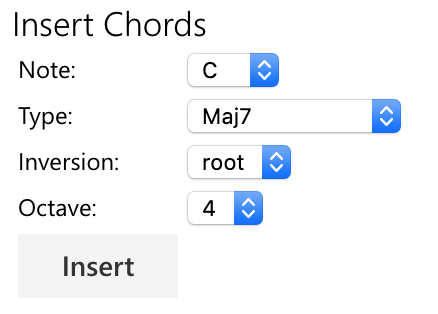
\includegraphics[width=50mm]{figs/insertChord.png}}
\caption{The interface within the add-in window for inserting the notes of chords.}
\label{fig:chordInput}
\end{figure}

\vspace{-20pt}
\paragraph{} The tonal \texttt{simplify} function reduces note definitions to contain at most one accidental, as required by Excello. This provides a list of notes in ascending order, without octaves or taking into account the inversion. To create the correct inversion of the chord, the array of notes is rotated by the inversion number.

\paragraph{} The given octave number is appended to the first note. A dictionary matches note names, accounting for enharmonics,\footnote{Notes that are the same pitch but different names, such as A$\flat$ and G$\sharp$.} to position in the chromatic scale starting at C (the first note of the octave in SPN). For each preceding note, if it appears in an equal or lower position in the scale than its predecessor, the octave number is incremented before appending. Otherwise, it is in the same octave, so the octave number is appended without modification.

\paragraph{} The selected range is acquired with the Office API. The chord notes are entered starting at the top-left corner of this range. If the range's height is greater or equal to its width, the notes are entered vertically going down. Otherwise, they are entered horizontally going right. Using the Office API, the range is set to the 2D array where the chord is entered.

\subsection{Custom Excel Functions}\label{Custom Excel Functions}

\paragraph{} Custom functions are implemented using another add-in. Rather than a separate window like the main Excello add-in, additional functions can be used in cells with the prefix ``\texttt{=EXCELLO.}". The file structure was generated with the Yeoman generator. The name, description, result type, and parameter names and types are stored in a JSON schema. This is used by Excel to provide argument prompts and autofill when writing formulae. Functions are defined in Typescript.

\paragraph{} The turtle function concatenates the arguments into the Excello turtle format. Other cells can be referenced, for example, the speed variable can reference a global tempo variable as in Figure \ref{implementation:turtleFunction}.

\paragraph{} The modulation function separates the note and volume for every note defined in a cell. The note is modulated using the tonal \texttt{Distance.transpose} function and recombined with the volume. The drag fill feature of Excel can be employed by the user to transpose sections or define melodic lines using the interval between notes as in Figure \ref{implementation:modulateFunction}.

\section{MIDI Converter}

\paragraph{} This section explains the Python converter from MIDI to CSV for Excello playback. A MIDI file is divided into up to 16 parallel tracks~\cite{midiSpec}. Each track contains a series of messages defined using predefined status and data bytes. I used the Mido library\footnote{https://mido.readthedocs.io/en/latest/index.html} to read MIDI files and abstract away from the underlying byte representations to view the messages. Note onsets and offsets are two separate events with two separate messages~\cite{midiSpec}. These messages include the note pitch, velocity, channel (not relevant) and time in ticks since the last message~\cite{midoSpec}.

\paragraph{} First, the list of messages is converted to a list of notes defined by onset and offset time, pitch and velocity. For each track, the messages are iterated through, using the time value in every message (including control and meta messages) to update a variable tracking time. For note onset messages, this is added to a dictionary mapping pitch to a list of currently active note start times. Lists are used because a pitch can be active multiple times at once. For note offset messages, or onset messages with zero velocity, the note popped from the active notes at that pitch with end time added is added to the list of all notes defined in the file.

\paragraph{} As each turtle only plays one note at a time, the notes are split into lists so no list contains concurrently played notes. Provided the initial list of notes is non-empty, a new list is created. The first remaining note is moved to the new list. Then iterating over the remaining notes, the next note starting after the previous note ends is moved to this new list. The number of iterations required is the number of turtles, $n$.

\paragraph{} If every tick corresponds to a cell, any combination of note onsets and offsets in a MIDI file can be accurately represented in Excello. To achieve smaller representations, the start and end times are converted to smaller cell numbers within the path of the turtle. For many MIDI files, the duration of a note is different from the time it occupies in notation. For example, a note immediately followed by another note in notation may have an end time significantly less than the start time of the next note in MIDI. A method is required to account for this. For all notes, before creating the different turtle streams, the length of the notes in ticks and differences between consecutive start times are found. The minimum value greater than 1 or modal value for these times are calculated depending on the compression level giving the $lengthStat$ and $di\hspace{-0.1em}f\hspace{-0.2em}f\hspace{-0.1em}erenceStat$.
\vspace{-10pt}

  $$ratio_{int} = \lfloor\max(lengthStat, di\hspace{-0.1em}f\hspace{-0.2em}f\hspace{-0.1em}erenceStat)/\min(lengthStat, di\hspace{-0.1em}f\hspace{-0.2em}f\hspace{-0.1em}erenceStat)\rfloor$$
  % $$ratio_{int} = \lfloor ratio \rfloor$$
  % $$correction = ratio/ratio_{int}$$
For each note, the times are adjusted as follows:
  $$length \gets (start - end) / lengthStat \text{ (rounded to the nearest 0.1)}$$
  $$start \gets start / di\hspace{-0.1em}f\hspace{-0.2em}f\hspace{-0.1em}erenceStat \times ratio_{int} \text{ (rounded to the nearest 0.1)}$$
  $$end \gets start +length$$

\paragraph{} The streams, with note start and end times corresponding to cells, are converted to a CSV file for Excello. Each turtle's path is initialised as an array of empty strings with length equal to the maximum end time for a note in any turtle, $L$. Each note the turtle plays is entered into the array. MIDI defines pitch using the integers. As there are 12 notes in an octave, modulus and division with 12 gives the note name and octave for SPN. If velocity is different from the previous note played by the turtle (or the note is the first note), the eight-bit MIDI velocity is mapped to Excello's [0,1] range. If the note length is greater than one, sustains are placed in the following cells. These paths go right starting in column A, with the first in row 2.

\paragraph{} Finally, the turtle definition is placed in the spreadsheet. The start cell range is ``A2:A$(n+1)$". The movement instruction is ``r m$L$". The MIDI file contains meta data for the \texttt{tempo} (milliseconds per beat) and \texttt{ticks\_per\_beat}. Cells per minute is calculated as follows:
$$cells\ per\ tick \times ticks\ per\ beat \times beat\ per\ minute$$
$$= \frac{ratio_{int}}{di\hspace{-0.1em}f\hspace{-0.2em}f\hspace{-0.1em}erenceStat} \times \texttt{ticks\_per\_beat} \times \frac{60 \times 10^6}{\texttt{tempo}}$$
With a value of 1 for repeats, the turtle definition is put in cell A1 and the CSV exported.

\newpage
\section{Repository Overview}

\tikzstyle{dir}=[draw=black,thick,anchor=west]
\tikzstyle{src}=[draw=black,thick,anchor=west,fill=red!30]
\tikzstyle{file}=[draw=black,thick,anchor=west,draw=none]

\begin{wrapfigure}{r}{8cm}
\vspace{-15pt}
% \begin{figure}[tbh]
\begin{tikzpicture}[%
  grow via three points={one child at (0.5,-0.7) and
  two children at (0.5,-0.7) and (0.5,-1.4)},
  edge from parent path={(\tikzparentnode.south) |- (\tikzchildnode.west)}]
  \node [dir] {Excello}
    child { node [dir] {Excel Music}
      child { node [dir] {assets}}
      child { node [dir] {node\_modules}}
      child { node [dir] {src}
        child { node [file] {index.ts}}
        child { node [file] {turtle.ts}}
        child { node [file] {chords.ts}}
        child { node [file] {regex.ts}}
        child { node [file] {conversions.ts}}
        child { node [file] {bracketsParse.ts}}
      }
      child [missing] {}
      child [missing] {}
      child [missing] {}
      child [missing] {}
      child [missing] {}
      child [missing] {}
      child { node [file] {index.html}}
      child { node [file] {manifest.xml}}
    }
    child [missing] {}
    child [missing] {}
    child [missing] {}
    child [missing] {}
    child [missing] {}
    child [missing] {}
    child [missing] {}
    child [missing] {}
    child [missing] {}
    child [missing] {}
    child [missing] {}
    child { node [dir] {CustomFunctions}
      child { node [dir] {src}
        child { node [file] {excello.ts}}
      }
      child [missing] {}
      child { node [dir] {config}
        child { node [file] {excello.json}}
      }
      child [missing] {}
      child { node [dir] {node\_modules}}
      child { node [file] {manifest.xml}}
    }
    child [missing] {}
    child [missing] {}
    child [missing] {}
    child [missing] {}
    child [missing] {}
    child [missing] {}
    child { node [dir] {MIDI}
      child { node [file] {MIDI\_Conversion.ipynb}}
    };
\end{tikzpicture}
\caption{File structure overview showing original files}
\label{fig:repo}
\vspace{-30pt}
% \end{figure}
\end{wrapfigure}

\paragraph{} Figure \ref{fig:repo} shows a reduced project file structure including all original source code. Excel Music is the add-in that parses the notation and produces music. Both this and CustomFunctions were generated using the Yeomann generator. The manifest.xml files are added to Excel and point to the resources to run the add-in. Users were given a different manifest pointing to a distribution hosted online with Surge. node\_modules contains all libraries required to run the add-ins and is managed using npm.

\paragraph{} The index.html file defines the window that appears on the right of the spreadsheet. assets contains the piano samples. index.ts defines what happens when the buttons of the window are pressed and imports from the remaining Typescript files. turtle.ts contains all the code to produce musical output from the spreadsheet, with helper functions in regex.ts, conversions.ts and bracketsParse.ts. bracketsParse.ts was based on Parenthesis which was initially incompatible for Excello's needs. chords.ts is for inserting chord notes into the grid.

\paragraph{} customFunctions.ts contains the implementation of EXCELLO.TURTLE and EXCELLO.MODULATE. The index.html file created when generating this add-in is not seen by the user so was not re-written.

\paragraph{} The Python notebook MIDI\_Conversion.ipynb converts MIDI files to the Excello notation. Conversions of MIDI corpora are included in the MIDI directory.

\paragraph{} I shall release Excello as an open source project under the MIT license. This is compatible with the MIT licenses of the libraries. The Salamander piano samples come under a creative commons license\footnote{https://creativecommons.org/licenses/by/3.0/.} so credit shall be given in the Excel add-in window.



%TC:group tabular 1 1
%TC:group table 1 1

\chapter{Implementation}

\paragraph{} This chapter shall explain how turtles are defined, and covers the remaining features of the initial prototype. The format and results of formative evaluation using this initial prototype shall be summarised, and the design decisions and changes that were made to Excello during the participatory design process will be discussed. Then, the technical details of Excello and the MIDI to Excello converter will be explained. It concludes with an overview of the project repository.

\section{Initial Prototype}

\begin{figure}[tbh]
\centerline{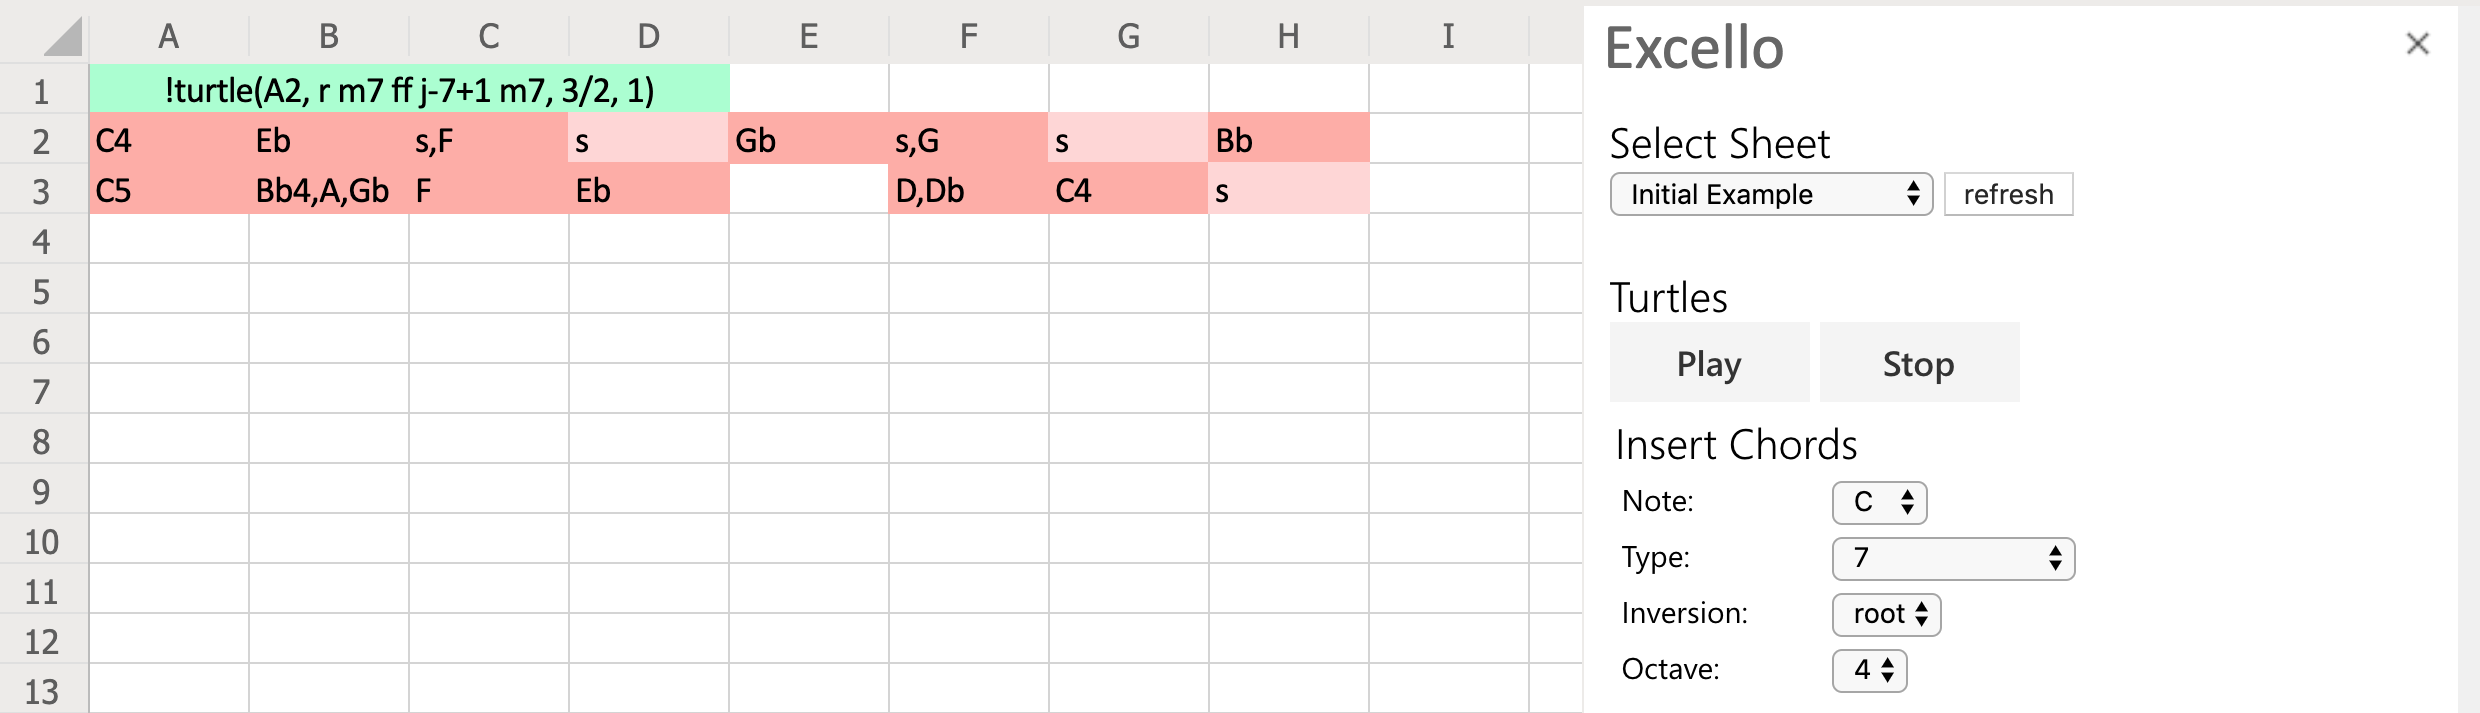
\includegraphics[width=150mm]{figs/initialPrototype.png}}
\caption{A two line motif defined in the initial Excello prototype}
\label{implementation:initialPrototype}
\end{figure}
\begin{figure}[tbh]
\centerline{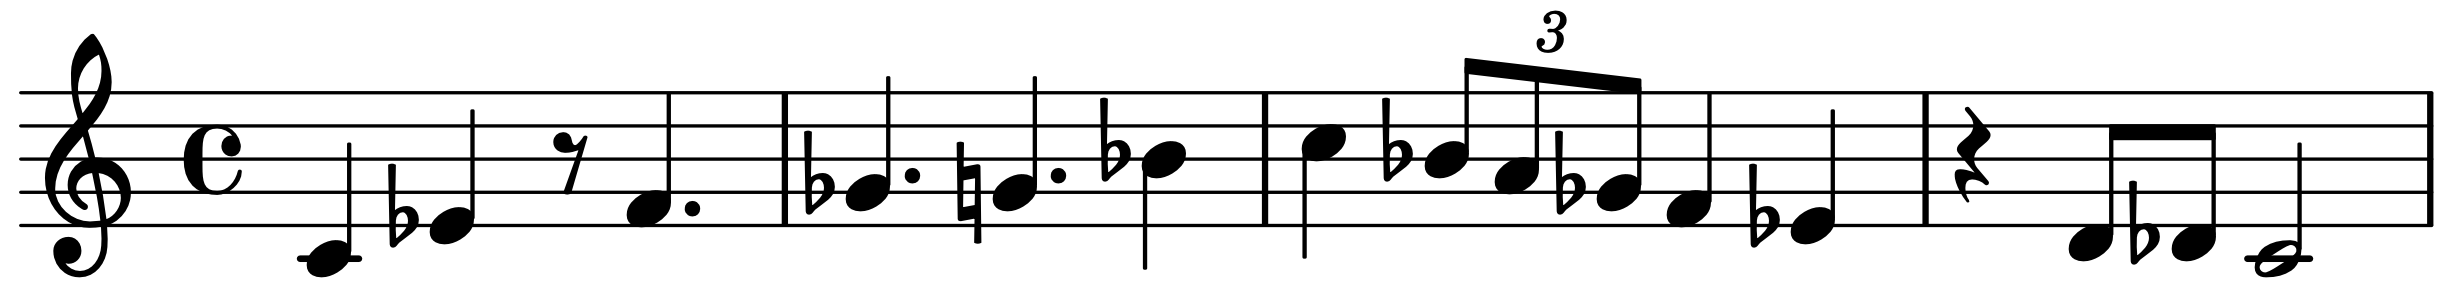
\includegraphics[width=150mm]{figs/initialScore.png}}
\caption{The notes played by the turtle in Figure \ref{implementation:initialPrototype}}
\label{implementation:initialScore}
\end{figure}

\vspace{-10pt}
\paragraph{} Notes and turtles can be defined in any cell. Turtles' interpretation of cells is shown in Table \ref{tab:cells}. When the Excello add-in is opened, a window opens on the right side of Excel as shown in Figure \ref{implementation:initialPrototype}. The melodic line produced is shown in figure \ref{implementation:initialScore}. Play and stop buttons launch all the turtles defined in the spreadsheet and initiate playback with a realistic piano sound.

\begin{table}[htb]
\centering
% \caption{Grammar Rules for the turtle movement instructions. $z \in \Z$}
\vspace{1pt}
\begin{tabular}{|l|l|} \hline
\textbf{Interpretation}&\textbf{Format}\\ \hline
Note& Name (A-G), optional accidental and octave number e.g.~\texttt{F$\sharp$4}\\ \hline
Sustain& \texttt{s}\\ \hline
Multiple notes& Notes, rests or sustains separated by a comma. Rests \\
subdivided in time& must be a space or an empty string e.g.~\texttt{E4,,C4,s}\\ \hline
Rest& Any cell not interpreted as a note, sustain or multi-note. \\ \hline
\end{tabular}
\caption{Interpretation of cells.\label{tab:cells}}
\end{table}

\subsection{Turtles}

\paragraph{} The following formula is enetered into a cell in the grid to define a turtle:\\
\texttt{!turtle(<Starting Cell>, <Movement>, <Speed>, <Number of Loops>)}

\vspace{-5pt}
\subsubsection{Activation}

\paragraph{} The prefix ``\texttt{!}" indicates the turtle will be activated when the play button is pressed. Just as digital audio workstations allow track muting and soloing, this can be used to modify which turtles play, without losing their definitions.

\vspace{-5pt}
\subsubsection{Starting Cell}

\paragraph{} The turtle's starting cell (\texttt{A2} in Figure \ref{implementation:initialPrototype}), which is also played, is a cell reference. As with Excel formulae, this is a concatenation of letters for the column and numbers for the row.

\paragraph{} As each turtle only plays one note at a time, multiple turtles must be defined to play polyphonic music such as chords. It was believed that users would define turtles following identical paths but in adjacent rows or columns. Multiple turtles following identical paths but starting from adjacent cells are defined using the existing Excel range notation for the starting cells. ``\texttt{A2:A5}" would define four turtles in the cells A2,A3,A4,A5. This prevents writing multiple turtle definitions differing in only the start cell row.

\vspace{-5pt}
\subsubsection{Movement}

\paragraph{} Turtles start facing north. The language for programming turtle movement is discussed in the Preparation chapter. The instructions are \texttt{r m7 ff j-7+1 m7} in Figure \ref{implementation:initialPrototype}. Using brackets to repeat movements had not been implemented by the start of the participatory design process.

\vspace{-5pt}
\subsubsection{Speed}

\paragraph{} An optional third argument is the speed of the turtle relative to 160 cells per minute. The default, 1, corresponds to 160 cells per minute. ``\texttt{3/2}", as in Figure \ref{implementation:initialPrototype}, would move the turtle at 240 cells per minute. Relative speed was used so it would be easier to tell the speed relation between turtles. This particularly suits phase music. Arbitrary maths can be provided, allowing turtles' speeds to be irrational multiples of each other.

\vspace{-5pt}
\subsubsection{Number of Loops}

\paragraph{} An optional fourth argument defines the number of repetitions of the turtle's entire path (\texttt{1} in Figure \ref{implementation:initialPrototype}). By default, the turtle loops infinitely. Repeating parts (e.g.~the cello in Pachelbel's Canon in D) therefore only need defining once.

\subsection{Highlighting}

\paragraph{} To assist recognising notes and turtles, when the play button is pressed, cells are highlighted. Activated or deactivated turtle definitions are highlighted green. Cells containing definitions of notes, or multiple notes, are highlighted red. Sustain cells are highlighted a lighter red, showing correspondence to notes whilst maintaining differentiation.

\subsection{Chord Input}

\paragraph{} To use the musical abstractions of chords whilst keeping the paradigm that a turtle is responsible for up to one note at any time, a tool to add chords is included. The note, type, inversion\footnote{Which note of the chord comes first, the other notes ascend from this. This is much like list rotations.} and starting octave of the chord are input into four drop-downs. The insert button enters the notes of the chord into the grid. If a single cell or a range taller than it is wide is highlighted in the spreadsheet, the notes are inserted vertically starting at the top-left of the range. Otherwise, the notes will be inserted horizontally. Whether the turtles are moving horizontally or vertically both chords and arpeggios\footnote{Where the notes of a chord are played individually in rising or descending order.} can be easily defined. Thus, helpful musical abstractions are still available whilst keeping the cleanness of the turtle system.

\section{Formative Evaluation}

\paragraph{} To guide development to best suit users, participants were involved in formative evaluation. Twenty-one University of Cambridge students, across a range of subjects, took part in the participatory design process. Initially, one-on-one tutorials on the initial prototype were given, followed by a short exercise. After these, users were interviewed on how they found Excello, drawing particular attention to actions that they found particularly unintuitive or requiring notable mental effort. Comparisons were made to musical interfaces with which participants were already familiar. The ethical and data handling procedures are discussed in the evaluation chapter.

\paragraph{} To realistically simulate how Excello would be used, participants carried out an exercise of their choice. Often this was transcribing a piece from memory or from traditional notation into the Excello notation. Two exercises were provided if participants had no immediate inspiration; transcribing a piece from western notation or changing existing Excello notation.

\paragraph{} These sessions were carried out in January 2019. Participants were asked to continue using Excello until the summative evaluation sessions in March. Additional feedback was collected as participants used Excello in their own time. This also ensured the summative evaluation was done with users that had sufficient experience of the interface.
% Participants were encouraged to get in contact with any additional issues or suggestions they had during this time.

\subsection{Issues and Suggestions}

\paragraph{} The issues and suggestions from the participatory design process are summarised below.

\subsubsection{Turtle Notation}

\paragraph{} Dynamics in the turtle instructions (e.g. \texttt{ppp m p m mf m ff m}) made establishing the turtle's path harder, as not all commands related to movement (``\texttt{m4}"). As the dynamics weren't next to the notes to which they corresponded, knowing the volume of a note or where to place the dynamics within the turtle to apply to notes in the spreadsheet was challenging. The initial prototype had no way to assign a dynamic to notes in the first cell. The starting cell could be empty, but this was inconvenient for looping parts, as this empty cell would be included in the loop. Users not familiar with western notation dynamics found them unintuitive. Furthermore, these discrete markings do not enable a continuous volume scale.

\paragraph{} When transcribing a piece, dividing its tempo by 160 for the relative speed caused unnecessary work. Users also forgot whether relative speed referred to the time spent in each cell or how quickly the turtle moved. Following the tutorial, users often had to check the position and meaning of turtle arguments.

\paragraph{} As the number of dynamics and movement commands grew, instructions became long and establishing turtle behaviour became cognitively challenging. Some users confused the ``\texttt{s}" within the turtle instructions to mean sustain (as it does in cells) and not south.

\subsubsection{Feedback}

\paragraph{} It was often unknown if pressing play actually registered, especially if the workbook saving delayed Excello's access to the spreadsheet. If a turtle had accidentally been left activated (with ``\texttt{!}"), the entire grid required searching to locate it. Users requested a summary of active turtle locations in addition to the highlighting.

\subsubsection{MIDI conversions}

\paragraph{} Users of production software said importing and exporting MIDI files would be helpful. If working with an existing MIDI file, converting that into the Excello notation would be convenient. Exportation would let Excello be used to create chord sequences, bass lines and the piece structure, before adding additional effects and recording in digital audio work stations.

\subsubsection{Sources of effort when writing}

\paragraph{} After inputting notes into the grid, the number of cells the turtle had to move required counting. As these were often in a straight line, the Excel status bar allowed users to select cells and immediately see how many there were. However, this was still not efficient, and was particularly inconvenient when users were writing notes and periodically testing what they had written so far. Some users instructed turtles to move forward significantly more steps than required to prevent counting. This is not feasible for looping parts. It was suggested that turtles could determine independently how far they should move.

\paragraph{} Instructions with repeated movements such as moving to the end of a line and jumping down to the beginning of a line below, required a lot of repetition.

\paragraph{} Many of the notes in melodic lines are frequently in the same octave. As such, repeatedly writing out the octave number was tiresome. One user made a comparison to LilyPond~\cite{sandberg:lily} where if the note length is not defined, the previous length would be used.

\paragraph{} Some users find it more intuitive to consider a melodic line by the intervals between notes rather than by the note names. A modulated\footnote{Where the pitch of every note in the sequence has moved by the same amount.} melody line required it to be written out again and could not be derived quicker any from the original version.

\subsubsection{Chords}

\paragraph{} Most users used a small subset of the available chord types, but had to find these within a large list. Separation of the more common chords was requested. Initially, notes inserted vertically had the lowest note at the top with pitch increasing down the column. Because higher pitch notes appear higher up the staff, it was suggested that inverting the order would be more intuitive. Initially, it was unclear what the different drop-downs corresponded to, with some users selecting the 7 from the octave number to try and insert a Maj7\footnote{A type of chord where the seventh note in the scale is added.} chord.

\subsubsection{Activation of Turtles}

\paragraph{} When toggling turtles' activations, entering the edit mode for each cell to add or remove the exclamation mark was very tedious.

\section{Second Prototype}

\paragraph{} Following the formative evaluation sessions and feedback, additions and modifications were made to solve the problems and opportunities that arose.

\subsection{Dynamics}

\paragraph{} To help extract a turtle's path and establish notes' volumes, dynamics are instead now inserted in the cells after the note, separated by a space as in Manhattan~\cite{nash:manhattan}. As before, this will apply to all following notes, until the volume is redefined. A single turtle definition with multiple start cells can now play parts of different volume. However, notes in the grid can be limited to only playing at their given volume. To play the same notes at a different volume, a new path must be made. Overall, the new system was believed to be preferable.

\paragraph{} To use a continuous volume scale, in addition to existing dynamic symbols, a number between 0 and 1 can instead be provided where 0 is silent and 1 is equivalent to \texttt{fff}.

\subsection{Nested Instructions}

\paragraph{} Nested instructions with repeats reduce turtle instructions and more easily incorporate repeated sections or movements. Multiple commands placed within parentheses followed by a number are repeated that number of times. Whilst the fourth argument of the turtle repeats the turtle's entire musical output, repetitions within the movement instructions allow paths to be defined more concisely.

\subsection{Absolute Tempo}

\paragraph{} The turtle's speed is now defined by cells per minute, rather than the relative value used initially. However, values less than 10 are interpreted in the original relative way for backwards compatibility with participants' existing work. To maintain consistency in a production version, this will be removed so speed must be defined absolutely. As speed and dynamics are different orders of magnitude, confusion between them is reduced.

\subsection{Custom Excel Functions}

\paragraph{} Two custom Excel functions have been implemented to aid composition. One to define turtles and a second to transpose notes. This allows Excello to take advantage of the functionality of the existing Excel ecosystem; drag-fill, autocomplete, cell referencing, etc.

\vspace{-20pt}
\texttt{\subsubsection{EXCELLO.TURTLE}}

\paragraph{} When writing a formula, a prompt informs users of the position of arguments, and whether they are optional. This outputs the turtle definition as text. All turtles could reference a single cell for their speeds. Relative tempi could then be implemented by the speed argument of each turtle being a multiple of this global speed as shown in Figure \ref{implementation:turtleFunction}.

\begin{figure}[tbh]
\centerline{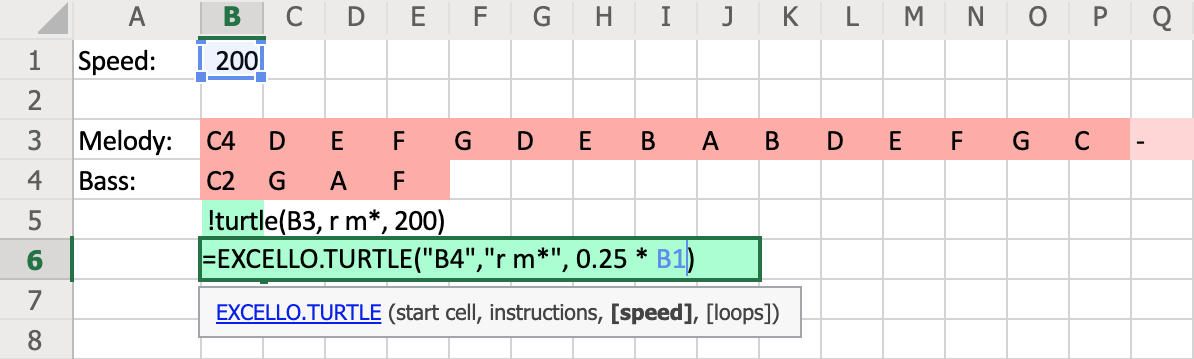
\includegraphics[width=150mm]{figs/turtleFunction.png}}
\caption{Defining a turtle using the \texttt{EXCELLO.TURTLE} function.}
\label{implementation:turtleFunction}
\end{figure}

\vspace{-30pt}
\texttt{\subsubsection{EXCELLO.MODULATE}}

\paragraph{} A modulating function lets melodic lines be defined by the intervals between notes and provides easy modulation of existing sections of a piece. The function takes a cell and an interval and outputs the cell with any notes transposed by the interval, maintaining any dynamics. A section can be modulated by calling this function on the first note with a provided interval and then using drag-fill. By using the previous note and one of a series of intervals as the arguments, a melodic line can quickly be produced from a starting note and a series of intervals as shown in Figure \ref{implementation:modulateFunction}.

\begin{figure}[tbh]
\centerline{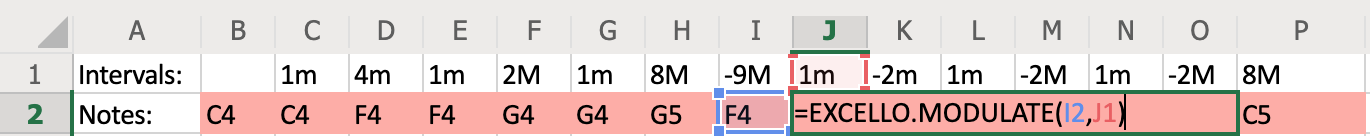
\includegraphics[width=150mm]{figs/modulateFunction.png}}
\caption{Transposing notes using the \texttt{EXCELLO.MODULATE} function.}
\label{implementation:modulateFunction}
\end{figure}

%  \ref{examples}

\subsection{Sustain}

\paragraph{} To prevent confusion between the south instruction and sustains. The symbol ``\texttt{-}" sustains a note. This was chosen because it is light and also has some similarity to a tie.\footnote{A line used in musical notation to increase the length of a note by joining it to another note.} Again, to maintain backwards compatibility, ``\texttt{s}" in a cell is still interpreted as a sustain.

\subsection{Active Turtles}

\paragraph{} To show that active turtle definitions have been recognised, a list of locations of the active turtles is given below the play button. This also helps find spurious turtles not intended to be activated.

\subsection{Automatic Movement}

\paragraph{} To prevent counting the cells in a line, \texttt{m*} instructs a turtle to move as far as there are notes or sustains defined in the direction it is facing. After adding more notes, the turtle instructions do not need editing before pressing play. A part may be meant to finish with a number of rests. As rests are notated with blank cells, a method to extend the path to include these rests was required. A cell can be explicitly defined as a rest with ``\texttt{.}". This is required if multiple turtles are playing a repeating section where one turtle's final cell as a note, sustain or multi-note cell. Without an explicit rest, the turtle would repeat too soon and the parts would consequently be out of phase.

\subsection{Inferred Octave}

\paragraph{} Octave numbers are inferred if omitted. Two methods were considered. Firstly, as most intervals within melodic lines are small, the nearest note could be played.
% This means that a scale would only need the octave defining in the first note.
Whilst this may require the fewest explicit statements of octave numbers, it would be hard to immediately identify the octave of any given note. The last defined octave in the path would need finding and then all subsequent notes walked through keeping track of the octave. The second consideration was to always use the last defined octave. Whilst this may require many octave definitions around the boundary between octaves, it is easier to find the octave of a note by backtracking. The second option was therefore implemented.

\subsection{Chords}

\paragraph{} To aid entering common chords, common types are repeated in a section at the top of the type drop-down. The chord drop-downs layout has been improved with labels to make it clearer what the values refer to. If the notes were entered vertically, the order was reversed, increasing correspondence with traditional staff notation.

\subsection{Activation of turtles}

\paragraph{} A ``Toggle Activation" button was added to the add-in window. When a cell or range is highlighted in the spreadsheet, the activation of any turtle definitions in this range will be toggled when the button is pressed.  This significantly decreases the time to toggle activations, as only two clicks are required, rather than entering the cell edit mode to add or remove an exclamation mark.

\section{Final Prototype Implementation}

\paragraph{} This section discusses the underlying implementation of the final prototype, following the participatory design. Excello consists of three main parts: the turtle system for playing the grid contents, the chord input tool, and the custom Excel functions.

\paragraph{} When the play button is pressed, turtle definitions in the grid are identified. For each, the starting cell and movement instructions are used to establish the contents of the cells it passes through. This is converted to a series of note definitions - pitch, start time, duration, volume. The speed and loop parameters are used to create the structure interpreted by the Tone.js library to schedule and initiate playback. An overview of the data flow and subtasks required to create the musical playback is shown in Figure \ref{fig:overview}.

\begin{figure}[htb]
\begin{center}
  
  \tikzset{every picture/.style={line width=0.75pt}} %set default line width to 0.75pt

  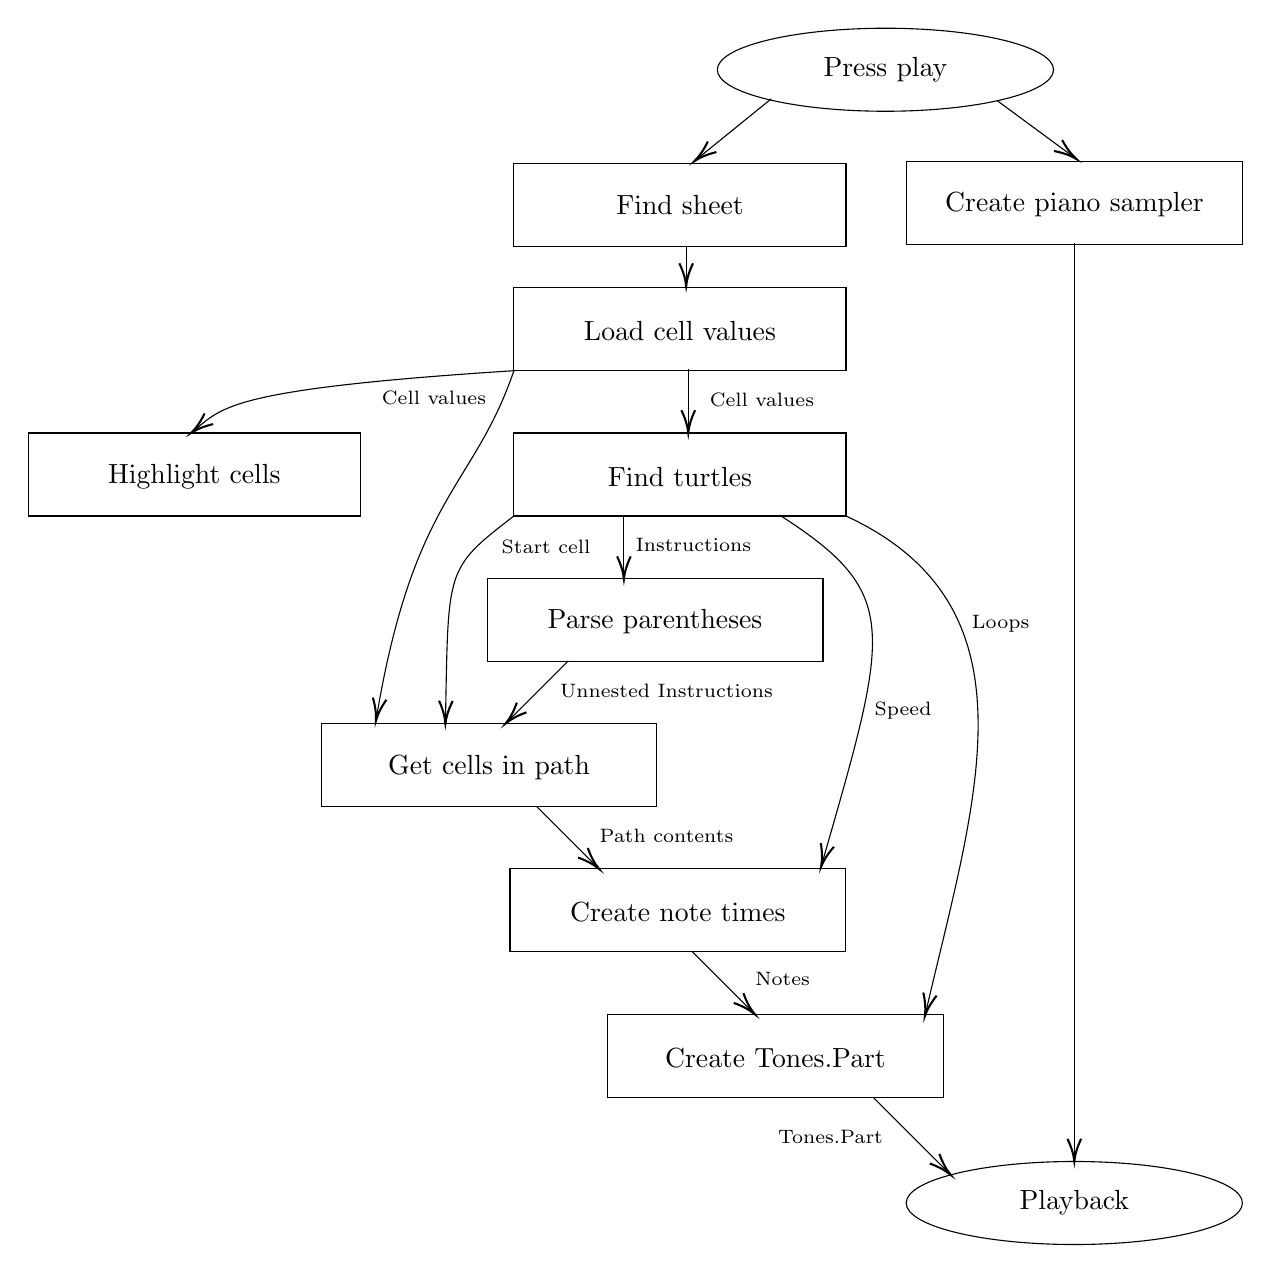
\begin{tikzpicture}[x=0.75pt,y=0.75pt,yscale=-1,xscale=1]
  %uncomment if require: \path (0,604); %set diagram left start at 0, and has height of 604

  %Shape: Rectangle [id:dp3390223975782729]
  \draw   (244.5,71) -- (404.5,71) -- (404.5,111) -- (244.5,111) -- cycle ;

  %Shape: Rectangle [id:dp7168559924493858]
  \draw   (244.5,131) -- (404.5,131) -- (404.5,171) -- (244.5,171) -- cycle ;

  %Shape: Rectangle [id:dp8835932361497658]
  \draw   (433.7,70) -- (595.5,70) -- (595.5,110) -- (433.7,110) -- cycle ;

  %Shape: Rectangle [id:dp9464422191216635]
  \draw   (244.5,201) -- (404.5,201) -- (404.5,241) -- (244.5,241) -- cycle ;

  %Shape: Rectangle [id:dp6384624480751633]
  \draw   (231.6,271) -- (393.4,271) -- (393.4,311) -- (231.6,311) -- cycle ;

  %Shape: Rectangle [id:dp2927464084046889]
  \draw   (151.6,341) -- (313.4,341) -- (313.4,381) -- (151.6,381) -- cycle ;

  %Shape: Rectangle [id:dp9052659554068596]
  \draw   (242.6,411) -- (404.4,411) -- (404.4,451) -- (242.6,451) -- cycle ;

  %Shape: Rectangle [id:dp5637329489183025]
  \draw   (289.6,481) -- (451.4,481) -- (451.4,521) -- (289.6,521) -- cycle ;

  %Curve Lines [id:da3917180624639185]
  \draw    (244.5,241) .. controls (211.17,266.67) and (212.98,265.81) .. (211.52,339.88) ;
  \draw [shift={(211.5,341)}, rotate = 271.14] [color={rgb, 255:red, 0; green, 0; blue, 0 }  ][line width=0.75]    (10.93,-3.29) .. controls (6.95,-1.4) and (3.31,-0.3) .. (0,0) .. controls (3.31,0.3) and (6.95,1.4) .. (10.93,3.29)   ;

  %Straight Lines [id:da6961662223442007]
  \draw    (297.5,241) -- (297.5,269.4) ;
  \draw [shift={(297.5,271.4)}, rotate = 270] [color={rgb, 255:red, 0; green, 0; blue, 0 }  ][line width=0.75]    (10.93,-3.29) .. controls (6.95,-1.4) and (3.31,-0.3) .. (0,0) .. controls (3.31,0.3) and (6.95,1.4) .. (10.93,3.29)   ;

  %Curve Lines [id:da9168950950169605]
  \draw    (372.6,240.6) .. controls (431.31,278.41) and (425.56,294.84) .. (392.99,408.28) ;
  \draw [shift={(392.5,410)}, rotate = 286.01] [color={rgb, 255:red, 0; green, 0; blue, 0 }  ][line width=0.75]    (10.93,-3.29) .. controls (6.95,-1.4) and (3.31,-0.3) .. (0,0) .. controls (3.31,0.3) and (6.95,1.4) .. (10.93,3.29)   ;

  %Curve Lines [id:da7972588626438504]
  \draw    (404.5,241) .. controls (499.03,284.78) and (466.83,377.07) .. (442.86,480.44) ;
  \draw [shift={(442.5,482)}, rotate = 282.99] [color={rgb, 255:red, 0; green, 0; blue, 0 }  ][line width=0.75]    (10.93,-3.29) .. controls (6.95,-1.4) and (3.31,-0.3) .. (0,0) .. controls (3.31,0.3) and (6.95,1.4) .. (10.93,3.29)   ;

  %Straight Lines [id:da6822022155717844]
  \draw    (270.7,310.8) -- (241.91,339.59) ;
  \draw [shift={(240.5,341)}, rotate = 315] [color={rgb, 255:red, 0; green, 0; blue, 0 }  ][line width=0.75]    (10.93,-3.29) .. controls (6.95,-1.4) and (3.31,-0.3) .. (0,0) .. controls (3.31,0.3) and (6.95,1.4) .. (10.93,3.29)   ;

  %Straight Lines [id:da4884596231580207]
  \draw    (255.5,381) -- (284.09,409.59) ;
  \draw [shift={(285.5,411)}, rotate = 225] [color={rgb, 255:red, 0; green, 0; blue, 0 }  ][line width=0.75]    (10.93,-3.29) .. controls (6.95,-1.4) and (3.31,-0.3) .. (0,0) .. controls (3.31,0.3) and (6.95,1.4) .. (10.93,3.29)   ;

  %Straight Lines [id:da9233366942734922]
  \draw    (330.5,451) -- (359.09,479.59) ;
  \draw [shift={(360.5,481)}, rotate = 225] [color={rgb, 255:red, 0; green, 0; blue, 0 }  ][line width=0.75]    (10.93,-3.29) .. controls (6.95,-1.4) and (3.31,-0.3) .. (0,0) .. controls (3.31,0.3) and (6.95,1.4) .. (10.93,3.29)   ;

  %Straight Lines [id:da3670498457872964]
  \draw    (417.5,521) -- (453.49,556.99) ;
  \draw [shift={(454.9,558.4)}, rotate = 225] [color={rgb, 255:red, 0; green, 0; blue, 0 }  ][line width=0.75]    (10.93,-3.29) .. controls (6.95,-1.4) and (3.31,-0.3) .. (0,0) .. controls (3.31,0.3) and (6.95,1.4) .. (10.93,3.29)   ;

  %Straight Lines [id:da28794703530347365]
  \draw    (327.5,111) -- (327.5,128.2) ;
  \draw [shift={(327.5,130.2)}, rotate = 270] [color={rgb, 255:red, 0; green, 0; blue, 0 }  ][line width=0.75]    (10.93,-3.29) .. controls (6.95,-1.4) and (3.31,-0.3) .. (0,0) .. controls (3.31,0.3) and (6.95,1.4) .. (10.93,3.29)   ;

  %Straight Lines [id:da33376731250782754]
  \draw    (328.5,170) -- (328.5,199) ;
  \draw [shift={(328.5,201)}, rotate = 270] [color={rgb, 255:red, 0; green, 0; blue, 0 }  ][line width=0.75]    (10.93,-3.29) .. controls (6.95,-1.4) and (3.31,-0.3) .. (0,0) .. controls (3.31,0.3) and (6.95,1.4) .. (10.93,3.29)   ;

  %Curve Lines [id:da2676626927985757]
  \draw    (244.5,171) .. controls (225.1,227.72) and (196.29,230.77) .. (178.27,338.17) ;
  \draw [shift={(178,339.8)}, rotate = 279.38] [color={rgb, 255:red, 0; green, 0; blue, 0 }  ][line width=0.75]    (10.93,-3.29) .. controls (6.95,-1.4) and (3.31,-0.3) .. (0,0) .. controls (3.31,0.3) and (6.95,1.4) .. (10.93,3.29)   ;

  %Straight Lines [id:da024649031996502035]
  \draw    (514.5,109.6) -- (514.5,550) ;
  \draw [shift={(514.5,552)}, rotate = 270] [color={rgb, 255:red, 0; green, 0; blue, 0 }  ][line width=0.75]    (10.93,-3.29) .. controls (6.95,-1.4) and (3.31,-0.3) .. (0,0) .. controls (3.31,0.3) and (6.95,1.4) .. (10.93,3.29)   ;

  %Shape: Ellipse [id:dp13505581605963868]
  \draw   (433.5,572) .. controls (433.5,560.95) and (469.76,552) .. (514.5,552) .. controls (559.24,552) and (595.5,560.95) .. (595.5,572) .. controls (595.5,583.05) and (559.24,592) .. (514.5,592) .. controls (469.76,592) and (433.5,583.05) .. (433.5,572) -- cycle ;

  %Shape: Ellipse [id:dp006287630832967794]
  \draw   (342.5,26) .. controls (342.5,14.95) and (378.76,6) .. (423.5,6) .. controls (468.24,6) and (504.5,14.95) .. (504.5,26) .. controls (504.5,37.05) and (468.24,46) .. (423.5,46) .. controls (378.76,46) and (342.5,37.05) .. (342.5,26) -- cycle ;

  %Straight Lines [id:da09048722077694915]
  \draw    (368.5,40) -- (333.05,68.74) ;
  \draw [shift={(331.5,70)}, rotate = 320.96000000000004] [color={rgb, 255:red, 0; green, 0; blue, 0 }  ][line width=0.75]    (10.93,-3.29) .. controls (6.95,-1.4) and (3.31,-0.3) .. (0,0) .. controls (3.31,0.3) and (6.95,1.4) .. (10.93,3.29)   ;

  %Straight Lines [id:da9578993167654264]
  \draw    (477.5,41) -- (513.89,67.81) ;
  \draw [shift={(515.5,69)}, rotate = 216.38] [color={rgb, 255:red, 0; green, 0; blue, 0 }  ][line width=0.75]    (10.93,-3.29) .. controls (6.95,-1.4) and (3.31,-0.3) .. (0,0) .. controls (3.31,0.3) and (6.95,1.4) .. (10.93,3.29)   ;

  %Shape: Rectangle [id:dp25073410390478523]
  \draw   (10.5,201) -- (170.5,201) -- (170.5,241) -- (10.5,241) -- cycle ;

  %Curve Lines [id:da2454539812308738]
  \draw    (244.5,171) .. controls (108.92,179.69) and (104.17,188.37) .. (90.53,199.75) ;
  \draw [shift={(89,201)}, rotate = 321.34000000000003] [color={rgb, 255:red, 0; green, 0; blue, 0 }  ][line width=0.75]    (10.93,-3.29) .. controls (6.95,-1.4) and (3.31,-0.3) .. (0,0) .. controls (3.31,0.3) and (6.95,1.4) .. (10.93,3.29)   ;


  % Text Node
  \draw (324.5,91) node  [align=left] {Find sheet};
  % Text Node
  \draw (324.5,152) node  [align=left] {Load cell values};
  % Text Node
  \draw (514.6,91) node  [align=left] {Create piano sampler};
  % Text Node
  \draw (324.5,222) node  [align=left] {Find turtles};
  % Text Node
  \draw (312.5,292) node  [align=left] {Parse parentheses};
  % Text Node
  \draw (232.5,362) node  [align=left] {Get cells in path};
  % Text Node
  \draw (323.5,432) node  [align=left] {Create note times};
  % Text Node
  \draw (370.5,502) node  [align=left] {Create Tones.Part};
  % Text Node
  \draw (514.5,572) node [] [align=left] {\textcolor[rgb]{0,0,0}{Playback}};
  % Text Node
  \draw (260,256) node  [align=left] {{\scriptsize Start cell}};
  % Text Node
  \draw (331,255) node  [align=left] {{\scriptsize Instructions}};
  % Text Node
  \draw (432,335) node  [align=left] {{\scriptsize Speed}};
  % Text Node
  \draw (479,293) node  [align=left] {{\scriptsize Loops}};
  % Text Node
  \draw (318,325) node  [align=left] {{\scriptsize Unnested Instructions}};
  % Text Node
  \draw (318,395) node  [align=left] {{\scriptsize Path contents}};
  % Text Node
  \draw (374,464) node  [align=left] {{\scriptsize Notes}};
  % Text Node
  \draw (397,540) node  [align=left] {{\scriptsize Tones.Part}};
  % Text Node
  \draw (206,184) node  [align=left] {{\scriptsize Cell values}};
  % Text Node
  \draw (423.5,26) node [] [align=left] {Press play};
  % Text Node
  \draw (364,185) node  [align=left] {{\scriptsize Cell values}};
  % Text Node
  \draw (90.5,222) node  [align=left] {Highlight cells};


  \end{tikzpicture}

\end{center}
\caption{An overview of the playback algorithm and dataflow of Excello\label{fig:overview}}
\end{figure}

\paragraph{} The \texttt{Sampler} is an extension of the \texttt{Tone.Instrument} class. This interpolates between pitched samples to create arbitrary notes. A sampler is loaded using the Salamander grand piano samples~\footnote{https://freepats.zenvoid.org/Piano/acoustic-grand-piano.html} which includes four pitches (out of a possible 12) per octave. This accurately interpolates notes whilst reducing loading times and storage requirements.

\subsection{Identifying Cells}

\paragraph{} A drop-down is populated with names loaded using the Office API. Having pressed play, the cell values from the selected sheet are loaded and then analysed for highlighting and calculating the musical output. Cells containing at least one note definition are highlighted red. A note must contain a note name, optional accidental, optional octave number, and optional volume instruction following a space. This is a dynamic marking or number between 0 and 1. Notes are identified using the following regular expression:

\begin{verbatim}
^[A-G](#|b|)?[1-9]?( (0(\.\[0-9]+)?|1(\.0)?|ppp|pp|p|mp|mf|f|ff|fff))?$
\end{verbatim}

\paragraph{} Cells containing multiple definitions (e.g. ``\texttt{C4 ff,-, ,D}", ``\texttt{,,G,F$\sharp$}") are split using commas. The resulting strings are trimmed of starting and ending whitespace and then must either be a note, sustain (``\texttt{-}" or ``\texttt{s}"), explicit rest (``\texttt{.}") or empty string (created from trimming a rest). Cells matching ``\texttt{-}",``\texttt{.}" or ``\texttt{s}" are highlighted a lighter red. Turtle definitions (e.g. ``\texttt{!turtle(B2:B4, r m*, 200, 1)}") are identified using:
\begin{verbatim}
^(!turtle\().*(\))$
\end{verbatim}
and these cells are highlighted green. The addresses of cells containing a turtle definition are added to the live turtle section of the add-in window.

\subsection{Parsing Movement Instructions}

\paragraph{} Movement instructions are converted to a single unnested list of commands (e.g.~``\texttt{(r m2)2}" becomes ``\texttt{[r, m2, r, m2]}") so the turtle's path can be established. The \texttt{parse} method of the Parenthesis\footnote{https://www.npmjs.com/package/parenthesis} library seemed suitable for aiding this string manipulation. This parses strings containing brackets into a nested array. For example, \texttt{parse(\textcolor[rgb]{0,0.7,0}{\upquote{a(b[c\{d\}])}})} gives \texttt{[\textcolor[rgb]{0,0.7,0}{\upquote{a(}}, [\textcolor[rgb]{0,0.7,0}{\upquote{b[}}, [\textcolor[rgb]{0,0.7,0}{\upquote{c\{}}, [\textcolor[rgb]{0,0.7,0}{\upquote{d}}], \textcolor[rgb]{0,0.7,0}{\upquote{\}}}], \textcolor[rgb]{0,0.7,0}{\upquote{]}}], \textcolor[rgb]{0,0.7,0}{\upquote{)}}]}.

\paragraph{} This suggests the string ``\texttt{(r m2)2}" would become \texttt{[\upquote{(}, [\upquote{r m2}], \upquote{)2}]}. By removing the brackets from these strings, a simple recursive method could be built to output \texttt{\upquote{r m2 r m2}} from \texttt{[[\upquote{r m2}], \upquote{2}]}. However, upon testing this, the library outputted an undefined array. From investigating the source code, I established that strings with a number following a closing parenthesis all produced this error. Substituting characters for the numbers or placing a symbol before all numbers and then later removing these would allow the library to be used. Instead, using the Parenthesis method as inspiration, I implemented my own parsing function tailored to Excello.

\paragraph{} This has two main steps. First, the deepest bracketed expression is stored in an array with the brackets removed. This expression is replaced in the original string with the string \upquote{\texttt{\_\_\_}$x$\texttt{\_\_\_}} where $x$ is the expression's index in the array. This is repeated until the string contains no brackets. Then a recursive function uses the values of $x$ to reconstruct the string in the nested array format. This method is outlined in Algorithm \ref{alg:parenthesis}. The Typescript implementation is in Appendix \ref{appendix:parseBrackets}.

\begin{algorithm}[!htp]
\caption{Parsing bracketed expression. \texttt{str.replace(regex,f)} (line 13) performs \texttt{f(s)} on the first substring, \texttt{s}, of \texttt{str} matching the regular expression \texttt{regex}.}
\label{alg:parenthesis}
\begin{algorithmic}[1]
\Procedure{parseBrackets}{$str$}

   \State $idPadding\gets \texttt{\upquote{\_\_\_}}$
   \State $unnestedStr\gets []$
   \State $deepestLevelBracketsRE\gets \texttt{RegExp(\upquote{\textbackslash\textbackslash([\^{}\textbackslash\textbackslash(\textbackslash\textbackslash)]*\textbackslash\textbackslash)})}$
   \State $replacementIDRE\gets \texttt{RegExp(\upquote{\textbackslash\textbackslash} + }idPadding\texttt{ + \upquote{([0-9]+)} + }idPadding\texttt{)}$\\

   \Procedure{replaceDeepestBracket}{$x$}
     \State \texttt{unnestedStr.push(x.substring(1, x.length-1))}
     \State \texttt{\textbf{return} idPadding + (unnestedStr.length - 1) + idPadding}
   \EndProcedure \\

   \While{\texttt{deepestLevelBracketsRE.test(str)}}
     \State \texttt{str = str.replace(deepestLevelBracketsRE,replaceDeepestBracket)}
   \EndWhile

   \State \texttt{unnestedStr[0] = str}\\

   \Procedure{reNest}{$outerStr$}
     \State $renestingStr\gets []$
     \While{There is a match of $replacementIDRE$ in $outerStr$}
       \State $matchIndex\gets$ index of the match in $outerStr$
       \State $matchID\gets$ ID of the match (number between padding)
       \State $matchString\gets$ matched string\\

       \If{$matchIndex >$ 0}
				\State $renestingStr$.push($outestStr$.substring(0, $matchIndex$))
			\EndIf
			\State $renestingStr$.push(reNest($unnestedStr$[$firstMatchID$]))
			\State $outestStr$ = $outestStr$.substring($matchIndex$ + $matchString$.length)
     \EndWhile
     \State $renestingStr$.push($outestStr$)
     \State \textbf{return} $renestingStr$
   \EndProcedure \\

   \State \textbf{return} \textsc{reNest}($unnestedStr$[0])

\EndProcedure
\end{algorithmic}
\end{algorithm}


\paragraph{} Having submitted a bug report on the Parenthesis GitHub, and implemented my own method for parsing turtle movement instructions, I implemented a fix to the Parenthesis library. The library previously performed replacements with the string \upquote{\texttt{\_\_\_}$x$}. $x$ and following numbers would concatenate forming a single number, causing the library to fail. My method of having an identifier before and after $x$ fixed this issue. I also added additional tests to Parenthesis to verify my method and ensure that previous tests all passed before submitting a pull request. I have made an open source contribution, as this has since been merged into the library and published.

\paragraph{} I wrote an additional recursive method to unnest the array into a single stream of commands. An empty string, \texttt{s}, is initialised. For each item in the array, if it is an array, unnest the contents recursively and add the result to s. If not, it will be one or more single movement commands. If the single movement commands start with a number, the result is added to \texttt{s} that number of times. The remaining instructions are added to \texttt{s}. This is outlined in Algorithm \ref{alg:unnest}. The implementation is shown in Appendix \ref{appendix:processParsedBrackets}.

\begin{algorithm}[!htbp]
\caption{Unnesting parsed bracketed expressions.}
\label{alg:unnest}
\begin{algorithmic}[1]
\Procedure{processParsedBrackets}{$arr$}

   \State $s\gets \texttt{\upquote{}}$
   \State $previousArr$

   \For{$v$ in $s$}
    \If{$v$ is an array}
     \State $previousArr \gets$ processParsedBrackets($v$)
    \Else
       \If{previous instruction was an array}
        \State $s \gets s + previousArr$
        \If{next instruction is a number}
          \State $s \gets s + previousArr$, that number of times minus one
        \EndIf
       \EndIf
       \State $s \gets s + $ remaining instruction in $v$
    \EndIf
   \EndFor
   \State \textbf{return} $s$

\EndProcedure
\end{algorithmic}
\end{algorithm}

\subsection{Getting Cells in Turtles' Paths}

\paragraph{} If the turtle's first argument defines a range of starting cells, the cell addresses of this range are calculated. For each starting cell, the unnested instructions and sheet values are used to find the contents of the cells the turtle passes through. This process models the movement of the turtle within the grid, keeping track of its position and the direction in which it is facing. For each instruction, the position and direction are updated as required, and the contents of any new cells entered are added to a list of notes.

\paragraph{} For the ``\texttt{m*}" instruction, the number of steps the turtle takes must be computed. Given the turtle's current position and direction, the one-dimensional array of cells in front of it is taken. The turtle should step to the last cell that defines a note, sustain or explicit rest. The number of steps is the array's length minus the index of the first element in the reversed array satisfying this criterion.

\subsection{Creating Note Times}

\paragraph{} The cells a turtle moves through are used to create a data structure containing the information for playback using the Tone library. For each turtle, the following array is produced: \texttt{[[<Note 1>,...,<Note N>], <number of cells>]} (note sequence array). Each note is as follows: \texttt{[<start time>, [<pitch>, <duration>, <volume>]]}. Volume and octave are added to each note if they were omitted from a cell.

\paragraph{} The Tone Transport is a timeline along which events can be scheduled. This supports many different representations of time. I used Transport Time for all note onsets and durations. This is of the form \texttt{\upquote{BARS:QUARTERS:SIXTEENTHS}} where the three values are numbers and can be non-integer. With \texttt{QUARTERS} representing the number of cells, the calculation of exact times, or arbitrary musical notes can be avoided. This allows the contents of cells to be easily converted to times to be interpreted by the Tones library.

\paragraph{} The note sequence array is initiated by counting the notes that are defined in the cell contents using regular expressions for identifying notes and multi-note cells. The cells are iterated through keeping track of the active note and adding it to the note sequence when it ends. Outside of this loop, variables track how many cells and notes through the process the algorithm is and whether it is currently a rest or note. Variables keep track of the note currently being played - when it started (\texttt{currentStart}), the pitch (\texttt{currentNote}) and the volume (\texttt{currentVolume}). As volume and octave number may be omitted, variables also keep track of these. Table \ref{tab:times} outlines the actions performed when a cell is read. Notes are added to the note sequence in the form \texttt{[currentStart, [currentNote, \upquote{0:} + noteLength + \upquote{:0}, currentVolume]]}.

\begin{table}[ht]
\begin{tabular}{|l|l|l|l|l|}
  \hline
  \textbf{Cell}&\textbf{State}&\multicolumn{3}{c|}{\textbf{Action}} \\
  \hline
  \multirow{5}{*}{Note}&\multirow{3}{*}{Note}&Note, octave and &Previous note added&currentStart = \\
  &&volume established&to note sequence&\upquote{0:}+beatCount+\upquote{:0}\\
  &&from cell contents&&currentNote = value\\
  \cline{2-2}
  \cline{4-4}
  &\multirow{2}{*}{Rest}&and previous values&inRest = false&noteLength = 1\\
  &&&&currentVolume = volume\\
  \hline
  \multirow{2}{*}{Sustain}&Note&\multicolumn{3}{l|}{noteLength++}\\
  \cline{2-5}
  &Rest&\multicolumn{3}{l|}{Nothing (has no semantic value)}\\
  \hline
  \multirow{3}{*}{Rest}&\multirow{2}{*}{Note}&\multicolumn{3}{l|}{Previous note added to note sequence}\\
  &&\multicolumn{3}{l|}{inRest = true}\\
  \cline{2-5}
  &Rest&\multicolumn{3}{l|}{Nothing}\\
  \hline
\end{tabular}
\caption{The actions taken when processing each cell to create note times. The beat count corresponds to the cell number being processed and is incremented each time.\label{tab:times}}
\end{table}
\vspace{-10pt}

\paragraph{} The same method is used for multi-note cells, except the note length and cell count are incremented by the appropriate fraction for each item in the cell. If, after the final cell, the state is a note, it is ended and added to the note sequence.

\paragraph{} The values in the note sequence are sufficient for the piano sampler to play a note using the \texttt{triggerAttackRelease} function. The \texttt{Tone.Part} class allows multiple calls to this method to be defined, started, stopped and looped as a single unit. This is defined with the note sequence and its speed set with the evaluated turtle speed argument. The number of cells, calculated when creating the note times, number of repeats, and the evaluated speed argument are used to control when looping ends.

% \begin{verbatim}
% var turtlePart = new Tone.Part(function(time, note){
%   piano.triggerAttackRelease(note[0], note[1], time, note[2]);
% }, noteTimes).start();
% if (repeats>0){
%   turtlePart = turtlePart.stop("0:" + (repeats*beatsLength/speedFactor) + ":0");
% }
% turtlePart.loop = true;
% turtlePart.loopEnd = "0:" + beatsLength + ":0";
% turtlePart.playbackRate = speedFactor;
% \end{verbatim}

% \begin{lstlisting}[style=js]
%   var turtlePart = new Tone.Part(function(time, note){
%     piano.triggerAttackRelease(note[0], note[1], time, note[2]);
%   }, noteTimes).start();
%   if (repeats>0){
%     turtlePart = turtlePart.stop("0:" + (repeats*beatsLength/speedFactor) + ":0");
%   }
%   turtlePart.loop = true;
%   turtlePart.loopEnd = "0:" + beatsLength + ":0";
%   turtlePart.playbackRate = speedFactor;
% \end{lstlisting}

\subsection{Chord Input}\label{Chord Input}

\paragraph{} The next two subsections (\S\ref{Chord Input} and \S\ref{Custom Excel Functions}) outline the two smaller parts of the Excello; the chord input tool, and the custom Excel functions. When the insert button in the add-in window is pressed, the note, type, inversion and octave of the chord are extracted from their HTML elements. The chord interface within the add-in window is shown in Figure \ref{fig:chordInput}. The tonal library is used to generate the chord notes:

\begin{verbatim}
var chordNotes = Chord.notes(chordNote, chordType).map(x => Note.simplify(x));
\end{verbatim}
\vspace{-10pt}

\begin{figure}[htb]
\centerline{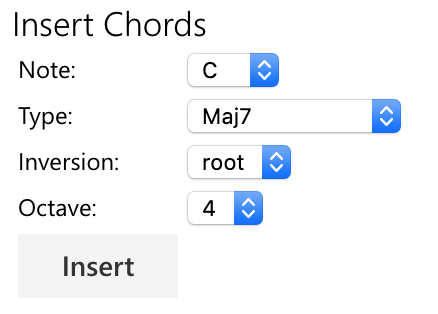
\includegraphics[width=50mm]{figs/insertChord.png}}
\caption{The interface within the add-in window for inserting the notes of chords.}
\label{fig:chordInput}
\end{figure}

\vspace{-20pt}
\paragraph{} The tonal \texttt{simplify} function reduces note definitions to contain at most one accidental, as required by Excello. This provides a list of notes in ascending order, without octaves or taking into account the inversion. To create the correct inversion of the chord, the array of notes is rotated by the inversion number.

\paragraph{} The given octave number is appended to the first note. A dictionary matches note names, accounting for enharmonics,\footnote{Notes that are the same pitch but different names, such as A$\flat$ and G$\sharp$.} to position in the chromatic scale starting at C (the first note of the octave in SPN). For each preceding note, if it appears in an equal or lower position in the scale than its predecessor, the octave number is incremented before appending. Otherwise, it is in the same octave, so the octave number is appended without modification.

\paragraph{} The selected range is acquired with the Office API. The chord notes are entered starting at the top-left corner of this range. If the range's height is greater or equal to its width, the notes are entered vertically going down. Otherwise, they are entered horizontally going right. Using the Office API, the range is set to the 2D array where the chord is entered.

\subsection{Custom Excel Functions}\label{Custom Excel Functions}

\paragraph{} Custom functions are implemented using another add-in. Rather than a separate window like the main Excello add-in, additional functions can be used in cells with the prefix ``\texttt{=EXCELLO.}". The file structure was generated with the Yeoman generator. The name, description, result type, and parameter names and types are stored in a JSON schema. This is used by Excel to provide argument prompts and autofill when writing formulae. Functions are defined in Typescript.

\paragraph{} The turtle function concatenates the arguments into the Excello turtle format. Other cells can be referenced, for example, the speed variable can reference a global tempo variable as in Figure \ref{implementation:turtleFunction}.

\paragraph{} The modulation function separates the note and volume for every note defined in a cell. The note is modulated using the tonal \texttt{Distance.transpose} function and recombined with the volume. The drag fill feature of Excel can be employed by the user to transpose sections or define melodic lines using the interval between notes as in Figure \ref{implementation:modulateFunction}.

\section{MIDI Converter}

\paragraph{} This section explains the Python converter from MIDI to CSV for Excello playback. A MIDI file is divided into up to 16 parallel tracks~\cite{midiSpec}. Each track contains a series of messages defined using predefined status and data bytes. I used the Mido library\footnote{https://mido.readthedocs.io/en/latest/index.html} to read MIDI files and abstract away from the underlying byte representations to view the messages. Note onsets and offsets are two separate events with two separate messages~\cite{midiSpec}. These messages include the note pitch, velocity, channel (not relevant) and time in ticks since the last message~\cite{midoSpec}.

\paragraph{} First, the list of messages is converted to a list of notes defined by onset and offset time, pitch and velocity. For each track, the messages are iterated through, using the time value in every message (including control and meta messages) to update a variable tracking time. For note onset messages, this is added to a dictionary mapping pitch to a list of currently active note start times. Lists are used because a pitch can be active multiple times at once. For note offset messages, or onset messages with zero velocity, the note popped from the active notes at that pitch with end time added is added to the list of all notes defined in the file.

\paragraph{} As each turtle only plays one note at a time, the notes are split into lists so no list contains concurrently played notes. Provided the initial list of notes is non-empty, a new list is created. The first remaining note is moved to the new list. Then iterating over the remaining notes, the next note starting after the previous note ends is moved to this new list. The number of iterations required is the number of turtles, $n$.

\paragraph{} If every tick corresponds to a cell, any combination of note onsets and offsets in a MIDI file can be accurately represented in Excello. To achieve smaller representations, the start and end times are converted to smaller cell numbers within the path of the turtle. For many MIDI files, the duration of a note is different from the time it occupies in notation. For example, a note immediately followed by another note in notation may have an end time significantly less than the start time of the next note in MIDI. A method is required to account for this. For all notes, before creating the different turtle streams, the length of the notes in ticks and differences between consecutive start times are found. The minimum value greater than 1 or modal value for these times are calculated depending on the compression level giving the $lengthStat$ and $di\hspace{-0.1em}f\hspace{-0.2em}f\hspace{-0.1em}erenceStat$.
\vspace{-10pt}

  $$ratio_{int} = \lfloor\max(lengthStat, di\hspace{-0.1em}f\hspace{-0.2em}f\hspace{-0.1em}erenceStat)/\min(lengthStat, di\hspace{-0.1em}f\hspace{-0.2em}f\hspace{-0.1em}erenceStat)\rfloor$$
  % $$ratio_{int} = \lfloor ratio \rfloor$$
  % $$correction = ratio/ratio_{int}$$
For each note, the times are adjusted as follows:
  $$length \gets (start - end) / lengthStat \text{ (rounded to the nearest 0.1)}$$
  $$start \gets start / di\hspace{-0.1em}f\hspace{-0.2em}f\hspace{-0.1em}erenceStat \times ratio_{int} \text{ (rounded to the nearest 0.1)}$$
  $$end \gets start +length$$

\paragraph{} The streams, with note start and end times corresponding to cells, are converted to a CSV file for Excello. Each turtle's path is initialised as an array of empty strings with length equal to the maximum end time for a note in any turtle, $L$. Each note the turtle plays is entered into the array. MIDI defines pitch using the integers. As there are 12 notes in an octave, modulus and division with 12 gives the note name and octave for SPN. If velocity is different from the previous note played by the turtle (or the note is the first note), the eight-bit MIDI velocity is mapped to Excello's [0,1] range. If the note length is greater than one, sustains are placed in the following cells. These paths go right starting in column A, with the first in row 2.

\paragraph{} Finally, the turtle definition is placed in the spreadsheet. The start cell range is ``A2:A$(n+1)$". The movement instruction is ``r m$L$". The MIDI file contains meta data for the \texttt{tempo} (milliseconds per beat) and \texttt{ticks\_per\_beat}. Cells per minute is calculated as follows:
$$cells\ per\ tick \times ticks\ per\ beat \times beat\ per\ minute$$
$$= \frac{ratio_{int}}{di\hspace{-0.1em}f\hspace{-0.2em}f\hspace{-0.1em}erenceStat} \times \texttt{ticks\_per\_beat} \times \frac{60 \times 10^6}{\texttt{tempo}}$$
With a value of 1 for repeats, the turtle definition is put in cell A1 and the CSV exported.

\newpage
\section{Repository Overview}

\tikzstyle{dir}=[draw=black,thick,anchor=west]
\tikzstyle{src}=[draw=black,thick,anchor=west,fill=red!30]
\tikzstyle{file}=[draw=black,thick,anchor=west,draw=none]

\begin{wrapfigure}{r}{8cm}
\vspace{-15pt}
% \begin{figure}[tbh]
\begin{tikzpicture}[%
  grow via three points={one child at (0.5,-0.7) and
  two children at (0.5,-0.7) and (0.5,-1.4)},
  edge from parent path={(\tikzparentnode.south) |- (\tikzchildnode.west)}]
  \node [dir] {Excello}
    child { node [dir] {Excel Music}
      child { node [dir] {assets}}
      child { node [dir] {node\_modules}}
      child { node [dir] {src}
        child { node [file] {index.ts}}
        child { node [file] {turtle.ts}}
        child { node [file] {chords.ts}}
        child { node [file] {regex.ts}}
        child { node [file] {conversions.ts}}
        child { node [file] {bracketsParse.ts}}
      }
      child [missing] {}
      child [missing] {}
      child [missing] {}
      child [missing] {}
      child [missing] {}
      child [missing] {}
      child { node [file] {index.html}}
      child { node [file] {manifest.xml}}
    }
    child [missing] {}
    child [missing] {}
    child [missing] {}
    child [missing] {}
    child [missing] {}
    child [missing] {}
    child [missing] {}
    child [missing] {}
    child [missing] {}
    child [missing] {}
    child [missing] {}
    child { node [dir] {CustomFunctions}
      child { node [dir] {src}
        child { node [file] {excello.ts}}
      }
      child [missing] {}
      child { node [dir] {config}
        child { node [file] {excello.json}}
      }
      child [missing] {}
      child { node [dir] {node\_modules}}
      child { node [file] {manifest.xml}}
    }
    child [missing] {}
    child [missing] {}
    child [missing] {}
    child [missing] {}
    child [missing] {}
    child [missing] {}
    child { node [dir] {MIDI}
      child { node [file] {MIDI\_Conversion.ipynb}}
    };
\end{tikzpicture}
\caption{File structure overview showing original files}
\label{fig:repo}
\vspace{-30pt}
% \end{figure}
\end{wrapfigure}

\paragraph{} Figure \ref{fig:repo} shows a reduced project file structure including all original source code. Excel Music is the add-in that parses the notation and produces music. Both this and CustomFunctions were generated using the Yeomann generator. The manifest.xml files are added to Excel and point to the resources to run the add-in. Users were given a different manifest pointing to a distribution hosted online with Surge. node\_modules contains all libraries required to run the add-ins and is managed using npm.

\paragraph{} The index.html file defines the window that appears on the right of the spreadsheet. assets contains the piano samples. index.ts defines what happens when the buttons of the window are pressed and imports from the remaining Typescript files. turtle.ts contains all the code to produce musical output from the spreadsheet, with helper functions in regex.ts, conversions.ts and bracketsParse.ts. bracketsParse.ts was based on Parenthesis which was initially incompatible for Excello's needs. chords.ts is for inserting chord notes into the grid.

\paragraph{} customFunctions.ts contains the implementation of EXCELLO.TURTLE and EXCELLO.MODULATE. The index.html file created when generating this add-in is not seen by the user so was not re-written.

\paragraph{} The Python notebook MIDI\_Conversion.ipynb converts MIDI files to the Excello notation. Conversions of MIDI corpora are included in the MIDI directory.

\paragraph{} I shall release Excello as an open source project under the MIT license. This is compatible with the MIT licenses of the libraries. The Salamander piano samples come under a creative commons license\footnote{https://creativecommons.org/licenses/by/3.0/.} so credit shall be given in the Excel add-in window.



%TC:group tabular 1 1
%TC:group table 1 1

\chapter{Implementation}

\paragraph{} This chapter shall explain how turtles are defined, and covers the remaining features of the initial prototype. The format and results of formative evaluation using this initial prototype shall be summarised, and the design decisions and changes that were made to Excello during the participatory design process will be discussed. Then, the technical details of Excello and the MIDI to Excello converter will be explained. It concludes with an overview of the project repository.

\section{Initial Prototype}

\begin{figure}[tbh]
\centerline{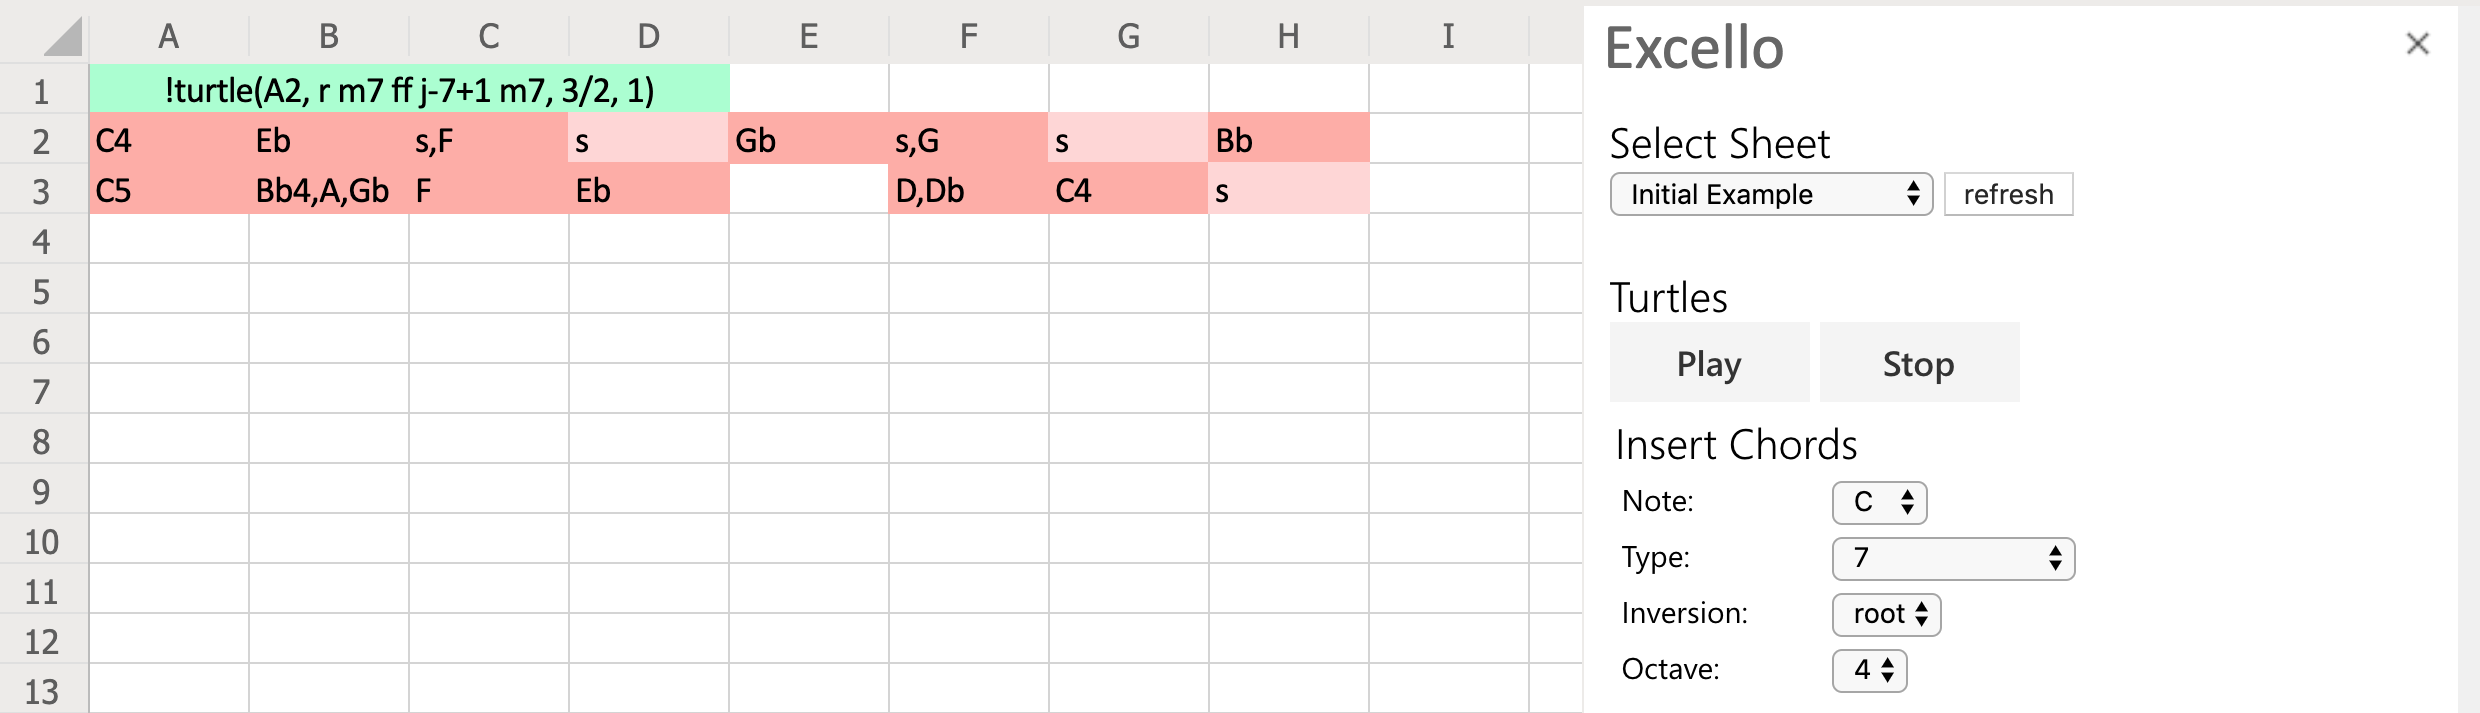
\includegraphics[width=150mm]{figs/initialPrototype.png}}
\caption{A two line motif defined in the initial Excello prototype}
\label{implementation:initialPrototype}
\end{figure}
\begin{figure}[tbh]
\centerline{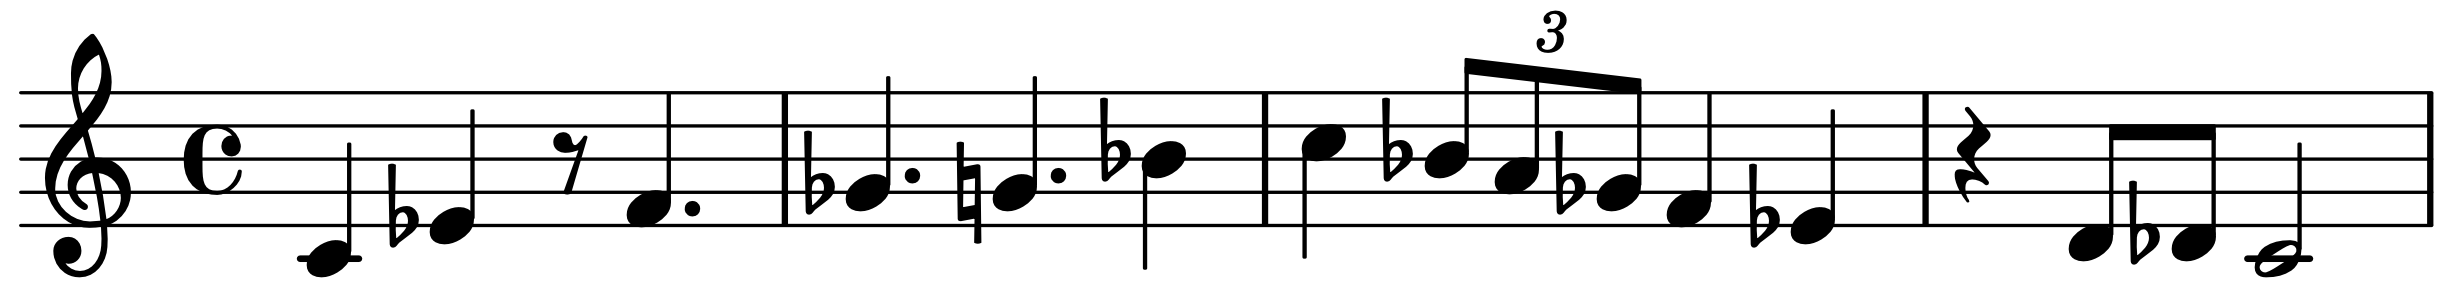
\includegraphics[width=150mm]{figs/initialScore.png}}
\caption{The notes played by the turtle in Figure \ref{implementation:initialPrototype}}
\label{implementation:initialScore}
\end{figure}

\vspace{-10pt}
\paragraph{} Notes and turtles can be defined in any cell. Turtles' interpretation of cells is shown in Table \ref{tab:cells}. When the Excello add-in is opened, a window opens on the right side of Excel as shown in Figure \ref{implementation:initialPrototype}. The melodic line produced is shown in figure \ref{implementation:initialScore}. Play and stop buttons launch all the turtles defined in the spreadsheet and initiate playback with a realistic piano sound.

\begin{table}[htb]
\centering
% \caption{Grammar Rules for the turtle movement instructions. $z \in \Z$}
\vspace{1pt}
\begin{tabular}{|l|l|} \hline
\textbf{Interpretation}&\textbf{Format}\\ \hline
Note& Name (A-G), optional accidental and octave number e.g.~\texttt{F$\sharp$4}\\ \hline
Sustain& \texttt{s}\\ \hline
Multiple notes& Notes, rests or sustains separated by a comma. Rests \\
subdivided in time& must be a space or an empty string e.g.~\texttt{E4,,C4,s}\\ \hline
Rest& Any cell not interpreted as a note, sustain or multi-note. \\ \hline
\end{tabular}
\caption{Interpretation of cells.\label{tab:cells}}
\end{table}

\subsection{Turtles}

\paragraph{} The following formula is enetered into a cell in the grid to define a turtle:\\
\texttt{!turtle(<Starting Cell>, <Movement>, <Speed>, <Number of Loops>)}

\vspace{-5pt}
\subsubsection{Activation}

\paragraph{} The prefix ``\texttt{!}" indicates the turtle will be activated when the play button is pressed. Just as digital audio workstations allow track muting and soloing, this can be used to modify which turtles play, without losing their definitions.

\vspace{-5pt}
\subsubsection{Starting Cell}

\paragraph{} The turtle's starting cell (\texttt{A2} in Figure \ref{implementation:initialPrototype}), which is also played, is a cell reference. As with Excel formulae, this is a concatenation of letters for the column and numbers for the row.

\paragraph{} As each turtle only plays one note at a time, multiple turtles must be defined to play polyphonic music such as chords. It was believed that users would define turtles following identical paths but in adjacent rows or columns. Multiple turtles following identical paths but starting from adjacent cells are defined using the existing Excel range notation for the starting cells. ``\texttt{A2:A5}" would define four turtles in the cells A2,A3,A4,A5. This prevents writing multiple turtle definitions differing in only the start cell row.

\vspace{-5pt}
\subsubsection{Movement}

\paragraph{} Turtles start facing north. The language for programming turtle movement is discussed in the Preparation chapter. The instructions are \texttt{r m7 ff j-7+1 m7} in Figure \ref{implementation:initialPrototype}. Using brackets to repeat movements had not been implemented by the start of the participatory design process.

\vspace{-5pt}
\subsubsection{Speed}

\paragraph{} An optional third argument is the speed of the turtle relative to 160 cells per minute. The default, 1, corresponds to 160 cells per minute. ``\texttt{3/2}", as in Figure \ref{implementation:initialPrototype}, would move the turtle at 240 cells per minute. Relative speed was used so it would be easier to tell the speed relation between turtles. This particularly suits phase music. Arbitrary maths can be provided, allowing turtles' speeds to be irrational multiples of each other.

\vspace{-5pt}
\subsubsection{Number of Loops}

\paragraph{} An optional fourth argument defines the number of repetitions of the turtle's entire path (\texttt{1} in Figure \ref{implementation:initialPrototype}). By default, the turtle loops infinitely. Repeating parts (e.g.~the cello in Pachelbel's Canon in D) therefore only need defining once.

\subsection{Highlighting}

\paragraph{} To assist recognising notes and turtles, when the play button is pressed, cells are highlighted. Activated or deactivated turtle definitions are highlighted green. Cells containing definitions of notes, or multiple notes, are highlighted red. Sustain cells are highlighted a lighter red, showing correspondence to notes whilst maintaining differentiation.

\subsection{Chord Input}

\paragraph{} To use the musical abstractions of chords whilst keeping the paradigm that a turtle is responsible for up to one note at any time, a tool to add chords is included. The note, type, inversion\footnote{Which note of the chord comes first, the other notes ascend from this. This is much like list rotations.} and starting octave of the chord are input into four drop-downs. The insert button enters the notes of the chord into the grid. If a single cell or a range taller than it is wide is highlighted in the spreadsheet, the notes are inserted vertically starting at the top-left of the range. Otherwise, the notes will be inserted horizontally. Whether the turtles are moving horizontally or vertically both chords and arpeggios\footnote{Where the notes of a chord are played individually in rising or descending order.} can be easily defined. Thus, helpful musical abstractions are still available whilst keeping the cleanness of the turtle system.

\section{Formative Evaluation}

\paragraph{} To guide development to best suit users, participants were involved in formative evaluation. Twenty-one University of Cambridge students, across a range of subjects, took part in the participatory design process. Initially, one-on-one tutorials on the initial prototype were given, followed by a short exercise. After these, users were interviewed on how they found Excello, drawing particular attention to actions that they found particularly unintuitive or requiring notable mental effort. Comparisons were made to musical interfaces with which participants were already familiar. The ethical and data handling procedures are discussed in the evaluation chapter.

\paragraph{} To realistically simulate how Excello would be used, participants carried out an exercise of their choice. Often this was transcribing a piece from memory or from traditional notation into the Excello notation. Two exercises were provided if participants had no immediate inspiration; transcribing a piece from western notation or changing existing Excello notation.

\paragraph{} These sessions were carried out in January 2019. Participants were asked to continue using Excello until the summative evaluation sessions in March. Additional feedback was collected as participants used Excello in their own time. This also ensured the summative evaluation was done with users that had sufficient experience of the interface.
% Participants were encouraged to get in contact with any additional issues or suggestions they had during this time.

\subsection{Issues and Suggestions}

\paragraph{} The issues and suggestions from the participatory design process are summarised below.

\subsubsection{Turtle Notation}

\paragraph{} Dynamics in the turtle instructions (e.g. \texttt{ppp m p m mf m ff m}) made establishing the turtle's path harder, as not all commands related to movement (``\texttt{m4}"). As the dynamics weren't next to the notes to which they corresponded, knowing the volume of a note or where to place the dynamics within the turtle to apply to notes in the spreadsheet was challenging. The initial prototype had no way to assign a dynamic to notes in the first cell. The starting cell could be empty, but this was inconvenient for looping parts, as this empty cell would be included in the loop. Users not familiar with western notation dynamics found them unintuitive. Furthermore, these discrete markings do not enable a continuous volume scale.

\paragraph{} When transcribing a piece, dividing its tempo by 160 for the relative speed caused unnecessary work. Users also forgot whether relative speed referred to the time spent in each cell or how quickly the turtle moved. Following the tutorial, users often had to check the position and meaning of turtle arguments.

\paragraph{} As the number of dynamics and movement commands grew, instructions became long and establishing turtle behaviour became cognitively challenging. Some users confused the ``\texttt{s}" within the turtle instructions to mean sustain (as it does in cells) and not south.

\subsubsection{Feedback}

\paragraph{} It was often unknown if pressing play actually registered, especially if the workbook saving delayed Excello's access to the spreadsheet. If a turtle had accidentally been left activated (with ``\texttt{!}"), the entire grid required searching to locate it. Users requested a summary of active turtle locations in addition to the highlighting.

\subsubsection{MIDI conversions}

\paragraph{} Users of production software said importing and exporting MIDI files would be helpful. If working with an existing MIDI file, converting that into the Excello notation would be convenient. Exportation would let Excello be used to create chord sequences, bass lines and the piece structure, before adding additional effects and recording in digital audio work stations.

\subsubsection{Sources of effort when writing}

\paragraph{} After inputting notes into the grid, the number of cells the turtle had to move required counting. As these were often in a straight line, the Excel status bar allowed users to select cells and immediately see how many there were. However, this was still not efficient, and was particularly inconvenient when users were writing notes and periodically testing what they had written so far. Some users instructed turtles to move forward significantly more steps than required to prevent counting. This is not feasible for looping parts. It was suggested that turtles could determine independently how far they should move.

\paragraph{} Instructions with repeated movements such as moving to the end of a line and jumping down to the beginning of a line below, required a lot of repetition.

\paragraph{} Many of the notes in melodic lines are frequently in the same octave. As such, repeatedly writing out the octave number was tiresome. One user made a comparison to LilyPond~\cite{sandberg:lily} where if the note length is not defined, the previous length would be used.

\paragraph{} Some users find it more intuitive to consider a melodic line by the intervals between notes rather than by the note names. A modulated\footnote{Where the pitch of every note in the sequence has moved by the same amount.} melody line required it to be written out again and could not be derived quicker any from the original version.

\subsubsection{Chords}

\paragraph{} Most users used a small subset of the available chord types, but had to find these within a large list. Separation of the more common chords was requested. Initially, notes inserted vertically had the lowest note at the top with pitch increasing down the column. Because higher pitch notes appear higher up the staff, it was suggested that inverting the order would be more intuitive. Initially, it was unclear what the different drop-downs corresponded to, with some users selecting the 7 from the octave number to try and insert a Maj7\footnote{A type of chord where the seventh note in the scale is added.} chord.

\subsubsection{Activation of Turtles}

\paragraph{} When toggling turtles' activations, entering the edit mode for each cell to add or remove the exclamation mark was very tedious.

\section{Second Prototype}

\paragraph{} Following the formative evaluation sessions and feedback, additions and modifications were made to solve the problems and opportunities that arose.

\subsection{Dynamics}

\paragraph{} To help extract a turtle's path and establish notes' volumes, dynamics are instead now inserted in the cells after the note, separated by a space as in Manhattan~\cite{nash:manhattan}. As before, this will apply to all following notes, until the volume is redefined. A single turtle definition with multiple start cells can now play parts of different volume. However, notes in the grid can be limited to only playing at their given volume. To play the same notes at a different volume, a new path must be made. Overall, the new system was believed to be preferable.

\paragraph{} To use a continuous volume scale, in addition to existing dynamic symbols, a number between 0 and 1 can instead be provided where 0 is silent and 1 is equivalent to \texttt{fff}.

\subsection{Nested Instructions}

\paragraph{} Nested instructions with repeats reduce turtle instructions and more easily incorporate repeated sections or movements. Multiple commands placed within parentheses followed by a number are repeated that number of times. Whilst the fourth argument of the turtle repeats the turtle's entire musical output, repetitions within the movement instructions allow paths to be defined more concisely.

\subsection{Absolute Tempo}

\paragraph{} The turtle's speed is now defined by cells per minute, rather than the relative value used initially. However, values less than 10 are interpreted in the original relative way for backwards compatibility with participants' existing work. To maintain consistency in a production version, this will be removed so speed must be defined absolutely. As speed and dynamics are different orders of magnitude, confusion between them is reduced.

\subsection{Custom Excel Functions}

\paragraph{} Two custom Excel functions have been implemented to aid composition. One to define turtles and a second to transpose notes. This allows Excello to take advantage of the functionality of the existing Excel ecosystem; drag-fill, autocomplete, cell referencing, etc.

\vspace{-20pt}
\texttt{\subsubsection{EXCELLO.TURTLE}}

\paragraph{} When writing a formula, a prompt informs users of the position of arguments, and whether they are optional. This outputs the turtle definition as text. All turtles could reference a single cell for their speeds. Relative tempi could then be implemented by the speed argument of each turtle being a multiple of this global speed as shown in Figure \ref{implementation:turtleFunction}.

\begin{figure}[tbh]
\centerline{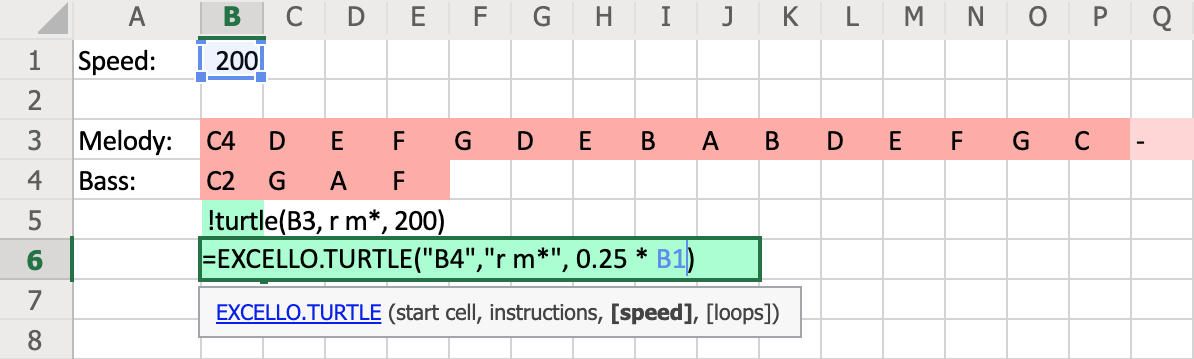
\includegraphics[width=150mm]{figs/turtleFunction.png}}
\caption{Defining a turtle using the \texttt{EXCELLO.TURTLE} function.}
\label{implementation:turtleFunction}
\end{figure}

\vspace{-30pt}
\texttt{\subsubsection{EXCELLO.MODULATE}}

\paragraph{} A modulating function lets melodic lines be defined by the intervals between notes and provides easy modulation of existing sections of a piece. The function takes a cell and an interval and outputs the cell with any notes transposed by the interval, maintaining any dynamics. A section can be modulated by calling this function on the first note with a provided interval and then using drag-fill. By using the previous note and one of a series of intervals as the arguments, a melodic line can quickly be produced from a starting note and a series of intervals as shown in Figure \ref{implementation:modulateFunction}.

\begin{figure}[tbh]
\centerline{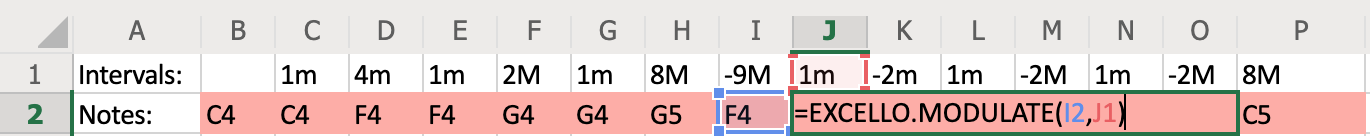
\includegraphics[width=150mm]{figs/modulateFunction.png}}
\caption{Transposing notes using the \texttt{EXCELLO.MODULATE} function.}
\label{implementation:modulateFunction}
\end{figure}

%  \ref{examples}

\subsection{Sustain}

\paragraph{} To prevent confusion between the south instruction and sustains. The symbol ``\texttt{-}" sustains a note. This was chosen because it is light and also has some similarity to a tie.\footnote{A line used in musical notation to increase the length of a note by joining it to another note.} Again, to maintain backwards compatibility, ``\texttt{s}" in a cell is still interpreted as a sustain.

\subsection{Active Turtles}

\paragraph{} To show that active turtle definitions have been recognised, a list of locations of the active turtles is given below the play button. This also helps find spurious turtles not intended to be activated.

\subsection{Automatic Movement}

\paragraph{} To prevent counting the cells in a line, \texttt{m*} instructs a turtle to move as far as there are notes or sustains defined in the direction it is facing. After adding more notes, the turtle instructions do not need editing before pressing play. A part may be meant to finish with a number of rests. As rests are notated with blank cells, a method to extend the path to include these rests was required. A cell can be explicitly defined as a rest with ``\texttt{.}". This is required if multiple turtles are playing a repeating section where one turtle's final cell as a note, sustain or multi-note cell. Without an explicit rest, the turtle would repeat too soon and the parts would consequently be out of phase.

\subsection{Inferred Octave}

\paragraph{} Octave numbers are inferred if omitted. Two methods were considered. Firstly, as most intervals within melodic lines are small, the nearest note could be played.
% This means that a scale would only need the octave defining in the first note.
Whilst this may require the fewest explicit statements of octave numbers, it would be hard to immediately identify the octave of any given note. The last defined octave in the path would need finding and then all subsequent notes walked through keeping track of the octave. The second consideration was to always use the last defined octave. Whilst this may require many octave definitions around the boundary between octaves, it is easier to find the octave of a note by backtracking. The second option was therefore implemented.

\subsection{Chords}

\paragraph{} To aid entering common chords, common types are repeated in a section at the top of the type drop-down. The chord drop-downs layout has been improved with labels to make it clearer what the values refer to. If the notes were entered vertically, the order was reversed, increasing correspondence with traditional staff notation.

\subsection{Activation of turtles}

\paragraph{} A ``Toggle Activation" button was added to the add-in window. When a cell or range is highlighted in the spreadsheet, the activation of any turtle definitions in this range will be toggled when the button is pressed.  This significantly decreases the time to toggle activations, as only two clicks are required, rather than entering the cell edit mode to add or remove an exclamation mark.

\section{Final Prototype Implementation}

\paragraph{} This section discusses the underlying implementation of the final prototype, following the participatory design. Excello consists of three main parts: the turtle system for playing the grid contents, the chord input tool, and the custom Excel functions.

\paragraph{} When the play button is pressed, turtle definitions in the grid are identified. For each, the starting cell and movement instructions are used to establish the contents of the cells it passes through. This is converted to a series of note definitions - pitch, start time, duration, volume. The speed and loop parameters are used to create the structure interpreted by the Tone.js library to schedule and initiate playback. An overview of the data flow and subtasks required to create the musical playback is shown in Figure \ref{fig:overview}.

\begin{figure}[htb]
\begin{center}
  
  \tikzset{every picture/.style={line width=0.75pt}} %set default line width to 0.75pt

  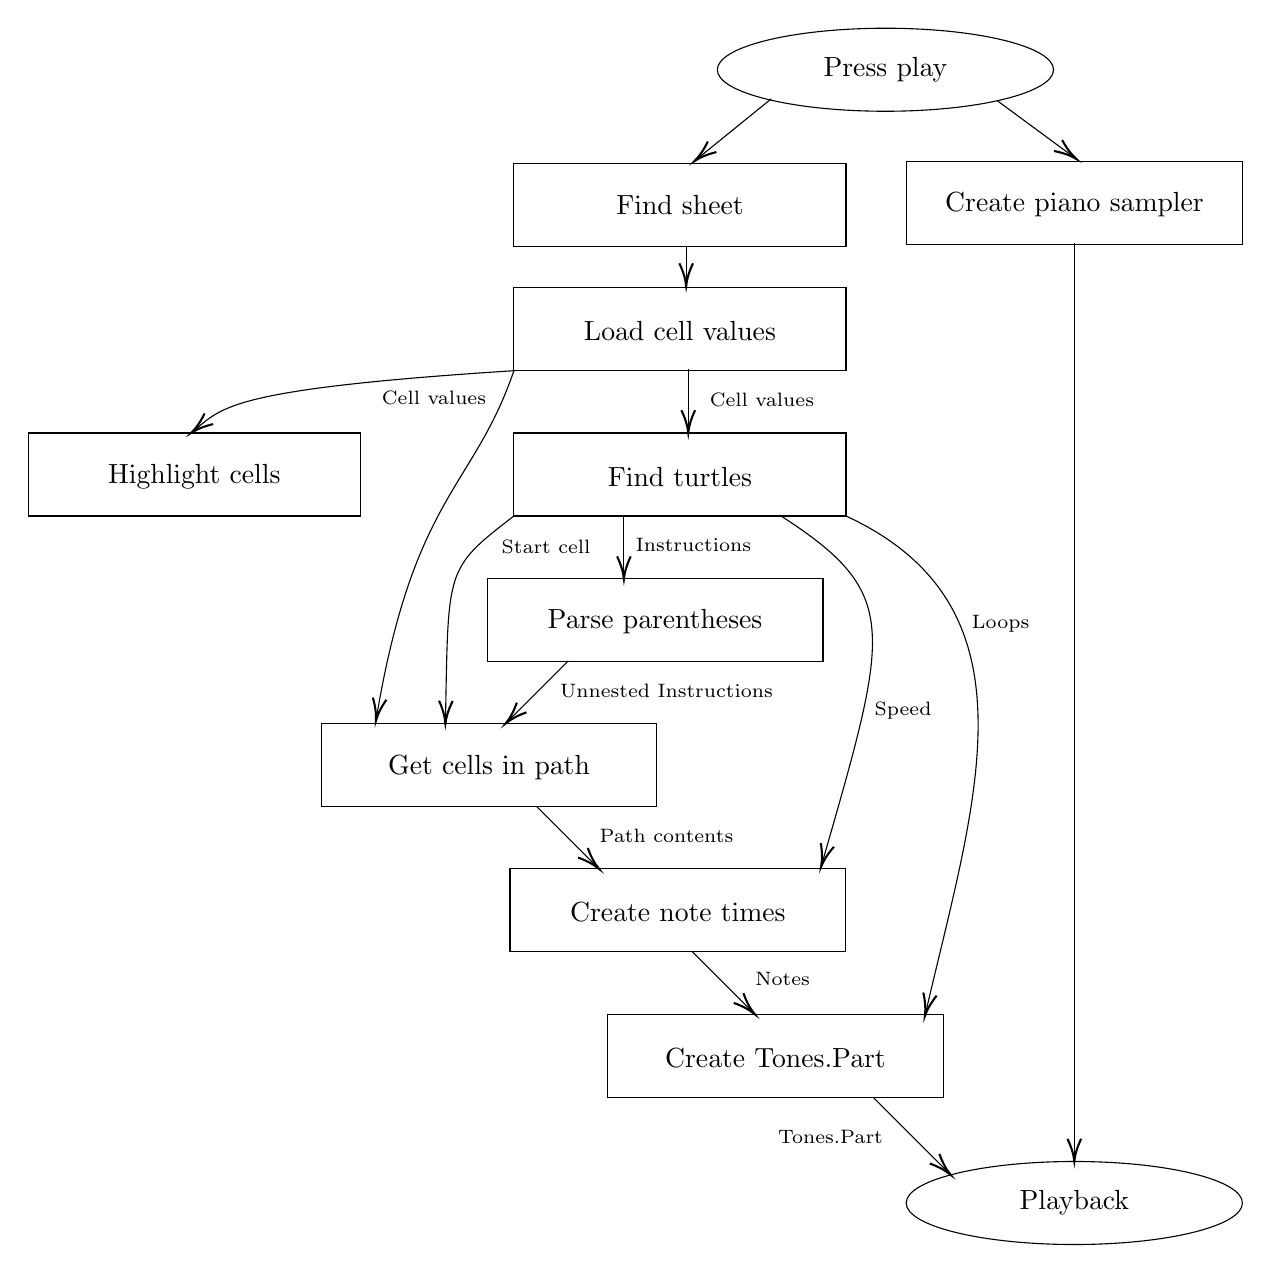
\begin{tikzpicture}[x=0.75pt,y=0.75pt,yscale=-1,xscale=1]
  %uncomment if require: \path (0,604); %set diagram left start at 0, and has height of 604

  %Shape: Rectangle [id:dp3390223975782729]
  \draw   (244.5,71) -- (404.5,71) -- (404.5,111) -- (244.5,111) -- cycle ;

  %Shape: Rectangle [id:dp7168559924493858]
  \draw   (244.5,131) -- (404.5,131) -- (404.5,171) -- (244.5,171) -- cycle ;

  %Shape: Rectangle [id:dp8835932361497658]
  \draw   (433.7,70) -- (595.5,70) -- (595.5,110) -- (433.7,110) -- cycle ;

  %Shape: Rectangle [id:dp9464422191216635]
  \draw   (244.5,201) -- (404.5,201) -- (404.5,241) -- (244.5,241) -- cycle ;

  %Shape: Rectangle [id:dp6384624480751633]
  \draw   (231.6,271) -- (393.4,271) -- (393.4,311) -- (231.6,311) -- cycle ;

  %Shape: Rectangle [id:dp2927464084046889]
  \draw   (151.6,341) -- (313.4,341) -- (313.4,381) -- (151.6,381) -- cycle ;

  %Shape: Rectangle [id:dp9052659554068596]
  \draw   (242.6,411) -- (404.4,411) -- (404.4,451) -- (242.6,451) -- cycle ;

  %Shape: Rectangle [id:dp5637329489183025]
  \draw   (289.6,481) -- (451.4,481) -- (451.4,521) -- (289.6,521) -- cycle ;

  %Curve Lines [id:da3917180624639185]
  \draw    (244.5,241) .. controls (211.17,266.67) and (212.98,265.81) .. (211.52,339.88) ;
  \draw [shift={(211.5,341)}, rotate = 271.14] [color={rgb, 255:red, 0; green, 0; blue, 0 }  ][line width=0.75]    (10.93,-3.29) .. controls (6.95,-1.4) and (3.31,-0.3) .. (0,0) .. controls (3.31,0.3) and (6.95,1.4) .. (10.93,3.29)   ;

  %Straight Lines [id:da6961662223442007]
  \draw    (297.5,241) -- (297.5,269.4) ;
  \draw [shift={(297.5,271.4)}, rotate = 270] [color={rgb, 255:red, 0; green, 0; blue, 0 }  ][line width=0.75]    (10.93,-3.29) .. controls (6.95,-1.4) and (3.31,-0.3) .. (0,0) .. controls (3.31,0.3) and (6.95,1.4) .. (10.93,3.29)   ;

  %Curve Lines [id:da9168950950169605]
  \draw    (372.6,240.6) .. controls (431.31,278.41) and (425.56,294.84) .. (392.99,408.28) ;
  \draw [shift={(392.5,410)}, rotate = 286.01] [color={rgb, 255:red, 0; green, 0; blue, 0 }  ][line width=0.75]    (10.93,-3.29) .. controls (6.95,-1.4) and (3.31,-0.3) .. (0,0) .. controls (3.31,0.3) and (6.95,1.4) .. (10.93,3.29)   ;

  %Curve Lines [id:da7972588626438504]
  \draw    (404.5,241) .. controls (499.03,284.78) and (466.83,377.07) .. (442.86,480.44) ;
  \draw [shift={(442.5,482)}, rotate = 282.99] [color={rgb, 255:red, 0; green, 0; blue, 0 }  ][line width=0.75]    (10.93,-3.29) .. controls (6.95,-1.4) and (3.31,-0.3) .. (0,0) .. controls (3.31,0.3) and (6.95,1.4) .. (10.93,3.29)   ;

  %Straight Lines [id:da6822022155717844]
  \draw    (270.7,310.8) -- (241.91,339.59) ;
  \draw [shift={(240.5,341)}, rotate = 315] [color={rgb, 255:red, 0; green, 0; blue, 0 }  ][line width=0.75]    (10.93,-3.29) .. controls (6.95,-1.4) and (3.31,-0.3) .. (0,0) .. controls (3.31,0.3) and (6.95,1.4) .. (10.93,3.29)   ;

  %Straight Lines [id:da4884596231580207]
  \draw    (255.5,381) -- (284.09,409.59) ;
  \draw [shift={(285.5,411)}, rotate = 225] [color={rgb, 255:red, 0; green, 0; blue, 0 }  ][line width=0.75]    (10.93,-3.29) .. controls (6.95,-1.4) and (3.31,-0.3) .. (0,0) .. controls (3.31,0.3) and (6.95,1.4) .. (10.93,3.29)   ;

  %Straight Lines [id:da9233366942734922]
  \draw    (330.5,451) -- (359.09,479.59) ;
  \draw [shift={(360.5,481)}, rotate = 225] [color={rgb, 255:red, 0; green, 0; blue, 0 }  ][line width=0.75]    (10.93,-3.29) .. controls (6.95,-1.4) and (3.31,-0.3) .. (0,0) .. controls (3.31,0.3) and (6.95,1.4) .. (10.93,3.29)   ;

  %Straight Lines [id:da3670498457872964]
  \draw    (417.5,521) -- (453.49,556.99) ;
  \draw [shift={(454.9,558.4)}, rotate = 225] [color={rgb, 255:red, 0; green, 0; blue, 0 }  ][line width=0.75]    (10.93,-3.29) .. controls (6.95,-1.4) and (3.31,-0.3) .. (0,0) .. controls (3.31,0.3) and (6.95,1.4) .. (10.93,3.29)   ;

  %Straight Lines [id:da28794703530347365]
  \draw    (327.5,111) -- (327.5,128.2) ;
  \draw [shift={(327.5,130.2)}, rotate = 270] [color={rgb, 255:red, 0; green, 0; blue, 0 }  ][line width=0.75]    (10.93,-3.29) .. controls (6.95,-1.4) and (3.31,-0.3) .. (0,0) .. controls (3.31,0.3) and (6.95,1.4) .. (10.93,3.29)   ;

  %Straight Lines [id:da33376731250782754]
  \draw    (328.5,170) -- (328.5,199) ;
  \draw [shift={(328.5,201)}, rotate = 270] [color={rgb, 255:red, 0; green, 0; blue, 0 }  ][line width=0.75]    (10.93,-3.29) .. controls (6.95,-1.4) and (3.31,-0.3) .. (0,0) .. controls (3.31,0.3) and (6.95,1.4) .. (10.93,3.29)   ;

  %Curve Lines [id:da2676626927985757]
  \draw    (244.5,171) .. controls (225.1,227.72) and (196.29,230.77) .. (178.27,338.17) ;
  \draw [shift={(178,339.8)}, rotate = 279.38] [color={rgb, 255:red, 0; green, 0; blue, 0 }  ][line width=0.75]    (10.93,-3.29) .. controls (6.95,-1.4) and (3.31,-0.3) .. (0,0) .. controls (3.31,0.3) and (6.95,1.4) .. (10.93,3.29)   ;

  %Straight Lines [id:da024649031996502035]
  \draw    (514.5,109.6) -- (514.5,550) ;
  \draw [shift={(514.5,552)}, rotate = 270] [color={rgb, 255:red, 0; green, 0; blue, 0 }  ][line width=0.75]    (10.93,-3.29) .. controls (6.95,-1.4) and (3.31,-0.3) .. (0,0) .. controls (3.31,0.3) and (6.95,1.4) .. (10.93,3.29)   ;

  %Shape: Ellipse [id:dp13505581605963868]
  \draw   (433.5,572) .. controls (433.5,560.95) and (469.76,552) .. (514.5,552) .. controls (559.24,552) and (595.5,560.95) .. (595.5,572) .. controls (595.5,583.05) and (559.24,592) .. (514.5,592) .. controls (469.76,592) and (433.5,583.05) .. (433.5,572) -- cycle ;

  %Shape: Ellipse [id:dp006287630832967794]
  \draw   (342.5,26) .. controls (342.5,14.95) and (378.76,6) .. (423.5,6) .. controls (468.24,6) and (504.5,14.95) .. (504.5,26) .. controls (504.5,37.05) and (468.24,46) .. (423.5,46) .. controls (378.76,46) and (342.5,37.05) .. (342.5,26) -- cycle ;

  %Straight Lines [id:da09048722077694915]
  \draw    (368.5,40) -- (333.05,68.74) ;
  \draw [shift={(331.5,70)}, rotate = 320.96000000000004] [color={rgb, 255:red, 0; green, 0; blue, 0 }  ][line width=0.75]    (10.93,-3.29) .. controls (6.95,-1.4) and (3.31,-0.3) .. (0,0) .. controls (3.31,0.3) and (6.95,1.4) .. (10.93,3.29)   ;

  %Straight Lines [id:da9578993167654264]
  \draw    (477.5,41) -- (513.89,67.81) ;
  \draw [shift={(515.5,69)}, rotate = 216.38] [color={rgb, 255:red, 0; green, 0; blue, 0 }  ][line width=0.75]    (10.93,-3.29) .. controls (6.95,-1.4) and (3.31,-0.3) .. (0,0) .. controls (3.31,0.3) and (6.95,1.4) .. (10.93,3.29)   ;

  %Shape: Rectangle [id:dp25073410390478523]
  \draw   (10.5,201) -- (170.5,201) -- (170.5,241) -- (10.5,241) -- cycle ;

  %Curve Lines [id:da2454539812308738]
  \draw    (244.5,171) .. controls (108.92,179.69) and (104.17,188.37) .. (90.53,199.75) ;
  \draw [shift={(89,201)}, rotate = 321.34000000000003] [color={rgb, 255:red, 0; green, 0; blue, 0 }  ][line width=0.75]    (10.93,-3.29) .. controls (6.95,-1.4) and (3.31,-0.3) .. (0,0) .. controls (3.31,0.3) and (6.95,1.4) .. (10.93,3.29)   ;


  % Text Node
  \draw (324.5,91) node  [align=left] {Find sheet};
  % Text Node
  \draw (324.5,152) node  [align=left] {Load cell values};
  % Text Node
  \draw (514.6,91) node  [align=left] {Create piano sampler};
  % Text Node
  \draw (324.5,222) node  [align=left] {Find turtles};
  % Text Node
  \draw (312.5,292) node  [align=left] {Parse parentheses};
  % Text Node
  \draw (232.5,362) node  [align=left] {Get cells in path};
  % Text Node
  \draw (323.5,432) node  [align=left] {Create note times};
  % Text Node
  \draw (370.5,502) node  [align=left] {Create Tones.Part};
  % Text Node
  \draw (514.5,572) node [] [align=left] {\textcolor[rgb]{0,0,0}{Playback}};
  % Text Node
  \draw (260,256) node  [align=left] {{\scriptsize Start cell}};
  % Text Node
  \draw (331,255) node  [align=left] {{\scriptsize Instructions}};
  % Text Node
  \draw (432,335) node  [align=left] {{\scriptsize Speed}};
  % Text Node
  \draw (479,293) node  [align=left] {{\scriptsize Loops}};
  % Text Node
  \draw (318,325) node  [align=left] {{\scriptsize Unnested Instructions}};
  % Text Node
  \draw (318,395) node  [align=left] {{\scriptsize Path contents}};
  % Text Node
  \draw (374,464) node  [align=left] {{\scriptsize Notes}};
  % Text Node
  \draw (397,540) node  [align=left] {{\scriptsize Tones.Part}};
  % Text Node
  \draw (206,184) node  [align=left] {{\scriptsize Cell values}};
  % Text Node
  \draw (423.5,26) node [] [align=left] {Press play};
  % Text Node
  \draw (364,185) node  [align=left] {{\scriptsize Cell values}};
  % Text Node
  \draw (90.5,222) node  [align=left] {Highlight cells};


  \end{tikzpicture}

\end{center}
\caption{An overview of the playback algorithm and dataflow of Excello\label{fig:overview}}
\end{figure}

\paragraph{} The \texttt{Sampler} is an extension of the \texttt{Tone.Instrument} class. This interpolates between pitched samples to create arbitrary notes. A sampler is loaded using the Salamander grand piano samples~\footnote{https://freepats.zenvoid.org/Piano/acoustic-grand-piano.html} which includes four pitches (out of a possible 12) per octave. This accurately interpolates notes whilst reducing loading times and storage requirements.

\subsection{Identifying Cells}

\paragraph{} A drop-down is populated with names loaded using the Office API. Having pressed play, the cell values from the selected sheet are loaded and then analysed for highlighting and calculating the musical output. Cells containing at least one note definition are highlighted red. A note must contain a note name, optional accidental, optional octave number, and optional volume instruction following a space. This is a dynamic marking or number between 0 and 1. Notes are identified using the following regular expression:

\begin{verbatim}
^[A-G](#|b|)?[1-9]?( (0(\.\[0-9]+)?|1(\.0)?|ppp|pp|p|mp|mf|f|ff|fff))?$
\end{verbatim}

\paragraph{} Cells containing multiple definitions (e.g. ``\texttt{C4 ff,-, ,D}", ``\texttt{,,G,F$\sharp$}") are split using commas. The resulting strings are trimmed of starting and ending whitespace and then must either be a note, sustain (``\texttt{-}" or ``\texttt{s}"), explicit rest (``\texttt{.}") or empty string (created from trimming a rest). Cells matching ``\texttt{-}",``\texttt{.}" or ``\texttt{s}" are highlighted a lighter red. Turtle definitions (e.g. ``\texttt{!turtle(B2:B4, r m*, 200, 1)}") are identified using:
\begin{verbatim}
^(!turtle\().*(\))$
\end{verbatim}
and these cells are highlighted green. The addresses of cells containing a turtle definition are added to the live turtle section of the add-in window.

\subsection{Parsing Movement Instructions}

\paragraph{} Movement instructions are converted to a single unnested list of commands (e.g.~``\texttt{(r m2)2}" becomes ``\texttt{[r, m2, r, m2]}") so the turtle's path can be established. The \texttt{parse} method of the Parenthesis\footnote{https://www.npmjs.com/package/parenthesis} library seemed suitable for aiding this string manipulation. This parses strings containing brackets into a nested array. For example, \texttt{parse(\textcolor[rgb]{0,0.7,0}{\upquote{a(b[c\{d\}])}})} gives \texttt{[\textcolor[rgb]{0,0.7,0}{\upquote{a(}}, [\textcolor[rgb]{0,0.7,0}{\upquote{b[}}, [\textcolor[rgb]{0,0.7,0}{\upquote{c\{}}, [\textcolor[rgb]{0,0.7,0}{\upquote{d}}], \textcolor[rgb]{0,0.7,0}{\upquote{\}}}], \textcolor[rgb]{0,0.7,0}{\upquote{]}}], \textcolor[rgb]{0,0.7,0}{\upquote{)}}]}.

\paragraph{} This suggests the string ``\texttt{(r m2)2}" would become \texttt{[\upquote{(}, [\upquote{r m2}], \upquote{)2}]}. By removing the brackets from these strings, a simple recursive method could be built to output \texttt{\upquote{r m2 r m2}} from \texttt{[[\upquote{r m2}], \upquote{2}]}. However, upon testing this, the library outputted an undefined array. From investigating the source code, I established that strings with a number following a closing parenthesis all produced this error. Substituting characters for the numbers or placing a symbol before all numbers and then later removing these would allow the library to be used. Instead, using the Parenthesis method as inspiration, I implemented my own parsing function tailored to Excello.

\paragraph{} This has two main steps. First, the deepest bracketed expression is stored in an array with the brackets removed. This expression is replaced in the original string with the string \upquote{\texttt{\_\_\_}$x$\texttt{\_\_\_}} where $x$ is the expression's index in the array. This is repeated until the string contains no brackets. Then a recursive function uses the values of $x$ to reconstruct the string in the nested array format. This method is outlined in Algorithm \ref{alg:parenthesis}. The Typescript implementation is in Appendix \ref{appendix:parseBrackets}.

\begin{algorithm}[!htp]
\caption{Parsing bracketed expression. \texttt{str.replace(regex,f)} (line 13) performs \texttt{f(s)} on the first substring, \texttt{s}, of \texttt{str} matching the regular expression \texttt{regex}.}
\label{alg:parenthesis}
\begin{algorithmic}[1]
\Procedure{parseBrackets}{$str$}

   \State $idPadding\gets \texttt{\upquote{\_\_\_}}$
   \State $unnestedStr\gets []$
   \State $deepestLevelBracketsRE\gets \texttt{RegExp(\upquote{\textbackslash\textbackslash([\^{}\textbackslash\textbackslash(\textbackslash\textbackslash)]*\textbackslash\textbackslash)})}$
   \State $replacementIDRE\gets \texttt{RegExp(\upquote{\textbackslash\textbackslash} + }idPadding\texttt{ + \upquote{([0-9]+)} + }idPadding\texttt{)}$\\

   \Procedure{replaceDeepestBracket}{$x$}
     \State \texttt{unnestedStr.push(x.substring(1, x.length-1))}
     \State \texttt{\textbf{return} idPadding + (unnestedStr.length - 1) + idPadding}
   \EndProcedure \\

   \While{\texttt{deepestLevelBracketsRE.test(str)}}
     \State \texttt{str = str.replace(deepestLevelBracketsRE,replaceDeepestBracket)}
   \EndWhile

   \State \texttt{unnestedStr[0] = str}\\

   \Procedure{reNest}{$outerStr$}
     \State $renestingStr\gets []$
     \While{There is a match of $replacementIDRE$ in $outerStr$}
       \State $matchIndex\gets$ index of the match in $outerStr$
       \State $matchID\gets$ ID of the match (number between padding)
       \State $matchString\gets$ matched string\\

       \If{$matchIndex >$ 0}
				\State $renestingStr$.push($outestStr$.substring(0, $matchIndex$))
			\EndIf
			\State $renestingStr$.push(reNest($unnestedStr$[$firstMatchID$]))
			\State $outestStr$ = $outestStr$.substring($matchIndex$ + $matchString$.length)
     \EndWhile
     \State $renestingStr$.push($outestStr$)
     \State \textbf{return} $renestingStr$
   \EndProcedure \\

   \State \textbf{return} \textsc{reNest}($unnestedStr$[0])

\EndProcedure
\end{algorithmic}
\end{algorithm}


\paragraph{} Having submitted a bug report on the Parenthesis GitHub, and implemented my own method for parsing turtle movement instructions, I implemented a fix to the Parenthesis library. The library previously performed replacements with the string \upquote{\texttt{\_\_\_}$x$}. $x$ and following numbers would concatenate forming a single number, causing the library to fail. My method of having an identifier before and after $x$ fixed this issue. I also added additional tests to Parenthesis to verify my method and ensure that previous tests all passed before submitting a pull request. I have made an open source contribution, as this has since been merged into the library and published.

\paragraph{} I wrote an additional recursive method to unnest the array into a single stream of commands. An empty string, \texttt{s}, is initialised. For each item in the array, if it is an array, unnest the contents recursively and add the result to s. If not, it will be one or more single movement commands. If the single movement commands start with a number, the result is added to \texttt{s} that number of times. The remaining instructions are added to \texttt{s}. This is outlined in Algorithm \ref{alg:unnest}. The implementation is shown in Appendix \ref{appendix:processParsedBrackets}.

\begin{algorithm}[!htbp]
\caption{Unnesting parsed bracketed expressions.}
\label{alg:unnest}
\begin{algorithmic}[1]
\Procedure{processParsedBrackets}{$arr$}

   \State $s\gets \texttt{\upquote{}}$
   \State $previousArr$

   \For{$v$ in $s$}
    \If{$v$ is an array}
     \State $previousArr \gets$ processParsedBrackets($v$)
    \Else
       \If{previous instruction was an array}
        \State $s \gets s + previousArr$
        \If{next instruction is a number}
          \State $s \gets s + previousArr$, that number of times minus one
        \EndIf
       \EndIf
       \State $s \gets s + $ remaining instruction in $v$
    \EndIf
   \EndFor
   \State \textbf{return} $s$

\EndProcedure
\end{algorithmic}
\end{algorithm}

\subsection{Getting Cells in Turtles' Paths}

\paragraph{} If the turtle's first argument defines a range of starting cells, the cell addresses of this range are calculated. For each starting cell, the unnested instructions and sheet values are used to find the contents of the cells the turtle passes through. This process models the movement of the turtle within the grid, keeping track of its position and the direction in which it is facing. For each instruction, the position and direction are updated as required, and the contents of any new cells entered are added to a list of notes.

\paragraph{} For the ``\texttt{m*}" instruction, the number of steps the turtle takes must be computed. Given the turtle's current position and direction, the one-dimensional array of cells in front of it is taken. The turtle should step to the last cell that defines a note, sustain or explicit rest. The number of steps is the array's length minus the index of the first element in the reversed array satisfying this criterion.

\subsection{Creating Note Times}

\paragraph{} The cells a turtle moves through are used to create a data structure containing the information for playback using the Tone library. For each turtle, the following array is produced: \texttt{[[<Note 1>,...,<Note N>], <number of cells>]} (note sequence array). Each note is as follows: \texttt{[<start time>, [<pitch>, <duration>, <volume>]]}. Volume and octave are added to each note if they were omitted from a cell.

\paragraph{} The Tone Transport is a timeline along which events can be scheduled. This supports many different representations of time. I used Transport Time for all note onsets and durations. This is of the form \texttt{\upquote{BARS:QUARTERS:SIXTEENTHS}} where the three values are numbers and can be non-integer. With \texttt{QUARTERS} representing the number of cells, the calculation of exact times, or arbitrary musical notes can be avoided. This allows the contents of cells to be easily converted to times to be interpreted by the Tones library.

\paragraph{} The note sequence array is initiated by counting the notes that are defined in the cell contents using regular expressions for identifying notes and multi-note cells. The cells are iterated through keeping track of the active note and adding it to the note sequence when it ends. Outside of this loop, variables track how many cells and notes through the process the algorithm is and whether it is currently a rest or note. Variables keep track of the note currently being played - when it started (\texttt{currentStart}), the pitch (\texttt{currentNote}) and the volume (\texttt{currentVolume}). As volume and octave number may be omitted, variables also keep track of these. Table \ref{tab:times} outlines the actions performed when a cell is read. Notes are added to the note sequence in the form \texttt{[currentStart, [currentNote, \upquote{0:} + noteLength + \upquote{:0}, currentVolume]]}.

\begin{table}[ht]
\begin{tabular}{|l|l|l|l|l|}
  \hline
  \textbf{Cell}&\textbf{State}&\multicolumn{3}{c|}{\textbf{Action}} \\
  \hline
  \multirow{5}{*}{Note}&\multirow{3}{*}{Note}&Note, octave and &Previous note added&currentStart = \\
  &&volume established&to note sequence&\upquote{0:}+beatCount+\upquote{:0}\\
  &&from cell contents&&currentNote = value\\
  \cline{2-2}
  \cline{4-4}
  &\multirow{2}{*}{Rest}&and previous values&inRest = false&noteLength = 1\\
  &&&&currentVolume = volume\\
  \hline
  \multirow{2}{*}{Sustain}&Note&\multicolumn{3}{l|}{noteLength++}\\
  \cline{2-5}
  &Rest&\multicolumn{3}{l|}{Nothing (has no semantic value)}\\
  \hline
  \multirow{3}{*}{Rest}&\multirow{2}{*}{Note}&\multicolumn{3}{l|}{Previous note added to note sequence}\\
  &&\multicolumn{3}{l|}{inRest = true}\\
  \cline{2-5}
  &Rest&\multicolumn{3}{l|}{Nothing}\\
  \hline
\end{tabular}
\caption{The actions taken when processing each cell to create note times. The beat count corresponds to the cell number being processed and is incremented each time.\label{tab:times}}
\end{table}
\vspace{-10pt}

\paragraph{} The same method is used for multi-note cells, except the note length and cell count are incremented by the appropriate fraction for each item in the cell. If, after the final cell, the state is a note, it is ended and added to the note sequence.

\paragraph{} The values in the note sequence are sufficient for the piano sampler to play a note using the \texttt{triggerAttackRelease} function. The \texttt{Tone.Part} class allows multiple calls to this method to be defined, started, stopped and looped as a single unit. This is defined with the note sequence and its speed set with the evaluated turtle speed argument. The number of cells, calculated when creating the note times, number of repeats, and the evaluated speed argument are used to control when looping ends.

% \begin{verbatim}
% var turtlePart = new Tone.Part(function(time, note){
%   piano.triggerAttackRelease(note[0], note[1], time, note[2]);
% }, noteTimes).start();
% if (repeats>0){
%   turtlePart = turtlePart.stop("0:" + (repeats*beatsLength/speedFactor) + ":0");
% }
% turtlePart.loop = true;
% turtlePart.loopEnd = "0:" + beatsLength + ":0";
% turtlePart.playbackRate = speedFactor;
% \end{verbatim}

% \begin{lstlisting}[style=js]
%   var turtlePart = new Tone.Part(function(time, note){
%     piano.triggerAttackRelease(note[0], note[1], time, note[2]);
%   }, noteTimes).start();
%   if (repeats>0){
%     turtlePart = turtlePart.stop("0:" + (repeats*beatsLength/speedFactor) + ":0");
%   }
%   turtlePart.loop = true;
%   turtlePart.loopEnd = "0:" + beatsLength + ":0";
%   turtlePart.playbackRate = speedFactor;
% \end{lstlisting}

\subsection{Chord Input}\label{Chord Input}

\paragraph{} The next two subsections (\S\ref{Chord Input} and \S\ref{Custom Excel Functions}) outline the two smaller parts of the Excello; the chord input tool, and the custom Excel functions. When the insert button in the add-in window is pressed, the note, type, inversion and octave of the chord are extracted from their HTML elements. The chord interface within the add-in window is shown in Figure \ref{fig:chordInput}. The tonal library is used to generate the chord notes:

\begin{verbatim}
var chordNotes = Chord.notes(chordNote, chordType).map(x => Note.simplify(x));
\end{verbatim}
\vspace{-10pt}

\begin{figure}[htb]
\centerline{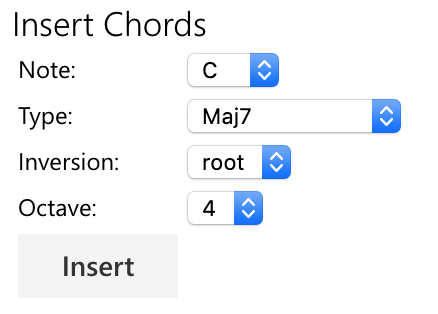
\includegraphics[width=50mm]{figs/insertChord.png}}
\caption{The interface within the add-in window for inserting the notes of chords.}
\label{fig:chordInput}
\end{figure}

\vspace{-20pt}
\paragraph{} The tonal \texttt{simplify} function reduces note definitions to contain at most one accidental, as required by Excello. This provides a list of notes in ascending order, without octaves or taking into account the inversion. To create the correct inversion of the chord, the array of notes is rotated by the inversion number.

\paragraph{} The given octave number is appended to the first note. A dictionary matches note names, accounting for enharmonics,\footnote{Notes that are the same pitch but different names, such as A$\flat$ and G$\sharp$.} to position in the chromatic scale starting at C (the first note of the octave in SPN). For each preceding note, if it appears in an equal or lower position in the scale than its predecessor, the octave number is incremented before appending. Otherwise, it is in the same octave, so the octave number is appended without modification.

\paragraph{} The selected range is acquired with the Office API. The chord notes are entered starting at the top-left corner of this range. If the range's height is greater or equal to its width, the notes are entered vertically going down. Otherwise, they are entered horizontally going right. Using the Office API, the range is set to the 2D array where the chord is entered.

\subsection{Custom Excel Functions}\label{Custom Excel Functions}

\paragraph{} Custom functions are implemented using another add-in. Rather than a separate window like the main Excello add-in, additional functions can be used in cells with the prefix ``\texttt{=EXCELLO.}". The file structure was generated with the Yeoman generator. The name, description, result type, and parameter names and types are stored in a JSON schema. This is used by Excel to provide argument prompts and autofill when writing formulae. Functions are defined in Typescript.

\paragraph{} The turtle function concatenates the arguments into the Excello turtle format. Other cells can be referenced, for example, the speed variable can reference a global tempo variable as in Figure \ref{implementation:turtleFunction}.

\paragraph{} The modulation function separates the note and volume for every note defined in a cell. The note is modulated using the tonal \texttt{Distance.transpose} function and recombined with the volume. The drag fill feature of Excel can be employed by the user to transpose sections or define melodic lines using the interval between notes as in Figure \ref{implementation:modulateFunction}.

\section{MIDI Converter}

\paragraph{} This section explains the Python converter from MIDI to CSV for Excello playback. A MIDI file is divided into up to 16 parallel tracks~\cite{midiSpec}. Each track contains a series of messages defined using predefined status and data bytes. I used the Mido library\footnote{https://mido.readthedocs.io/en/latest/index.html} to read MIDI files and abstract away from the underlying byte representations to view the messages. Note onsets and offsets are two separate events with two separate messages~\cite{midiSpec}. These messages include the note pitch, velocity, channel (not relevant) and time in ticks since the last message~\cite{midoSpec}.

\paragraph{} First, the list of messages is converted to a list of notes defined by onset and offset time, pitch and velocity. For each track, the messages are iterated through, using the time value in every message (including control and meta messages) to update a variable tracking time. For note onset messages, this is added to a dictionary mapping pitch to a list of currently active note start times. Lists are used because a pitch can be active multiple times at once. For note offset messages, or onset messages with zero velocity, the note popped from the active notes at that pitch with end time added is added to the list of all notes defined in the file.

\paragraph{} As each turtle only plays one note at a time, the notes are split into lists so no list contains concurrently played notes. Provided the initial list of notes is non-empty, a new list is created. The first remaining note is moved to the new list. Then iterating over the remaining notes, the next note starting after the previous note ends is moved to this new list. The number of iterations required is the number of turtles, $n$.

\paragraph{} If every tick corresponds to a cell, any combination of note onsets and offsets in a MIDI file can be accurately represented in Excello. To achieve smaller representations, the start and end times are converted to smaller cell numbers within the path of the turtle. For many MIDI files, the duration of a note is different from the time it occupies in notation. For example, a note immediately followed by another note in notation may have an end time significantly less than the start time of the next note in MIDI. A method is required to account for this. For all notes, before creating the different turtle streams, the length of the notes in ticks and differences between consecutive start times are found. The minimum value greater than 1 or modal value for these times are calculated depending on the compression level giving the $lengthStat$ and $di\hspace{-0.1em}f\hspace{-0.2em}f\hspace{-0.1em}erenceStat$.
\vspace{-10pt}

  $$ratio_{int} = \lfloor\max(lengthStat, di\hspace{-0.1em}f\hspace{-0.2em}f\hspace{-0.1em}erenceStat)/\min(lengthStat, di\hspace{-0.1em}f\hspace{-0.2em}f\hspace{-0.1em}erenceStat)\rfloor$$
  % $$ratio_{int} = \lfloor ratio \rfloor$$
  % $$correction = ratio/ratio_{int}$$
For each note, the times are adjusted as follows:
  $$length \gets (start - end) / lengthStat \text{ (rounded to the nearest 0.1)}$$
  $$start \gets start / di\hspace{-0.1em}f\hspace{-0.2em}f\hspace{-0.1em}erenceStat \times ratio_{int} \text{ (rounded to the nearest 0.1)}$$
  $$end \gets start +length$$

\paragraph{} The streams, with note start and end times corresponding to cells, are converted to a CSV file for Excello. Each turtle's path is initialised as an array of empty strings with length equal to the maximum end time for a note in any turtle, $L$. Each note the turtle plays is entered into the array. MIDI defines pitch using the integers. As there are 12 notes in an octave, modulus and division with 12 gives the note name and octave for SPN. If velocity is different from the previous note played by the turtle (or the note is the first note), the eight-bit MIDI velocity is mapped to Excello's [0,1] range. If the note length is greater than one, sustains are placed in the following cells. These paths go right starting in column A, with the first in row 2.

\paragraph{} Finally, the turtle definition is placed in the spreadsheet. The start cell range is ``A2:A$(n+1)$". The movement instruction is ``r m$L$". The MIDI file contains meta data for the \texttt{tempo} (milliseconds per beat) and \texttt{ticks\_per\_beat}. Cells per minute is calculated as follows:
$$cells\ per\ tick \times ticks\ per\ beat \times beat\ per\ minute$$
$$= \frac{ratio_{int}}{di\hspace{-0.1em}f\hspace{-0.2em}f\hspace{-0.1em}erenceStat} \times \texttt{ticks\_per\_beat} \times \frac{60 \times 10^6}{\texttt{tempo}}$$
With a value of 1 for repeats, the turtle definition is put in cell A1 and the CSV exported.

\newpage
\section{Repository Overview}

\tikzstyle{dir}=[draw=black,thick,anchor=west]
\tikzstyle{src}=[draw=black,thick,anchor=west,fill=red!30]
\tikzstyle{file}=[draw=black,thick,anchor=west,draw=none]

\begin{wrapfigure}{r}{8cm}
\vspace{-15pt}
% \begin{figure}[tbh]
\begin{tikzpicture}[%
  grow via three points={one child at (0.5,-0.7) and
  two children at (0.5,-0.7) and (0.5,-1.4)},
  edge from parent path={(\tikzparentnode.south) |- (\tikzchildnode.west)}]
  \node [dir] {Excello}
    child { node [dir] {Excel Music}
      child { node [dir] {assets}}
      child { node [dir] {node\_modules}}
      child { node [dir] {src}
        child { node [file] {index.ts}}
        child { node [file] {turtle.ts}}
        child { node [file] {chords.ts}}
        child { node [file] {regex.ts}}
        child { node [file] {conversions.ts}}
        child { node [file] {bracketsParse.ts}}
      }
      child [missing] {}
      child [missing] {}
      child [missing] {}
      child [missing] {}
      child [missing] {}
      child [missing] {}
      child { node [file] {index.html}}
      child { node [file] {manifest.xml}}
    }
    child [missing] {}
    child [missing] {}
    child [missing] {}
    child [missing] {}
    child [missing] {}
    child [missing] {}
    child [missing] {}
    child [missing] {}
    child [missing] {}
    child [missing] {}
    child [missing] {}
    child { node [dir] {CustomFunctions}
      child { node [dir] {src}
        child { node [file] {excello.ts}}
      }
      child [missing] {}
      child { node [dir] {config}
        child { node [file] {excello.json}}
      }
      child [missing] {}
      child { node [dir] {node\_modules}}
      child { node [file] {manifest.xml}}
    }
    child [missing] {}
    child [missing] {}
    child [missing] {}
    child [missing] {}
    child [missing] {}
    child [missing] {}
    child { node [dir] {MIDI}
      child { node [file] {MIDI\_Conversion.ipynb}}
    };
\end{tikzpicture}
\caption{File structure overview showing original files}
\label{fig:repo}
\vspace{-30pt}
% \end{figure}
\end{wrapfigure}

\paragraph{} Figure \ref{fig:repo} shows a reduced project file structure including all original source code. Excel Music is the add-in that parses the notation and produces music. Both this and CustomFunctions were generated using the Yeomann generator. The manifest.xml files are added to Excel and point to the resources to run the add-in. Users were given a different manifest pointing to a distribution hosted online with Surge. node\_modules contains all libraries required to run the add-ins and is managed using npm.

\paragraph{} The index.html file defines the window that appears on the right of the spreadsheet. assets contains the piano samples. index.ts defines what happens when the buttons of the window are pressed and imports from the remaining Typescript files. turtle.ts contains all the code to produce musical output from the spreadsheet, with helper functions in regex.ts, conversions.ts and bracketsParse.ts. bracketsParse.ts was based on Parenthesis which was initially incompatible for Excello's needs. chords.ts is for inserting chord notes into the grid.

\paragraph{} customFunctions.ts contains the implementation of EXCELLO.TURTLE and EXCELLO.MODULATE. The index.html file created when generating this add-in is not seen by the user so was not re-written.

\paragraph{} The Python notebook MIDI\_Conversion.ipynb converts MIDI files to the Excello notation. Conversions of MIDI corpora are included in the MIDI directory.

\paragraph{} I shall release Excello as an open source project under the MIT license. This is compatible with the MIT licenses of the libraries. The Salamander piano samples come under a creative commons license\footnote{https://creativecommons.org/licenses/by/3.0/.} so credit shall be given in the Excel add-in window.



% TC:ignore

%%%%%%%%%%%%%%%%%%%%%%%%%%%%%%%%%%%%%%%%%%%%%%%%%%%%%%%%%%%%%%%%%%%%%
% the bibliography
\addcontentsline{toc}{chapter}{Bibliography}
\bibliography{refs}

%%%%%%%%%%%%%%%%%%%%%%%%%%%%%%%%%%%%%%%%%%%%%%%%%%%%%%%%%%%%%%%%%%%%%
% the appendices
\appendix

\chapter{Brackets Parsing Implementation}

\section{parseBrackets}
\label{appendix:parseBrackets}
\begin{lstlisting}[style=js]
// inspiration taken from:
// https://github.com/dy/parenthesis/blob/master/index.js

/**
 * Given a turtle instruction sequence this unwraps any brackets to create exact instrutions
 * @param str Turtle movement instructions e.g. "(r m3)4"
 * @return explicit unwrapped instructions e.g. "r m3 r m3 r m3 r m3"
 */
export function parseBrackets(str: string) {

	var unnestedStr = ['will become highest level'];
	var idPadding = '__';

	var deepestLevelBracketsRE = new RegExp('\\([^\\(\\)]*\\)'); // finds bracket with no brackets inside

	// store contents of bracket it unnestedStr and replace contents in str with ID
	while (deepestLevelBracketsRE.test(str)) {
		str = str.replace(deepestLevelBracketsRE,function(x) {
			unnestedStr.push(x.substring(1, x.length-1)); // add the token without the brackets
			return idPadding + (unnestedStr.length - 1) + idPadding;
		});
	}
	unnestedStr[0] = str; // make first element in array the highest level of the string

	var replacementIDRE = new RegExp('\\' + idPadding + '([0-9]+)' + idPadding);

	// transform references to tree
	function reNest (outestStr: string) {
		var renestingStr = [];
		var match;

		while (match = replacementIDRE.exec(outestStr)) {

			var matchIndex = match.index;
			var firstMatchID = match[1];
			var fullStringMatched = match[0];

			// push what was before
			if (matchIndex > 0) {
				renestingStr.push(outestStr.substring(0, matchIndex))
			}
			//perform recursively
			renestingStr.push(reNest(unnestedStr[firstMatchID]))
			// remove the string that has been processed
			outestStr = outestStr.substring(matchIndex + fullStringMatched.length)
		}
		renestingStr.push(outestStr)
		return renestingStr
	}

	return reNest(unnestedStr[0])
}
\end{lstlisting}

\section{processParsedBrackets}
\label{appendix:processParsedBrackets}
\begin{lstlisting}[style=js]
export function processParsedBrackets(arr) {
	var s = "";
	var wasPrevArray = false;
	var prevArray = "";
	for (let val of arr) {
		if (val.constructor === Array) {
			prevArray = processParsedBrackets(val)
			wasPrevArray = true;
		}
		else {
			var singleInstructions = val.trim().split(" ");
			if (wasPrevArray) {
				s = s + prevArray;
				if (!isNaN(singleInstructions[0])) {
					for (var i=1; i<singleInstructions[0]; i++) {
						s = s + prevArray;
					}
					singleInstructions = singleInstructions.slice(1);
				}
			}
			for (let instruction of singleInstructions) {
				s = s + instruction + " ";
			}
			wasPrevArray = false;
		}
	}
	if (wasPrevArray) {
		s = s + prevArray;
	}
	return s;
}
\end{lstlisting}

% \chapter{Project Proposal}

\includepdf[pages=-]{chapters/proposalAnon}

% TC:endignore

\end{document}
